% Options for packages loaded elsewhere
% Options for packages loaded elsewhere
\PassOptionsToPackage{unicode}{hyperref}
\PassOptionsToPackage{hyphens}{url}
\PassOptionsToPackage{dvipsnames,svgnames,x11names}{xcolor}
%
\documentclass[
  11pt,
  letterpaper,
  DIV=11,
  numbers=noendperiod]{scrreprt}
\usepackage{xcolor}
\usepackage[top=0.75in,bottom=0.75in,left=0.75in,right=0.75in]{geometry}
\usepackage{amsmath,amssymb}
\setcounter{secnumdepth}{-\maxdimen} % remove section numbering
\usepackage{iftex}
\ifPDFTeX
  \usepackage[T1]{fontenc}
  \usepackage[utf8]{inputenc}
  \usepackage{textcomp} % provide euro and other symbols
\else % if luatex or xetex
  \usepackage{unicode-math} % this also loads fontspec
  \defaultfontfeatures{Scale=MatchLowercase}
  \defaultfontfeatures[\rmfamily]{Ligatures=TeX,Scale=1}
\fi
\usepackage{lmodern}
\ifPDFTeX\else
  % xetex/luatex font selection
\fi
% Use upquote if available, for straight quotes in verbatim environments
\IfFileExists{upquote.sty}{\usepackage{upquote}}{}
\IfFileExists{microtype.sty}{% use microtype if available
  \usepackage[]{microtype}
  \UseMicrotypeSet[protrusion]{basicmath} % disable protrusion for tt fonts
}{}
\makeatletter
\@ifundefined{KOMAClassName}{% if non-KOMA class
  \IfFileExists{parskip.sty}{%
    \usepackage{parskip}
  }{% else
    \setlength{\parindent}{0pt}
    \setlength{\parskip}{6pt plus 2pt minus 1pt}}
}{% if KOMA class
  \KOMAoptions{parskip=half}}
\makeatother
% Make \paragraph and \subparagraph free-standing
\makeatletter
\ifx\paragraph\undefined\else
  \let\oldparagraph\paragraph
  \renewcommand{\paragraph}{
    \@ifstar
      \xxxParagraphStar
      \xxxParagraphNoStar
  }
  \newcommand{\xxxParagraphStar}[1]{\oldparagraph*{#1}\mbox{}}
  \newcommand{\xxxParagraphNoStar}[1]{\oldparagraph{#1}\mbox{}}
\fi
\ifx\subparagraph\undefined\else
  \let\oldsubparagraph\subparagraph
  \renewcommand{\subparagraph}{
    \@ifstar
      \xxxSubParagraphStar
      \xxxSubParagraphNoStar
  }
  \newcommand{\xxxSubParagraphStar}[1]{\oldsubparagraph*{#1}\mbox{}}
  \newcommand{\xxxSubParagraphNoStar}[1]{\oldsubparagraph{#1}\mbox{}}
\fi
\makeatother


\usepackage{longtable,booktabs,array}
\usepackage{calc} % for calculating minipage widths
% Correct order of tables after \paragraph or \subparagraph
\usepackage{etoolbox}
\makeatletter
\patchcmd\longtable{\par}{\if@noskipsec\mbox{}\fi\par}{}{}
\makeatother
% Allow footnotes in longtable head/foot
\IfFileExists{footnotehyper.sty}{\usepackage{footnotehyper}}{\usepackage{footnote}}
\makesavenoteenv{longtable}
\usepackage{graphicx}
\makeatletter
\newsavebox\pandoc@box
\newcommand*\pandocbounded[1]{% scales image to fit in text height/width
  \sbox\pandoc@box{#1}%
  \Gscale@div\@tempa{\textheight}{\dimexpr\ht\pandoc@box+\dp\pandoc@box\relax}%
  \Gscale@div\@tempb{\linewidth}{\wd\pandoc@box}%
  \ifdim\@tempb\p@<\@tempa\p@\let\@tempa\@tempb\fi% select the smaller of both
  \ifdim\@tempa\p@<\p@\scalebox{\@tempa}{\usebox\pandoc@box}%
  \else\usebox{\pandoc@box}%
  \fi%
}
% Set default figure placement to htbp
\def\fps@figure{htbp}
\makeatother

\ifLuaTeX
  \usepackage{luacolor}
  \usepackage[soul]{lua-ul}
\else
  \usepackage{soul}
\fi




\setlength{\emergencystretch}{3em} % prevent overfull lines

\providecommand{\tightlist}{%
  \setlength{\itemsep}{0pt}\setlength{\parskip}{0pt}}



 


\usepackage{float}
\usepackage{booktabs}
\KOMAoption{captions}{tableheading}
\makeatletter
\@ifpackageloaded{tcolorbox}{}{\usepackage[skins,breakable]{tcolorbox}}
\@ifpackageloaded{fontawesome5}{}{\usepackage{fontawesome5}}
\definecolor{quarto-callout-color}{HTML}{909090}
\definecolor{quarto-callout-note-color}{HTML}{0758E5}
\definecolor{quarto-callout-important-color}{HTML}{CC1914}
\definecolor{quarto-callout-warning-color}{HTML}{EB9113}
\definecolor{quarto-callout-tip-color}{HTML}{00A047}
\definecolor{quarto-callout-caution-color}{HTML}{FC5300}
\definecolor{quarto-callout-color-frame}{HTML}{acacac}
\definecolor{quarto-callout-note-color-frame}{HTML}{4582ec}
\definecolor{quarto-callout-important-color-frame}{HTML}{d9534f}
\definecolor{quarto-callout-warning-color-frame}{HTML}{f0ad4e}
\definecolor{quarto-callout-tip-color-frame}{HTML}{02b875}
\definecolor{quarto-callout-caution-color-frame}{HTML}{fd7e14}
\makeatother
\makeatletter
\@ifpackageloaded{bookmark}{}{\usepackage{bookmark}}
\makeatother
\makeatletter
\@ifpackageloaded{caption}{}{\usepackage{caption}}
\AtBeginDocument{%
\ifdefined\contentsname
  \renewcommand*\contentsname{Table of contents}
\else
  \newcommand\contentsname{Table of contents}
\fi
\ifdefined\listfigurename
  \renewcommand*\listfigurename{List of Figures}
\else
  \newcommand\listfigurename{List of Figures}
\fi
\ifdefined\listtablename
  \renewcommand*\listtablename{List of Tables}
\else
  \newcommand\listtablename{List of Tables}
\fi
\ifdefined\figurename
  \renewcommand*\figurename{Figure}
\else
  \newcommand\figurename{Figure}
\fi
\ifdefined\tablename
  \renewcommand*\tablename{Table}
\else
  \newcommand\tablename{Table}
\fi
}
\@ifpackageloaded{float}{}{\usepackage{float}}
\floatstyle{ruled}
\@ifundefined{c@chapter}{\newfloat{codelisting}{h}{lop}}{\newfloat{codelisting}{h}{lop}[chapter]}
\floatname{codelisting}{Listing}
\newcommand*\listoflistings{\listof{codelisting}{List of Listings}}
\makeatother
\makeatletter
\makeatother
\makeatletter
\@ifpackageloaded{caption}{}{\usepackage{caption}}
\@ifpackageloaded{subcaption}{}{\usepackage{subcaption}}
\makeatother
\usepackage{bookmark}
\IfFileExists{xurl.sty}{\usepackage{xurl}}{} % add URL line breaks if available
\urlstyle{same}
\hypersetup{
  pdftitle={Vic Cicconetti --- This Is Your Life},
  pdfauthor={The Cicconetti Family},
  colorlinks=true,
  linkcolor={blue},
  filecolor={Maroon},
  citecolor={Blue},
  urlcolor={Blue},
  pdfcreator={LaTeX via pandoc}}


\title{Vic Cicconetti --- This Is Your Life}
\usepackage{etoolbox}
\makeatletter
\providecommand{\subtitle}[1]{% add subtitle to \maketitle
  \apptocmd{\@title}{\par {\large #1 \par}}{}{}
}
\makeatother
\subtitle{A Tribute on His 80th Birthday}
\author{The Cicconetti Family}
\date{2026-03-01}
\begin{document}
\maketitle

\renewcommand*\contentsname{Table of contents}
{
\hypersetup{linkcolor=}
\setcounter{tocdepth}{1}
\tableofcontents
}

\bookmarksetup{startatroot}

\chapter*{Dedication}\label{dedication}
\addcontentsline{toc}{chapter}{Dedication}

\markboth{Dedication}{Dedication}

\emph{For Dad --- veteran, educator, entrepreneur, family man.}

\emph{From Bayonne to Vietnam, from the classroom to the family table,
yours has been a life of service, love, and laughter. This book is our
way of saying what you sign every email:}

{Love, Your Family}

\begin{center}\rule{0.5\linewidth}{0.5pt}\end{center}

\textbf{March 2026} --- Eighty years. A life that stretches from the
streets of Bayonne to the skies over Vietnam, from the hallways of New
Jersey's public schools to the warmth of a family dinner table. This is
the story of Victor R. Cicconetti --- veteran, educator, entrepreneur,
community leader, husband, father, and grandfather. A man whose life
truly is, as one newspaper described it, ``an American story.''

\part{Part I: Two Families}

\chapter{Two Families, One City}\label{roots}

\emph{In the early 1900s, two families left southern Italy --- one from
the mountains of Abruzzo, one from the hills of Campania. They crossed
the Atlantic, passed through Ellis Island, and landed in the same small
city on the New Jersey waterfront. They didn't know each other yet. But
their grandchildren would marry, and this story would begin.}

\begin{tcolorbox}[enhanced jigsaw, left=2mm, leftrule=.75mm, opacityback=0, breakable, colframe=quarto-callout-note-color-frame, toprule=.15mm, bottomrule=.15mm, colback=white, arc=.35mm, rightrule=.15mm]
\begin{minipage}[t]{5.5mm}
\textcolor{quarto-callout-note-color}{\faInfo}
\end{minipage}%
\begin{minipage}[t]{\textwidth - 5.5mm}

\vspace{-3mm}\textbf{Soundtrack: Bayonne Doo-Wop \& The Crooners (1950s--early '60s)}\vspace{3mm}

Vic grew up in Bayonne in the 1950s --- fifteen minutes from Newark, the
doo-wop capital of the world. This is what was coming out of every
transistor radio, corner candy store, and church dance in his
neighborhood:

\textbf{Doo-Wop (the sound of Bayonne)} --- \emph{click any song to
play}

\begin{itemize}
\tightlist
\item
  \href{https://www.youtube.com/watch?v=Bs037jwD3_A}{Dion \& The
  Belmonts --- ``A Teenager in Love''} /
  \href{https://www.youtube.com/watch?v=ik57HLn0Nm0}{Dion ---
  ``Runaround Sue''}
\item
  \href{https://www.youtube.com/watch?v=jMcWldfg28s}{The Four Seasons
  --- ``Sherry''} /
  \href{https://www.youtube.com/watch?v=zRZpaxBMJRU}{The Four Seasons
  --- ``Big Girls Don't Cry''} \emph{(Frankie Valli = Jersey royalty)}
\item
  \href{https://www.youtube.com/watch?v=PSddD6w5SKc}{The Drifters ---
  ``Under the Boardwalk''} \emph{(the Jersey Shore anthem)}
\item
  \href{https://www.youtube.com/watch?v=FvzNeh4Mq1o}{The Flamingos ---
  ``I Only Have Eyes for You''}
\item
  \href{https://www.youtube.com/watch?v=RBj2HN2uuNA}{The Platters ---
  ``The Great Pretender''} /
  \href{https://www.youtube.com/watch?v=vfBboBz3yoc}{The Platters ---
  ``Smoke Gets in Your Eyes''}
\item
  \href{https://www.youtube.com/watch?v=2sAHiR0rkJg}{Frankie Lymon \&
  The Teenagers --- ``Why Do Fools Fall in Love''}
\item
  \href{https://www.youtube.com/watch?v=lPV5FrydqDE}{Danny \& The
  Juniors --- ``At the Hop''}
\item
  \href{https://www.youtube.com/watch?v=hEolAR08m9s}{The Del-Vikings ---
  ``Come Go with Me''}
\end{itemize}

\textbf{The Italian-American Crooners (what the parents played)}

\begin{itemize}
\tightlist
\item
  \href{https://www.youtube.com/watch?v=RUz1pZ_LujU}{Dean Martin ---
  ``That's Amore''} /
  \href{https://www.youtube.com/watch?v=ah637P0_cts}{Dean Martin ---
  ``Volare''}
\item
  \href{https://www.youtube.com/watch?v=Y2rDb4Ur2dw}{Frank Sinatra ---
  ``Fly Me to the Moon''} /
  \href{https://www.youtube.com/watch?v=C1AHec7sfZ8}{Frank Sinatra ---
  ``I've Got You Under My Skin''}
\item
  \href{https://www.youtube.com/watch?v=ZZ_hWTuSYSk}{Perry Como ---
  ``Magic Moments''} /
  \href{https://www.youtube.com/watch?v=_VJlHWESyLI}{Perry Como ---
  ``Catch a Falling Star''}
\item
  \href{https://www.youtube.com/watch?v=5Ws60MDF7OY}{Connie Francis ---
  ``Who's Sorry Now''} \emph{(she's from Newark!)}
\item
  \href{https://www.youtube.com/watch?v=QSGVD2DgWy8}{Louis Prima ---
  ``Just a Gigolo''} /
  \href{https://www.youtube.com/watch?v=5CXZB-dIF0g}{Louis Prima ---
  ``Buona Sera''}
\item
  \href{https://www.youtube.com/watch?v=m8OlDPqYBLw}{Bobby Darin ---
  ``Beyond the Sea''} /
  \href{https://www.youtube.com/watch?v=557lFG-qq5g}{Bobby Darin ---
  ``Mack the Knife''}
\end{itemize}

\emph{What did Grandma Eleanor play in the kitchen? What songs does Dad
hum when he smells Sunday sauce?
\href{https://docs.google.com/forms/d/e/1FAIpQLSdpYXns7Zwutq6tDNp3BYU2HCPTHTgkdok6r9xWPpdXVPbvCQ/viewform}{Suggest
a song →} --- we'll add the best suggestions to the final playlist.}

\end{minipage}%
\end{tcolorbox}

\begin{tcolorbox}[enhanced jigsaw, toptitle=1mm, opacitybacktitle=0.6, leftrule=.75mm, breakable, toprule=.15mm, colbacktitle=quarto-callout-note-color!10!white, titlerule=0mm, left=2mm, opacityback=0, colframe=quarto-callout-note-color-frame, bottomtitle=1mm, title=\textcolor{quarto-callout-note-color}{\faInfo}\hspace{0.5em}{The World Vic Was Born Into (1946)}, arc=.35mm, colback=white, coltitle=black, rightrule=.15mm, bottomrule=.15mm]

\textbf{Consider what a Bayonne household looked like the year Victor
Cicconetti was born:}

The family had a \textbf{rotary telephone} --- one, on the wall, shared
by the whole house. Long distance cost real money, so you kept it short.
The \textbf{radio} was the center of entertainment: Jack Benny, The
Shadow, the evening news. If the family had a \textbf{television} at
all, it arrived around 1948--50 --- a small screen, black and white,
three channels if you were lucky, and you adjusted the rabbit ears by
hand. The \textbf{icebox} was transitioning to an electric refrigerator.
Clothes went through a \textbf{wringer washer} --- no dryer, they hung
on the line. Dad drove a car with a manual choke, no seatbelts, no power
steering. Mom cooked on a gas stove and preserved food by canning.

There was no air conditioning. No microwave. No answering machine. No
calculator --- you did math by hand or with a slide rule. A ``computer''
was a room-sized machine at a university. The ballpoint pen had just
been invented. Frozen dinners didn't exist yet. Neither did the
interstate highway system, the polio vaccine, or rock and roll.

\textbf{This is the world Victor was born into.} By the time he turns
80, he will have lived through:

\begin{itemize}
\tightlist
\item
  \textbf{Rotary phone → smartphone} (1946 → now)
\item
  \textbf{Three TV channels → 500 channels → streaming} (1950 → 1990 →
  2015)
\item
  \textbf{Slide rule → pocket calculator → laptop → AI} (1946 → 1972 →
  1990 → 2023)
\item
  \textbf{Vinyl records → 8-track → cassette → CD → MP3 → Spotify}
  (every format, in order)
\item
  \textbf{Handwritten letters → email → text → FaceTime} (the entire arc
  of communication)
\item
  \textbf{No commercial flights → moon landing → Space Shuttle → Mars
  rovers} (1946 → 1969 → 1981 → 2021)
\end{itemize}

No generation in human history witnessed more technological change in a
single lifetime than the one born in the mid-1940s. Vic didn't just
watch it happen --- he embraced it. He was the teacher who wrote grants
for Commodore computers when other educators thought it was a fad. He
was the dad who had a VIC-20 in the house in 1982. He was the man who,
at 79, forwards emails from his desktop and uses his phone to stay in
touch with grandchildren spread across the country.

The distance from a Bayonne icebox to a smartphone in your pocket ---
that's one lifetime. That's \emph{his} lifetime.

\end{tcolorbox}

\section{The Great Departure}\label{the-great-departure}

\begin{tcolorbox}[enhanced jigsaw, toptitle=1mm, opacitybacktitle=0.6, leftrule=.75mm, breakable, toprule=.15mm, colbacktitle=quarto-callout-note-color!10!white, titlerule=0mm, left=2mm, opacityback=0, colframe=quarto-callout-note-color-frame, bottomtitle=1mm, title=\textcolor{quarto-callout-note-color}{\faInfo}\hspace{0.5em}{The Bigger Picture: Why 4 Million Italians Left}, arc=.35mm, colback=white, coltitle=black, rightrule=.15mm, bottomrule=.15mm]

\textbf{The broadest wavelet:} Between 1880 and 1924, over \textbf{four
million Italians} emigrated to the United States --- the largest
single-nationality migration in American history. They were
overwhelmingly from the \emph{Mezzogiorno} (the south): Campania,
Calabria, Sicily, Abruzzo, Puglia. Italy had unified in 1861, but
unification made things worse for the south. Northern industrialists
taxed southern agriculture to fund northern factories. Inheritance laws
divided farms into smaller and smaller plots until a family couldn't
feed itself on what it owned.

\textbf{Push factors:} Poverty. Malaria. Cholera. Earthquakes (Messina,
1908: 75,000 dead). A feudal land system that hadn't changed in
centuries. The \emph{contadini} (peasant farmers) had no path forward.

\textbf{Pull factors:} American industry needed labor. Steel mills, coal
mines, railroads, oil refineries, garment factories --- all of it
demanded bodies willing to work for wages that, while pitiful by
American standards, dwarfed anything available in a stone village in the
Apennines. Letters home from relatives already in America --- the
\emph{lettere di richiamo} --- described a world where work was hard but
food was plentiful and a man could own a house.

\textbf{The numbers:} In peak years (1900--1914), over 200,000 southern
Italians arrived annually at Ellis Island. The flow was so enormous that
entire villages depopulated. Collepietro --- the Cicconetti homeland ---
has fewer than 200 residents today.

\end{tcolorbox}

\begin{tcolorbox}[enhanced jigsaw, toptitle=1mm, opacitybacktitle=0.6, leftrule=.75mm, breakable, toprule=.15mm, colbacktitle=quarto-callout-note-color!10!white, titlerule=0mm, left=2mm, opacityback=0, colframe=quarto-callout-note-color-frame, bottomtitle=1mm, title=\textcolor{quarto-callout-note-color}{\faInfo}\hspace{0.5em}{The Journey: Steerage Class to Ellis Island}, arc=.35mm, colback=white, coltitle=black, rightrule=.15mm, bottomrule=.15mm]

\textbf{The mid wavelet --- what the crossing actually looked like:}

The journey began with a walk. From mountain villages like Collepietro,
families traveled by mule or on foot to the nearest rail station, then
by train to \textbf{Naples} --- the great embarkation port for southern
Italians. There, emigration agents processed their paperwork and sold
them passage.

\textbf{The ship:} Steerage class. The cheapest tickets (roughly \$30
--- about \$1,000 today). Passengers were packed below the waterline in
open compartments with tiered metal bunks, no ventilation, and one
toilet per hundred people. The crossing took \textbf{12 to 17 days}.
Seasickness was universal. Many had never seen the ocean before
boarding.

\textbf{Ellis Island:} The Statue of Liberty appeared first --- most
immigrants saw her from the deck of the ship, crowded against the
railing. Then the ferry to Ellis Island. Then the \textbf{Great Hall}: a
vast, echoing room where thousands waited in metal-railed lines,
clutching their documents.

The inspection had three stages:

\begin{enumerate}
\def\labelenumi{\arabic{enumi}.}
\item
  \textbf{Medical exam} --- Doctors watched immigrants climb the stairs
  to the Great Hall, looking for limps, labored breathing, signs of
  disease. The dreaded \textbf{``buttonhook men''} used a small hook to
  flip back eyelids, checking for trachoma (an eye disease that meant
  automatic deportation). A chalk mark on your coat --- \textbf{X} for
  mental deficiency, \textbf{H} for heart, \textbf{L} for limp --- sent
  you to a detention room.
\item
  \textbf{Legal inspection} --- An officer asked 29 questions: name,
  age, occupation, final destination, how much money you carried (you
  needed at least \$25), whether anyone was meeting you, whether you'd
  ever been in prison. Interpreters translated. The whole interview
  lasted about two minutes.
\item
  \textbf{The Staircase of Separation} --- Three aisles. Left: New York.
  Center: detained for further review. Right: New Jersey ferry. Families
  who'd survived the crossing together could be separated here in an
  instant.
\end{enumerate}

\textbf{The success rate:} About \textbf{98\%} of immigrants who reached
Ellis Island were admitted. But that 2\% rejection rate --- roughly
250,000 people between 1892 and 1924 --- meant that every person in that
line knew it could happen to them. Ellis Island's Italian nickname was
\emph{L'Isola delle Lacrime} --- \textbf{the Island of Tears}.

\end{tcolorbox}

\begin{tcolorbox}[enhanced jigsaw, toptitle=1mm, opacitybacktitle=0.6, leftrule=.75mm, breakable, toprule=.15mm, colbacktitle=quarto-callout-note-color!10!white, titlerule=0mm, left=2mm, opacityback=0, colframe=quarto-callout-note-color-frame, bottomtitle=1mm, title=\textcolor{quarto-callout-note-color}{\faInfo}\hspace{0.5em}{US Immigration Policy: The Door Opens, Then Closes}, arc=.35mm, colback=white, coltitle=black, rightrule=.15mm, bottomrule=.15mm]

\textbf{The policy wavelet:}

\begin{itemize}
\tightlist
\item
  \textbf{1882:} First federal immigration law. Barred ``lunatics,
  idiots, and persons likely to become a public charge.''
\item
  \textbf{1892:} Ellis Island opens as the federal immigration station.
  Before this, states ran their own processing (Castle Garden in
  Manhattan handled New York).
\item
  \textbf{1907:} Peak year --- \textbf{1.25 million immigrants}
  processed through Ellis Island. Over 100 nationalities. The building
  was designed for 500,000.
\item
  \textbf{1917:} Literacy test required. Immigrants had to read 30--40
  words in their native language. This hit southern Italians hard ---
  many were illiterate.
\item
  \textbf{1921:} Emergency Quota Act. First numerical limit on
  immigration. Capped each nationality at 3\% of its 1910 Census
  population in the US.
\item
  \textbf{1924:} Johnson-Reed Act. \textbf{Slashed quotas to 2\% of the
  1890 Census} --- deliberately targeting southern and eastern
  Europeans. Italian immigration dropped from 200,000/year to under
  4,000. The door slammed shut.
\end{itemize}

The Cicconettis and the Chiarolanzas made it through before the door
closed. Had they waited a decade, this story would never have happened.

\end{tcolorbox}

\section{From Italy to Bayonne}\label{from-italy-to-bayonne}

\subsection{The Cicconettis}\label{the-cicconettis}

\textbf{Origin:} Collepietro, Province of L'Aquila, Abruzzo --- a stone
village perched at 2,785 feet in the Apennine Mountains, fewer than 200
inhabitants even today.

\textbf{The name:} Cicconetti derives from \emph{Franciscus} (``a free
man'') through Italian diminutives: Francesco → Cicco → Cicconetti ---
``little Cicco.'' Documented in Collepietro since at least
\textbf{1778}, when \textbf{Camillo Giovanni Cicconetti} married Maria
Consiglia Iannarelli.

\textbf{The pronunciation --- and the war over it:} In Italian,
Cicconetti is pronounced with a hard \emph{ch}:
\textbf{``Chee-ko-NET-tee.''} That's how the old country said it. That's
how part of the family still says it. But Vic was adamant: the name gets
the \textbf{Americanized soft C} --- \textbf{``Sih-ko-NET-tee.''}

It wasn't vanity. It was survival. Growing up in Bayonne, a kid with a
name that started with ``Chick-'' was a sitting duck. \emph{``Hey,
Chicken Head, get over here!''} --- the playground taunts that
Italian-American kids absorbed like body blows. Every strange surname
was ammunition. Every rolled R was a target. The children of immigrants
learned fast: you either Americanize or you fight every single day.

Vic chose to Americanize. The soft C was a declaration: \emph{I am from
here. This is my country. Say my name the way I tell you to say it.} It
was the same instinct that drove the whole immigrant project --- don't
just arrive, \emph{belong}. Don't just survive, \emph{assimilate}. And
if the old-country pronunciation has to bend to make that happen, then
it bends.

To this day, the family is split. Some Cicconettis use the Italian
pronunciation. Some use Vic's Americanized version. It's a tiny civil
war that plays out every time someone new asks, ``How do you say your
last name?'' --- and the answer depends on which branch you're talking
to.

\textbf{Why they left:} Between 1880 and 1920, half a million Abruzzesi
left Italy. The soil was thin, the winters harsh, inheritance laws
fragmented the land. Young men traveled down from the mountains to
Naples, boarded steamships, crossed the Atlantic in steerage, and passed
through Ellis Island.

\textbf{Where they landed:} Bayonne, New Jersey --- a city of oil
refineries and shipyards on a narrow peninsula jutting into New York
Harbor. By 1920, Italians constituted over 20\% of the population. The
Cicconettis settled among other Abruzzese \emph{paesani}, near
\textbf{Assumption Catholic Church}.

\subsection{The Elias \& Chiarolanzas}\label{the-elias-chiarolanzas}

\textbf{Origin:} The Elia surname traces to southern Italy --- most
concentrated in \textbf{Puglia}, with presence in Calabria, Campania,
and Sicily. Yvonne's mother Mary carried the surname
\textbf{Chiarolanza} (Americanized to ``Chirolanza'') --- a rare name
meaning \textbf{``Bright Lance''} (\emph{chiara} + \emph{lanza}), rooted
in \textbf{Montecorvino Rovella, Province of Salerno, Campania}.

\textbf{The crossing:} The 1940 Census found \textbf{Mary Chiarolanza,
age 20}, in Bayonne with her father \textbf{Alfonso}, mother
\textbf{Angelina}, and \textbf{four sisters}. They had emigrated from
Campania and passed through Ellis Island.

\textbf{Where they landed:} The same city. Bayonne. The Elia family
settled near \textbf{Our Lady of Mount Carmel Church} (established 1899)
--- the heart of the Italian community, just blocks from the
Cicconettis. Mary Chiarolanza went to work as a \textbf{seamstress at
the Maidenform factory} at 154 Avenue E --- Bayonne's largest employer,
where Italian-American women sewed garments (and during WWII, parachutes
and carrier pigeon vests).

\textbf{Frank Elia} --- who worked as a poultry processor in Bayonne's
live markets --- married Mary Chiarolanza.

\begin{tcolorbox}[enhanced jigsaw, toptitle=1mm, opacitybacktitle=0.6, leftrule=.75mm, breakable, toprule=.15mm, colbacktitle=quarto-callout-note-color!10!white, titlerule=0mm, left=2mm, opacityback=0, colframe=quarto-callout-note-color-frame, bottomtitle=1mm, title=\textcolor{quarto-callout-note-color}{\faInfo}\hspace{0.5em}{Check Our Work --- The Old Country}, arc=.35mm, colback=white, coltitle=black, rightrule=.15mm, bottomrule=.15mm]

\begin{longtable}[]{@{}
  >{\raggedright\arraybackslash}p{(\linewidth - 8\tabcolsep) * \real{0.0732}}
  >{\raggedright\arraybackslash}p{(\linewidth - 8\tabcolsep) * \real{0.2683}}
  >{\centering\arraybackslash}p{(\linewidth - 8\tabcolsep) * \real{0.1463}}
  >{\centering\arraybackslash}p{(\linewidth - 8\tabcolsep) * \real{0.1707}}
  >{\centering\arraybackslash}p{(\linewidth - 8\tabcolsep) * \real{0.3415}}@{}}
\toprule\noalign{}
\begin{minipage}[b]{\linewidth}\raggedright
\#
\end{minipage} & \begin{minipage}[b]{\linewidth}\raggedright
We wrote\ldots{}
\end{minipage} & \begin{minipage}[b]{\linewidth}\centering
TRUE
\end{minipage} & \begin{minipage}[b]{\linewidth}\centering
FALSE
\end{minipage} & \begin{minipage}[b]{\linewidth}\centering
I DON'T KNOW
\end{minipage} \\
\midrule\noalign{}
\endhead
\bottomrule\noalign{}
\endlastfoot
1 & The Cicconetti name traces to Collepietro, Abruzzo & & & \\
2 & The Chiarolanza family came from Campania, likely Montecorvino
Rovella & & & \\
3 & Mary Chiarolanza worked at the Maidenform factory & & & \\
4 & Frank Elia worked as a poultry processor & & & \\
\end{longtable}

\textbf{Anything wrong? Fill in what we missed:}

\hfill\break

\end{tcolorbox}

\begin{tcolorbox}[enhanced jigsaw, toptitle=1mm, opacitybacktitle=0.6, leftrule=.75mm, breakable, toprule=.15mm, colbacktitle=quarto-callout-tip-color!10!white, titlerule=0mm, left=2mm, opacityback=0, colframe=quarto-callout-tip-color-frame, bottomtitle=1mm, title=\textcolor{quarto-callout-tip-color}{\faLightbulb}\hspace{0.5em}{Tell Us a Story}, arc=.35mm, colback=white, coltitle=black, rightrule=.15mm, bottomrule=.15mm]

\textbf{Dad:} What kind of trouble did you get into growing up in
Bayonne? Did you and Dennis ever do something your parents \emph{still}
don't know about?

\textbf{Mom:} What's the dish your mother made that nobody since has
gotten right? Close your eyes --- what does the old kitchen smell like?

\end{tcolorbox}

\begin{tcolorbox}[enhanced jigsaw, toptitle=1mm, opacitybacktitle=0.6, leftrule=.75mm, breakable, toprule=.15mm, colbacktitle=quarto-callout-note-color!10!white, titlerule=0mm, left=2mm, opacityback=0, colframe=quarto-callout-note-color-frame, bottomtitle=1mm, title=\textcolor{quarto-callout-note-color}{\faInfo}\hspace{0.5em}{Map: Bayonne --- Where Two Families Lived}, arc=.35mm, colback=white, coltitle=black, rightrule=.15mm, bottomrule=.15mm]

The Cicconettis and the Elias lived within blocks of each other. This
map shows Victor's childhood addresses, both family churches, the
Maidenform factory, and Ellis Island --- where it all began.

\emph{Interactive map available in the online version.}

\end{tcolorbox}

\begin{tcolorbox}[enhanced jigsaw, toptitle=1mm, opacitybacktitle=0.6, leftrule=.75mm, breakable, toprule=.15mm, colbacktitle=quarto-callout-note-color!10!white, titlerule=0mm, left=2mm, opacityback=0, colframe=quarto-callout-note-color-frame, bottomtitle=1mm, title=\textcolor{quarto-callout-note-color}{\faInfo}\hspace{0.5em}{Bayonne: Why Here?}, arc=.35mm, colback=white, coltitle=black, rightrule=.15mm, bottomrule=.15mm]

\textbf{The local wavelet --- why two Italian families ended up on this
specific peninsula:}

Bayonne, New Jersey sits on a narrow spit of land between Newark Bay and
New York Harbor --- 1.2 square miles, surrounded by water on three
sides. In the early 1900s, it was an industrial powerhouse:
\textbf{Standard Oil} had its largest refinery here (the smell of
petroleum was the smell of the city), \textbf{Maidenform} sewed bras and
girdles (and during WWII, parachutes), and shipyards along the Kill Van
Kull built vessels for the Navy.

Industry meant jobs. Jobs meant immigrants. By 1920, Bayonne was over
\textbf{20\% Italian}, with clusters from specific regions: Abruzzesi
near Assumption Church, Campanians near Our Lady of Mount Carmel. This
wasn't random --- it was \textbf{chain migration}. One man from
Collepietro gets a job at the refinery, writes a letter home, and his
cousin follows. Then his cousin's cousin. Within a generation, an entire
village has relocated to a ten-block radius in New Jersey.

The Italian neighborhoods had their own economy: bakeries, butchers,
live poultry markets (where Frank Elia worked), vegetable gardens in
tiny backyards, wine made in basements. The old people spoke Italian;
the children spoke English at school and Italian at home. The church was
the center of everything --- feast days, weddings, funerals, Sunday
Mass, the social calendar of a community that had transplanted itself
4,000 miles but kept its roots.

\end{tcolorbox}

\begin{center}\rule{0.5\linewidth}{0.5pt}\end{center}

\section{The Unspoken Rule}\label{the-unspoken-rule}

Nobody sat you down and explained it. There was no speech, no family
meeting, no written contract. But every Italian-American kid who grew up
in a house like the Cicconettis' or the Elias' understood the deal ---
it was in the air, in the way your parents looked at you, in the silence
after a bad report card, in the pride that radiated off them when you
did something right:

\textbf{You better be advancing this family.}

That was the immigrant mentality, and it wasn't optional. Your
grandparents left everything --- their village, their language, their
parents' graves --- and crossed an ocean in steerage so that \emph{you}
could have more than they did. Your parents worked jobs that broke their
bodies --- refineries, factories, poultry markets, sewing machines ---
so that \emph{you} wouldn't have to. The debt was enormous, and it was
repaid in one currency: \textbf{progress}.

Every generation was expected to climb higher than the last:

\begin{itemize}
\tightlist
\item
  The \textbf{first generation} (the immigrants) did the crossing. They
  survived. They got jobs, learned enough English to function, and kept
  their families fed. That was the mission, and it was enough.
\item
  The \textbf{second generation} (Victor Sr., Frank Elia, Eleanor, Mary)
  was supposed to stabilize. Own a house. Stay out of trouble. Raise
  children who spoke English without an accent. Send them to school. Get
  them further from the boat.
\item
  The \textbf{third generation} (Vic, Yvonne) was supposed to
  \emph{arrive}. Get educated. Get a career --- not a job, a
  \emph{career}. Become professionals. Become Americans who nobody could
  look down on. And then raise children who went even further.
\end{itemize}

This wasn't pressure in the way modern parenting books describe
pressure. It was deeper than that. It was \emph{identity}. You didn't
advance just for yourself --- you advanced for every person who came
before you, for every sacrifice that made your life possible. When Vic
got his education degree, that wasn't just Vic succeeding. That was
Collepietro succeeding. That was the steerage crossing paying off. That
was the whole project of immigration being \emph{validated}.

And it worked. A poultry processor's daughter married a refinery
worker's grandson, and together they produced educators, technologists,
and professionals. The immigrant bet --- \emph{leave everything, cross
the ocean, work until your hands bleed, and trust that the children will
rise} --- that bet paid off, spectacularly, in the Cicconetti family.

But the mentality never fully left. Even now, even at eighty, Vic's
pride in his children's accomplishments --- ``Dearest Son, I hope you
can take a long breath and exhale!!!!'' --- carries the echo of a
grandfather he may never have met, standing on the deck of a steamship,
watching the Statue of Liberty appear through the fog, thinking:
\emph{this better be worth it}.

It was.

\begin{tcolorbox}[enhanced jigsaw, toptitle=1mm, opacitybacktitle=0.6, leftrule=.75mm, breakable, toprule=.15mm, colbacktitle=quarto-callout-note-color!10!white, titlerule=0mm, left=2mm, opacityback=0, colframe=quarto-callout-note-color-frame, bottomtitle=1mm, title=\textcolor{quarto-callout-note-color}{\faInfo}\hspace{0.5em}{The Italian-American Political Journey}, arc=.35mm, colback=white, coltitle=black, rightrule=.15mm, bottomrule=.15mm]

\textbf{The broadest wavelet:} The Italian-American political story is
one of the great migrations in American electoral history --- and it
mirrors the family's journey from survival to arrival.

\textbf{The FDR era (1930s--1960s):} The first and second generation
were \textbf{Democrats}, almost universally. FDR's New Deal fed them
during the Depression. Social Security, labor protections, public works
jobs --- these programs were lifelines for immigrant families hanging on
by their fingernails. The Democratic Party was the party of the working
man, and Italian-Americans were working men. In Bayonne, voting
Democratic was as natural as going to Mass.

\textbf{The JFK moment (1960):} When \textbf{John F. Kennedy} won the
presidency, Italian-American Catholics wept. A Catholic in the White
House. The door was opening. Vic was fourteen. When Kennedy was
assassinated in Dallas on \textbf{November 22, 1963}, Vic was seventeen
--- old enough to feel it as a personal loss, not just a news event.

\textbf{The Reagan shift (1980s):} By the time Vic was a school
administrator, the Italian-American political migration was underway.
The children and grandchildren of immigrants had \emph{arrived} --- they
owned homes, had careers, paid taxes, sent their kids to college. The
Democratic Party's focus was shifting toward constituencies that didn't
look like them. \textbf{Ronald Reagan} spoke their language: patriotism,
strength, family values, the conviction that America was great because
Americans worked hard. The \textbf{Reagan Democrat} was born --- and in
neighborhoods like the ones the Cicconettis came from, the shift was
seismic and permanent.

\textbf{The personal wavelet:} Vic's politics are his politics, and
they're consistent with the man: a veteran who loves his country, a
law-and-order believer shaped by the neighborhoods he grew up in, a
self-made professional who believes in hard work over handouts. He
watches \textbf{Fox News}. He listens to \textbf{Mark Levin}. He
forwards articles and commentaries to his sons and his circle. Yvonne is
right there with him --- same values, same convictions, same channel.

This isn't a contradiction of the immigrant story. It \emph{is} the
immigrant story. The family that crossed the ocean with nothing, worked
their way up, and now believes fiercely in the country that made that
climb possible --- that's a through line as straight as any in this
book.

\end{tcolorbox}

\section{The American Generation}\label{the-american-generation}

\begin{tcolorbox}[enhanced jigsaw, toptitle=1mm, opacitybacktitle=0.6, leftrule=.75mm, breakable, toprule=.15mm, colbacktitle=quarto-callout-note-color!10!white, titlerule=0mm, left=2mm, opacityback=0, colframe=quarto-callout-note-color-frame, bottomtitle=1mm, title=\textcolor{quarto-callout-note-color}{\faInfo}\hspace{0.5em}{The World in 1946: When Victor Was Born}, arc=.35mm, colback=white, coltitle=black, rightrule=.15mm, bottomrule=.15mm]

Victor was born in the spring of 1946 --- the first year of the
\textbf{Baby Boom}. World War II had ended eight months earlier. His
father Victor Sr.~was 21, part of the generation that had fought or
supported the war effort from the home front. The GI Bill was reshaping
America --- veterans buying houses, going to college, starting families.
Bayonne's refineries and shipyards were converting from wartime
production back to commercial work.

In that same year: the \textbf{United Nations} held its first session.
Churchill delivered the ``Iron Curtain'' speech. ENIAC, the first
general-purpose computer, was unveiled. The world Vic was born into was
inventing itself in real time.

By the time Vic was a teenager in the late 1950s, Bayonne was changing.
The children and grandchildren of immigrants were moving to the suburbs.
The old neighborhoods were thinning. The refineries were modernizing,
needing fewer workers. But the values --- family, faith, loyalty, the
conviction that America rewards hard work --- those stayed.

\end{tcolorbox}

\subsection{Victor Sr.~\& Eleanor}\label{victor-sr.-eleanor}

\textbf{Victor Cicconetti Sr.} was born in Bayonne in \textbf{1925} ---
a son of the immigrant generation. He married \textbf{Eleanor Salone},
one of three sisters (Marge, Eleanor, Josie) raised on the \textbf{Lower
East Side of Manhattan}. Their parents were \textbf{Joseph (Giuseppe)
Salone} and \textbf{Anna (Nunziana Castro) Salone}.

During the Depression, all three Salone sisters spent time in an
\textbf{orphanage} until their mother Anna found work as a sweatshop
seamstress and brought them home. Eleanor eventually followed her sister
Marge to Bayonne --- the classic pattern of one sibling establishing a
foothold and others following.

Victor Sr.~and Eleanor started their family in \textbf{New York City}
--- on \textbf{10th Street and Avenue C} --- before moving to
\textbf{Bayonne} when young Vic was about ten years old. The family
moved several times within Bayonne: 19th St \& Broadway, West 21st St,
525 Boulevard, 27th St \& Broadway, and finally 700 Boulevard.

They raised \textbf{six children}:

\begin{itemize}
\tightlist
\item
  \textbf{Victor R.} (\textasciitilde1946, born in NYC)
\item
  \textbf{Dennis} (deceased)
\item
  \textbf{Rev.~Leanora} (\textasciitilde1958)
\item
  \textbf{Robert ``Bob''}
\item
  \textbf{Loretta} (d.~\textasciitilde2025)
\item
  \textbf{Michael C.} (1961--2009)
\end{itemize}

Victor Sr.~struggled with \textbf{alcoholism} --- a battle that shaped
the household and left marks on every child who grew up in it. It was
the shadow side of the immigrant story: the pressures of assimilation,
of providing, of carrying a family forward in a country that demanded
everything and forgave nothing. He died in \textbf{1980} at just
\textasciitilde55. Eleanor followed in \textbf{1997}.

What Victor Sr.~gave his children was complicated --- the good and the
hard, tangled together. But what his eldest son Vic \emph{did} with that
inheritance was unambiguous: he saw what he didn't want to repeat, and
he chose differently. That choice would define his life.

\subsection{Frank \& Mary Elia}\label{frank-mary-elia}

\textbf{Frank Elia} and \textbf{Mary} (nee Chiarolanza) raised their
children in Bayonne:

\begin{itemize}
\tightlist
\item
  \textbf{Yvonne C. Elia} (\textasciitilde1948)
\item
  \textbf{Mary Ann Elia} (later Hurley)
\item
  And others in the extended family circle
\end{itemize}

But tragedy struck around \textbf{1962}: Frank died, leaving Yvonne
fatherless at about \textbf{fourteen years old}. It was a loss that
shaped everything about who Yvonne would become --- resilient, caring,
fiercely devoted to family.

After Frank's death, Mary married \textbf{Anthony Galella} --- a man who
became a beloved stepfather. His impact was lasting enough that Greg
would one day name his own son Anthony in his honor.

Mary Ann married \textbf{Michael Hurley Sr.}, who rose to the rank of
\textbf{Captain} in the Bayonne Police Department. Their daughter Kathy
Pacifico has run Forum Fitness Club in Bayonne since 1982. Their son
Mike Jr.~was honored in 2023 for donating World Trade Center steel for
the city's 9/11 memorial.

\begin{tcolorbox}[enhanced jigsaw, toptitle=1mm, opacitybacktitle=0.6, leftrule=.75mm, breakable, toprule=.15mm, colbacktitle=quarto-callout-note-color!10!white, titlerule=0mm, left=2mm, opacityback=0, colframe=quarto-callout-note-color-frame, bottomtitle=1mm, title=\textcolor{quarto-callout-note-color}{\faInfo}\hspace{0.5em}{Check Our Work --- The American Generation}, arc=.35mm, colback=white, coltitle=black, rightrule=.15mm, bottomrule=.15mm]

\begin{longtable}[]{@{}
  >{\raggedright\arraybackslash}p{(\linewidth - 8\tabcolsep) * \real{0.0732}}
  >{\raggedright\arraybackslash}p{(\linewidth - 8\tabcolsep) * \real{0.2683}}
  >{\centering\arraybackslash}p{(\linewidth - 8\tabcolsep) * \real{0.1463}}
  >{\centering\arraybackslash}p{(\linewidth - 8\tabcolsep) * \real{0.1707}}
  >{\centering\arraybackslash}p{(\linewidth - 8\tabcolsep) * \real{0.3415}}@{}}
\toprule\noalign{}
\begin{minipage}[b]{\linewidth}\raggedright
\#
\end{minipage} & \begin{minipage}[b]{\linewidth}\raggedright
We wrote\ldots{}
\end{minipage} & \begin{minipage}[b]{\linewidth}\centering
TRUE
\end{minipage} & \begin{minipage}[b]{\linewidth}\centering
FALSE
\end{minipage} & \begin{minipage}[b]{\linewidth}\centering
I DON'T KNOW
\end{minipage} \\
\midrule\noalign{}
\endhead
\bottomrule\noalign{}
\endlastfoot
5 & Victor Sr.~was born in Bayonne in 1925 & & & \\
6 & The six children were: Victor, Dennis, Leanora, Bob, Loretta,
Michael & & & \\
7 & The Salone sisters spent time in an orphanage during the Depression
& & & \\
8 & Frank died around 1962 when Yvonne was about 14 & & & \\
9 & After Frank's death, Mary married Anthony Galella & & & \\
\end{longtable}

\textbf{Anything wrong? Fill in what we missed:}

\hfill\break

\end{tcolorbox}

\begin{tcolorbox}[enhanced jigsaw, toptitle=1mm, opacitybacktitle=0.6, leftrule=.75mm, breakable, toprule=.15mm, colbacktitle=quarto-callout-tip-color!10!white, titlerule=0mm, left=2mm, opacityback=0, colframe=quarto-callout-tip-color-frame, bottomtitle=1mm, title=\textcolor{quarto-callout-tip-color}{\faLightbulb}\hspace{0.5em}{Tell Us a Story}, arc=.35mm, colback=white, coltitle=black, rightrule=.15mm, bottomrule=.15mm]

\textbf{Anyone who remembers Victor Sr.~and Eleanor:} What were they
really like? As parents? As a couple? What's the story the family always
tells about them?

\textbf{Anyone who remembers Frank Elia or Anthony Galella:} Same
question --- who were these men beyond what the records can tell us?

\end{tcolorbox}

\begin{center}\rule{0.5\linewidth}{0.5pt}\end{center}

In this same small city --- a 1.2-square-mile peninsula where everyone
lived within a fifteen-block radius --- two Italian-American families
were raising the next generation. Their churches were blocks apart.
Their neighborhoods overlapped. Their values were the same: hard work,
family loyalty, Catholic faith, and the conviction that America offered
what the old country never could.

A boy named Victor was growing up on one block. A girl named Yvonne was
growing up on another.

They didn't know it yet. But they were heading toward each other.

\begin{tcolorbox}[enhanced jigsaw, toptitle=1mm, opacitybacktitle=0.6, leftrule=.75mm, breakable, toprule=.15mm, colbacktitle=quarto-callout-note-color!10!white, titlerule=0mm, left=2mm, opacityback=0, colframe=quarto-callout-note-color-frame, bottomtitle=1mm, title=\textcolor{quarto-callout-note-color}{\faInfo}\hspace{0.5em}{Your Turn}, arc=.35mm, colback=white, coltitle=black, rightrule=.15mm, bottomrule=.15mm]

\textbf{Dad:} We wrote about Bayonne in the 1940s and 50s --- but you
\emph{lived} it. What do you actually remember? What was the
neighborhood like? Who were the characters? What did you eat? Where did
you play? What did your parents' house smell like? What would you want
your grandkids to know about growing up Cicconetti in Bayonne?

\textbf{Mom:} Same question from the Elia side. What was your Bayonne
like? What do you remember about your father Frank? About your mother's
sewing at Maidenform? About the neighborhood around Mt. Carmel Church?

\textbf{Aunt Leanora:} You've been researching the family tree. What do
you know that we got wrong --- or missed entirely?

\end{tcolorbox}

\section*{Photo Gallery: The Early
Years}\label{photo-gallery-the-early-years}
\addcontentsline{toc}{section}{Photo Gallery: The Early Years}

\markright{Photo Gallery: The Early Years}

\begin{figure}[H]

{\centering \includegraphics[width=0.45\linewidth,height=\textheight,keepaspectratio]{chapters/../images/heritage/Fall 1949 Vic 3 yrs old017.jpg}

}

\caption{Vic at three years old, Fall 1949}

\end{figure}%

\begin{figure}[H]

{\centering \includegraphics[width=0.45\linewidth,height=\textheight,keepaspectratio]{chapters/../images/heritage/cicconettis_1960s002.jpg}

}

\caption{The Cicconetti family, 1960s}

\end{figure}%

\begin{figure}[H]

{\centering \includegraphics[width=0.45\linewidth,height=\textheight,keepaspectratio]{chapters/../images/heritage/schoolpics001.jpg}

}

\caption{School days}

\end{figure}%

\begin{figure}[H]

{\centering \includegraphics[width=0.45\linewidth,height=\textheight,keepaspectratio]{chapters/../images/heritage/Large Prints001.jpg}

}

\caption{Family portrait, 1950s}

\end{figure}%

\chapter{Two Paths}\label{two-paths}

\emph{One answered the call at nineteen and flew into combat. The other
lost her father at fourteen and found her own kind of courage. Both were
being forged into the people who would find each other.}

\begin{tcolorbox}[enhanced jigsaw, left=2mm, leftrule=.75mm, opacityback=0, breakable, colframe=quarto-callout-note-color-frame, toprule=.15mm, bottomrule=.15mm, colback=white, arc=.35mm, rightrule=.15mm]
\begin{minipage}[t]{5.5mm}
\textcolor{quarto-callout-note-color}{\faInfo}
\end{minipage}%
\begin{minipage}[t]{\textwidth - 5.5mm}

\vspace{-3mm}\textbf{Soundtrack: Armed Forces Radio (1965--1969)}\vspace{3mm}

Vic was 19 when he shipped out. These are the songs that came through
Armed Forces Radio and base jukeboxes while he was flying medevac in
Southeast Asia:

\textbf{The Vietnam Playlist} --- \emph{click any song to play}

\begin{itemize}
\tightlist
\item
  \href{https://www.youtube.com/watch?v=t6gcxNFc1I0}{The Animals ---
  ``We Gotta Get Out of This Place''} \emph{(the unofficial anthem of
  every soldier in Vietnam)}
\item
  \href{https://www.youtube.com/watch?v=ZWijx_AgPiA}{Creedence
  Clearwater Revival --- ``Fortunate Son''} /
  \href{https://www.youtube.com/watch?v=zUQiUFZ5RDw}{CCR --- ``Bad Moon
  Rising''} / \href{https://www.youtube.com/watch?v=_7PUPNxsRQ0}{CCR ---
  ``Run Through the Jungle''}
\item
  \href{https://www.youtube.com/watch?v=qoX6AKuYWL8}{The Doors ---
  ``Light My Fire''} /
  \href{https://www.youtube.com/watch?v=7G2-FPlvY58}{The Doors ---
  ``Riders on the Storm''}
\item
  \href{https://www.youtube.com/watch?v=TLV4_xaYynY}{Jimi Hendrix ---
  ``All Along the Watchtower''} /
  \href{https://www.youtube.com/watch?v=WGoDaYjdfSg}{Jimi Hendrix ---
  ``Purple Haze''}
\item
  \href{https://www.youtube.com/watch?v=80_39eAx3z8}{Buffalo Springfield
  --- ``For What It's Worth''}
\item
  \href{https://www.youtube.com/watch?v=O4irXQhgMqg}{Rolling Stones ---
  ``Paint It Black''} /
  \href{https://www.youtube.com/watch?v=pNOvgRf0_Ck}{Rolling Stones ---
  ``Gimme Shelter''}
\item
  \href{https://www.youtube.com/watch?v=egMWlD3fLJ8}{Steppenwolf ---
  ``Born to Be Wild''}
\item
  \href{https://www.youtube.com/watch?v=rTVjnBo96Ug}{Otis Redding ---
  ``(Sittin' On) The Dock of the Bay''}
\item
  \href{https://www.youtube.com/watch?v=wEBlaMOmKV4}{Sam Cooke --- ``A
  Change Is Gonna Come''}
\item
  \href{https://www.youtube.com/watch?v=BCwkZrj2VT4}{Smokey Robinson ---
  ``The Tracks of My Tears''}
\item
  \href{https://www.youtube.com/watch?v=cXWHpbpNdHE}{Marvin Gaye --- ``I
  Heard It Through the Grapevine''}
\end{itemize}

\emph{Dad --- what do you actually remember hearing over there? Did you
have a song that got you through?
\href{https://docs.google.com/forms/d/e/1FAIpQLSdpYXns7Zwutq6tDNp3BYU2HCPTHTgkdok6r9xWPpdXVPbvCQ/viewform}{Suggest
a song →} --- we'll add the best suggestions to the final playlist.}

\end{minipage}%
\end{tcolorbox}

\begin{tcolorbox}[enhanced jigsaw, toptitle=1mm, opacitybacktitle=0.6, leftrule=.75mm, breakable, toprule=.15mm, colbacktitle=quarto-callout-note-color!10!white, titlerule=0mm, left=2mm, opacityback=0, colframe=quarto-callout-note-color-frame, bottomtitle=1mm, title=\textcolor{quarto-callout-note-color}{\faInfo}\hspace{0.5em}{The World in 1965: Why Young Men from Bayonne Went to War}, arc=.35mm, colback=white, coltitle=black, rightrule=.15mm, bottomrule=.15mm]

\textbf{The broadest wavelet:} In August 1964, Congress passed the
\textbf{Gulf of Tonkin Resolution}, giving President Johnson authority
to escalate U.S. involvement in Vietnam without a formal declaration of
war. By early 1965, the first combat troops landed at Da Nang. The draft
was calling 35,000 men per month.

\textbf{The neighborhood wavelet:} Working-class cities like Bayonne
sent their sons at vastly disproportionate rates. College students got
deferments. The sons of lawyers and bankers went to graduate school. The
sons of refinery workers and poultry processors went to Southeast Asia.
Of the 2.7 million Americans who served in Vietnam, \textbf{80\% came
from working-class or poor families}. Bayonne knew this math intimately.

\textbf{The personal wavelet:} Victor was 18. He chose the Air Force ---
and chose to serve as a medic, not a combat role. It was a decision that
said everything about the man he would become: serve, but heal.

\end{tcolorbox}

\subsection{Victor: Answering the Call}\label{victor-answering-the-call}

In \textbf{1964}, at just eighteen years old, Victor R. Cicconetti
joined the \textbf{United States Air Force} as a medic, reporting to
\textbf{Lackland Air Force Base} in San Antonio, Texas for basic
training. It was an era when young men from neighborhoods like Bayonne
answered the call without hesitation. Victor's choice to serve as a
medic said something about his character from the start: he went to war
not to fight, but to heal.

\subsubsection{Medical Air Evacuations}\label{medical-air-evacuations}

Victor's service took him into the skies over Southeast Asia, where he
participated in \textbf{medical air evacuations} --- the critical
missions that transported wounded servicemembers from combat zones to
medical facilities.

After training, Victor was stationed at \textbf{Shreveport, Louisiana}
from \textbf{1966 to 1967} --- the same period he married Yvonne back in
Bayonne. In \textbf{1968}, he deployed to \textbf{Thailand}, the hub for
U.S. air operations over Southeast Asia. As a medic on evacuation
flights, Victor was responsible for keeping patients alive during
transport, often under dangerous and chaotic conditions. Medical skill
under extreme pressure. Courage in combat zones. Compassion for fellow
servicemembers at their most vulnerable.

The nickname \textbf{``MedFlyBoy''} --- which Vic later used as his
Gmail handle --- captures both halves of his identity: the
\textbf{medic} who healed and the \textbf{flyboy} who took to the skies.
A name born in the Air Force, carried for life.

\begin{tcolorbox}[enhanced jigsaw, toptitle=1mm, opacitybacktitle=0.6, leftrule=.75mm, breakable, toprule=.15mm, colbacktitle=quarto-callout-note-color!10!white, titlerule=0mm, left=2mm, opacityback=0, colframe=quarto-callout-note-color-frame, bottomtitle=1mm, title=\textcolor{quarto-callout-note-color}{\faInfo}\hspace{0.5em}{Map: The Air Force Journey --- Bayonne to Thailand}, arc=.35mm, colback=white, coltitle=black, rightrule=.15mm, bottomrule=.15mm]

From a Bayonne neighborhood to basic training in San Antonio, then
Shreveport, then halfway around the world to Thailand --- and back.

\emph{Interactive map available in the online version.}

\end{tcolorbox}

\subsubsection{Four Years}\label{four-years}

From 1964 to 1969, Victor served --- Lackland, Shreveport, Thailand, and
back. He was twenty-three when he came home --- no longer the teenager
who had left Bayonne, but a man shaped by what he had seen, what he had
done, and who he had saved.

Coming home from Vietnam in the late 1960s was its own challenge. The
welcome was famously inadequate. But what distinguished Victor was what
he did next: he didn't retreat, and he didn't forget.

\subsection{Yvonne: Finding Her
Strength}\label{yvonne-finding-her-strength}

While Victor was in Southeast Asia, Yvonne C. Elia was growing up fast
in Bayonne.

\subsubsection{A Father Lost}\label{a-father-lost}

Around \textbf{1962}, when Yvonne was about fourteen, her father
\textbf{Frank Elia} died. In an instant, the world shifted. The girl who
had grown up in the warmth of an Italian-American household --- the
church, the neighborhood, the family table --- now had to find a
different kind of strength.

Her mother Mary, the seamstress from Maidenform, held the family
together. And when Mary later married \textbf{Anthony Galella}, Yvonne
gained a stepfather who would earn the family's love so deeply that a
grandson would carry his name.

\subsubsection{Her Own Ambitions}\label{her-own-ambitions}

Yvonne channeled her resilience into education. She would go on to build
a distinguished career as a \textbf{health teacher and coordinator in
the Jersey City public school system} --- decades of dedicated service
to students' wellbeing. After retiring in 2005, she served as an
\textbf{Allied Health Vocational advisor} for the Hudson County
Vocational School District, earning \textbf{multiple awards} for
connecting young people with healthcare careers.

But that career was still ahead of her. In the mid-1960s, Yvonne was a
young woman in Bayonne, shaped by loss but driven by strength, building
the foundation of who she would become.

\subsubsection{Her Sister Mary Ann}\label{her-sister-mary-ann}

Through it all, Yvonne's sister \textbf{Mary Ann} was at her side. The
bond between the Elia sisters --- forged in the shared loss of their
father and the strength of their mother --- would remain one of the
great constants of the extended family. Mary Ann would later marry
Michael Hurley, run a pizza bistro in Bayonne, and raise children who
would become community pillars in their own right.

\begin{center}\rule{0.5\linewidth}{0.5pt}\end{center}

\begin{tcolorbox}[enhanced jigsaw, toptitle=1mm, opacitybacktitle=0.6, leftrule=.75mm, breakable, toprule=.15mm, colbacktitle=quarto-callout-note-color!10!white, titlerule=0mm, left=2mm, opacityback=0, colframe=quarto-callout-note-color-frame, bottomtitle=1mm, title=\textcolor{quarto-callout-note-color}{\faInfo}\hspace{0.5em}{Check Our Work --- Two Paths}, arc=.35mm, colback=white, coltitle=black, rightrule=.15mm, bottomrule=.15mm]

\begin{longtable}[]{@{}
  >{\raggedright\arraybackslash}p{(\linewidth - 8\tabcolsep) * \real{0.0732}}
  >{\raggedright\arraybackslash}p{(\linewidth - 8\tabcolsep) * \real{0.2683}}
  >{\centering\arraybackslash}p{(\linewidth - 8\tabcolsep) * \real{0.1463}}
  >{\centering\arraybackslash}p{(\linewidth - 8\tabcolsep) * \real{0.1707}}
  >{\centering\arraybackslash}p{(\linewidth - 8\tabcolsep) * \real{0.3415}}@{}}
\toprule\noalign{}
\begin{minipage}[b]{\linewidth}\raggedright
\#
\end{minipage} & \begin{minipage}[b]{\linewidth}\raggedright
We wrote\ldots{}
\end{minipage} & \begin{minipage}[b]{\linewidth}\centering
TRUE
\end{minipage} & \begin{minipage}[b]{\linewidth}\centering
FALSE
\end{minipage} & \begin{minipage}[b]{\linewidth}\centering
I DON'T KNOW
\end{minipage} \\
\midrule\noalign{}
\endhead
\bottomrule\noalign{}
\endlastfoot
1 & Victor joined the Air Force in 1964 at age 18; basic at Lackland AFB
& & & \\
2 & He served as a medic and flew medical air evacuations & & & \\
3 & ``MedFlyBoy'' was his nickname from service & & & \\
4 & Yvonne was born approximately April 1948 & & & \\
5 & Yvonne lost her father at about age 14 & & & \\
\end{longtable}

\textbf{Anything wrong? Fill in what we missed:}

\hfill\break

\end{tcolorbox}

\begin{tcolorbox}[enhanced jigsaw, toptitle=1mm, opacitybacktitle=0.6, leftrule=.75mm, breakable, toprule=.15mm, colbacktitle=quarto-callout-tip-color!10!white, titlerule=0mm, left=2mm, opacityback=0, colframe=quarto-callout-tip-color-frame, bottomtitle=1mm, title=\textcolor{quarto-callout-tip-color}{\faLightbulb}\hspace{0.5em}{Tell Us a Story}, arc=.35mm, colback=white, coltitle=black, rightrule=.15mm, bottomrule=.15mm]

\textbf{Dad:} Was there one specific moment in Vietnam that changed who
you were? And when you landed back in the States --- who was the first
person you wanted to see?

\textbf{Mom:} What did you think when this young man showed up in
uniform? Be honest --- was it love at first sight, or did he have to
work for it?

\end{tcolorbox}

\section{Two Paths Converge}\label{two-paths-converge}

By the late 1960s, Victor had returned from Vietnam. Yvonne was finding
her way in Bayonne.

Both had been tested. Both had been forged by experience --- his by war,
hers by loss. Both carried the values of their Italian-American
upbringing: faith, family, resilience, and the belief that you show up
for the people who need you.

In Bayonne, New Jersey --- a city small enough that everyone knew
everyone --- Victor Cicconetti and Yvonne Elia found each other.

\begin{tcolorbox}[enhanced jigsaw, toptitle=1mm, opacitybacktitle=0.6, leftrule=.75mm, breakable, toprule=.15mm, colbacktitle=quarto-callout-note-color!10!white, titlerule=0mm, left=2mm, opacityback=0, colframe=quarto-callout-note-color-frame, bottomtitle=1mm, title=\textcolor{quarto-callout-note-color}{\faInfo}\hspace{0.5em}{Your Turn --- Dad}, arc=.35mm, colback=white, coltitle=black, rightrule=.15mm, bottomrule=.15mm]

We wrote that you flew medevac missions in Southeast Asia. But we don't
know the details --- and we'd love to hear whatever you're willing to
share.

\begin{itemize}
\tightlist
\item
  Where were you stationed? Which bases?
\item
  What was a typical mission like?
\item
  Do you remember specific flights or patients?
\item
  What was it like coming home in 1969?
\item
  Is ``MedFlyBoy'' really from the service, or did that come later?
\end{itemize}

\emph{You don't have to answer all of these. Even one story would make
this chapter come alive.}

\end{tcolorbox}

\begin{tcolorbox}[enhanced jigsaw, toptitle=1mm, opacitybacktitle=0.6, leftrule=.75mm, breakable, toprule=.15mm, colbacktitle=quarto-callout-note-color!10!white, titlerule=0mm, left=2mm, opacityback=0, colframe=quarto-callout-note-color-frame, bottomtitle=1mm, title=\textcolor{quarto-callout-note-color}{\faInfo}\hspace{0.5em}{Your Turn --- Mom}, arc=.35mm, colback=white, coltitle=black, rightrule=.15mm, bottomrule=.15mm]

We wrote about losing your father at fourteen. We know that shaped you
--- but only you know how.

\begin{itemize}
\tightlist
\item
  What do you remember about your dad Frank?
\item
  What was it like after he died? How did your mother hold things
  together?
\item
  When did you know you wanted to go into education?
\item
  What was it like watching Victor leave for Vietnam?
\end{itemize}

\end{tcolorbox}

\section*{Photo Gallery: The Service
Years}\label{photo-gallery-the-service-years}
\addcontentsline{toc}{section}{Photo Gallery: The Service Years}

\markright{Photo Gallery: The Service Years}

\begin{figure}[H]

{\centering \includegraphics[width=0.45\linewidth,height=\textheight,keepaspectratio]{chapters/../images/military/summer 1965_001.jpg}

}

\caption{In uniform, summer 1965}

\end{figure}%

\begin{figure}[H]

{\centering \includegraphics[width=0.45\linewidth,height=\textheight,keepaspectratio]{chapters/../images/military/Air Force LA April 1966_005.jpg}

}

\caption{Air Force, April 1966}

\end{figure}%

\begin{figure}[H]

{\centering \includegraphics[width=0.45\linewidth,height=\textheight,keepaspectratio]{chapters/../images/military/For My Honey Forever I'll love you_Mar 67_001.jpg}

}

\caption{``For My Honey --- Forever I'll Love You,'' March 1967}

\end{figure}%

\begin{figure}[H]

{\centering \includegraphics[width=0.45\linewidth,height=\textheight,keepaspectratio]{chapters/../images/military/Bangkok Kings Palace June 1968_002.jpg}

}

\caption{Bangkok, King's Palace, June 1968}

\end{figure}%

\begin{figure}[H]

{\centering \includegraphics[width=0.45\linewidth,height=\textheight,keepaspectratio]{chapters/../images/military/US Air Force DET 11 600th Photo Sp AAVS MAC 26 Jan 1968 UNCLASSIFIED001.jpg}

}

\caption{Unit photo, January 1968}

\end{figure}%

\begin{figure}[H]

{\centering \includegraphics[width=0.45\linewidth,height=\textheight,keepaspectratio]{chapters/../images/military/summer 1968_004.jpg}

}

\caption{Summer 1968}

\end{figure}%

\chapter{August 20, 1967}\label{the-wedding}

\emph{``Mommy feels the same way and I am sure she will speak to you.''}
--- Vic, in an email to Greg, 2015. Even fifty years later, they speak
as one.

\begin{tcolorbox}[enhanced jigsaw, left=2mm, leftrule=.75mm, opacityback=0, breakable, colframe=quarto-callout-note-color-frame, toprule=.15mm, bottomrule=.15mm, colback=white, arc=.35mm, rightrule=.15mm]
\begin{minipage}[t]{5.5mm}
\textcolor{quarto-callout-note-color}{\faInfo}
\end{minipage}%
\begin{minipage}[t]{\textwidth - 5.5mm}

\vspace{-3mm}\textbf{Soundtrack: August 20, 1967}\vspace{3mm}

Vic and Yvonne married during the Summer of Love. These songs were on
the radio the week they said ``I do'' at Assumption Church:

\textbf{The Wedding Year} --- \emph{click any song to play}

\begin{itemize}
\tightlist
\item
  \href{https://www.youtube.com/watch?v=A134hShx_gw}{Aretha Franklin ---
  ``Respect''} \emph{(\#1 that summer)}
\item
  \href{https://www.youtube.com/watch?v=_paPrw0gAUo}{The Beatles ---
  ``All You Need Is Love''} \emph{(released July '67)}
\item
  \href{https://www.youtube.com/watch?v=Zv8czIoAw5w}{The Righteous
  Brothers --- ``Unchained Melody''}
\item
  \href{https://www.youtube.com/watch?v=EYb84BDMbi0}{Percy Sledge ---
  ``When a Man Loves a Woman''}
\item
  \href{https://www.youtube.com/watch?v=hwZNL7QVJjE}{Ben E. King ---
  ``Stand By Me''}
\item
  \href{https://www.youtube.com/watch?v=1qJU8G7gR_g}{Etta James --- ``At
  Last''}
\item
  \href{https://www.youtube.com/watch?v=y3KJ7d2qBoA}{The Temptations ---
  ``My Girl''}
\item
  \href{https://www.youtube.com/watch?v=_y3VnMm53pc}{Sam Cooke --- ``You
  Send Me''}
\item
  \href{https://www.youtube.com/watch?v=vGJTaP6anOU}{Elvis Presley ---
  ``Can't Help Falling in Love''}
\end{itemize}

\emph{Mom \& Dad --- what was your first dance? What song was ``yours''?
Do you remember the music at the reception?
\href{https://docs.google.com/forms/d/e/1FAIpQLSdpYXns7Zwutq6tDNp3BYU2HCPTHTgkdok6r9xWPpdXVPbvCQ/viewform}{Suggest
a song →} --- we'll add the best suggestions to the final playlist.}

\end{minipage}%
\end{tcolorbox}

\section{The Columns Merge}\label{the-columns-merge}

On \textbf{August 20, 1967}, Victor R. Cicconetti married \textbf{Yvonne
C. Elia} at \textbf{Assumption Catholic Church in Bayonne, New Jersey}.

He was twenty-one. She was nineteen. The Vietnam War was raging ---
Victor was in the middle of his Air Force service. But they chose each
other, and from this day forward, the two family lines that had traveled
separately from Italy to Bayonne became one story.

\begin{tcolorbox}[enhanced jigsaw, toptitle=1mm, opacitybacktitle=0.6, leftrule=.75mm, breakable, toprule=.15mm, colbacktitle=quarto-callout-note-color!10!white, titlerule=0mm, left=2mm, opacityback=0, colframe=quarto-callout-note-color-frame, bottomtitle=1mm, title=\textcolor{quarto-callout-note-color}{\faInfo}\hspace{0.5em}{August 1967: The Summer the World Was on Fire}, arc=.35mm, colback=white, coltitle=black, rightrule=.15mm, bottomrule=.15mm]

\textbf{The broadest wavelet:} The summer Vic and Yvonne married was one
of the most turbulent in American history. It would later be called the
\textbf{``Long Hot Summer''} --- over 150 race riots erupted across U.S.
cities.

\textbf{The neighborhood wavelet:} Five weeks before the wedding ---
\textbf{July 12--17, 1967} --- the \textbf{Newark riots} tore through a
city less than 20 miles from Assumption Church. Twenty-six people died.
Over 700 were injured. The National Guard rolled armored vehicles
through streets that Bayonne families drove through every day. The smoke
was visible from the waterfront.

Bayonne itself was tense. The city's Italian-American neighborhoods
bordered Black neighborhoods. The police force --- where Yvonne's
brother-in-law Michael Hurley would later serve --- was on high alert.
This was the America that Vic and Yvonne were building their life
inside.

\textbf{The world wavelet:} That same summer --- \textbf{100,000
American troops} were in Vietnam. The Six-Day War had just reshaped the
Middle East in June. Muhammad Ali had been stripped of his title for
refusing the draft. The Beatles released \emph{Sgt.~Pepper's}. Thurgood
Marshall was confirmed as the first Black Supreme Court Justice.

And on August 20, in the middle of all of it, a young airman on active
duty and a girl from the neighborhood walked into Assumption Church and
said yes.

\end{tcolorbox}

It would prove to be the great constant of both their lives.

\section{A Partnership Built to Last}\label{a-partnership-built-to-last}

What makes a marriage last nearly sixty years? The Cicconetti answer,
visible in every email Vic sends and every milestone the family
celebrates, is this: \textbf{two people who show up for each other,
every single day, without exception}.

The partnership has weathered:

\begin{itemize}
\tightlist
\item
  \textbf{Vietnam-era separation} --- newly married, with Victor
  deployed overseas as a medic
\item
  \textbf{Career building} --- Victor in school administration (Long
  Branch, Asbury Park), Yvonne in health education (Jersey City) --- two
  educators under one roof
\item
  \textbf{Entrepreneurial risk} --- co-owning an Italian restaurant as a
  family venture
\item
  \textbf{Raising two sons} --- Greg and Rich
\item
  \textbf{Three grandchildren} --- Ellie, Anthony, and Richy
\item
  \textbf{Loss} --- Victor's parents, his brothers Dennis and Michael,
  his sister Loretta, Yvonne's father Frank
\end{itemize}

Through all of it, the partnership held. More than held --- it
flourished.

\begin{tcolorbox}[enhanced jigsaw, toptitle=1mm, opacitybacktitle=0.6, leftrule=.75mm, breakable, toprule=.15mm, colbacktitle=quarto-callout-note-color!10!white, titlerule=0mm, left=2mm, opacityback=0, colframe=quarto-callout-note-color-frame, bottomtitle=1mm, title=\textcolor{quarto-callout-note-color}{\faInfo}\hspace{0.5em}{Check Our Work --- The Wedding}, arc=.35mm, colback=white, coltitle=black, rightrule=.15mm, bottomrule=.15mm]

\begin{longtable}[]{@{}llccc@{}}
\toprule\noalign{}
\# & We wrote\ldots{} & TRUE & FALSE & I DON'T KNOW \\
\midrule\noalign{}
\endhead
\bottomrule\noalign{}
\endlastfoot
1 & You married on August 20, 1967 & & & \\
2 & The wedding was at Assumption Catholic Church, Bayonne & & & \\
3 & Victor was 21, Yvonne was 19 & & & \\
4 & Victor was still in the Air Force when you married & & & \\
\end{longtable}

\textbf{Anything wrong? Fill in what we missed:}

\hfill\break

\end{tcolorbox}

\begin{tcolorbox}[enhanced jigsaw, toptitle=1mm, opacitybacktitle=0.6, leftrule=.75mm, breakable, toprule=.15mm, colbacktitle=quarto-callout-tip-color!10!white, titlerule=0mm, left=2mm, opacityback=0, colframe=quarto-callout-tip-color-frame, bottomtitle=1mm, title=\textcolor{quarto-callout-tip-color}{\faLightbulb}\hspace{0.5em}{Tell Us a Story}, arc=.35mm, colback=white, coltitle=black, rightrule=.15mm, bottomrule=.15mm]

\textbf{Dad \& Mom:} Who made the first move? Who chased who? What did
you \emph{really} think of each other on the first date? Come on ---
you've been married almost sixty years. You can finally tell us.

\end{tcolorbox}

\section{How They Operate}\label{how-they-operate}

Vic's emails reveal a partnership where both voices matter but the
rhythm is distinctly theirs. When Greg shared career milestones, Vic
responded first --- immediate, warm, emotional:

\begin{quote}
``Dearest Son, I hope you can take a long breath and exhale!!!!
Congratulations for a job well done.''
\end{quote}

And then the tell:

\begin{quote}
``Mommy feels the same way and I am sure she will speak to you.''
\end{quote}

That's Victor: he speaks with his whole heart, then defers to Yvonne for
her own word. He doesn't presume to speak for her. He announces her. Two
voices, one team.

\section{The 40th Anniversary}\label{the-40th-anniversary}

In \textbf{2007}, the family gathered at the home of \textbf{Mary Ann
and Michael Hurley} in Stafford, NJ, to celebrate Victor and Yvonne's
\textbf{40th wedding anniversary}. The milestone was marked with a
family party and a feature in the \emph{Asbury Park Press} anniversaries
section.

Now, nearly twenty years later, three grandchildren --- Ellie, Anthony,
and Richy --- have grown up, the careers have given way to retirement,
and the wedding that began at Assumption Church has become one of the
longest-running love stories in the family.

\section{This Book Is Their Story}\label{this-book-is-their-story}

From this chapter forward, this book tells the joint story of Victor and
Yvonne --- with Vic as the lead, because it's his 80th birthday. But
make no mistake: every chapter that follows is also Yvonne's story.
Every achievement of Vic's was built on the foundation she provided.
Every family milestone was celebrated together.

When Yvonne's birthday comes, we'll tell this story again --- with her
in the spotlight, her career foregrounded, her voice leading. The same
partnership, seen from the other side.

For now: this is Vic's turn. And it starts here, at the altar, on August
20, 1967.

\begin{tcolorbox}[enhanced jigsaw, toptitle=1mm, opacitybacktitle=0.6, leftrule=.75mm, breakable, toprule=.15mm, colbacktitle=quarto-callout-note-color!10!white, titlerule=0mm, left=2mm, opacityback=0, colframe=quarto-callout-note-color-frame, bottomtitle=1mm, title=\textcolor{quarto-callout-note-color}{\faInfo}\hspace{0.5em}{Your Turn --- Dad \& Mom}, arc=.35mm, colback=white, coltitle=black, rightrule=.15mm, bottomrule=.15mm]

This is the chapter we can't write without you. We know the date (August
20, 1967) and the place (Assumption Church). But the \emph{story}?

\begin{itemize}
\tightlist
\item
  \textbf{How did you two meet?} Was it a setup? A chance encounter? Did
  you know right away?
\item
  \textbf{What was the wedding like?} Big or small? Who was there? What
  do you remember most?
\item
  \textbf{What was it like being newlyweds with a war on?} Mom, what was
  it like when Dad was overseas?
\item
  \textbf{What's the secret?} Nearly sixty years. What makes it work?
\item
  \textbf{Dad:} What would you want to say about Mom in this book?
\item
  \textbf{Mom:} What would you want to say about Dad?
\end{itemize}

\emph{This chapter will only be as good as what you give us. And we want
it to be the best chapter in the book.}

\end{tcolorbox}

\section*{Photo Gallery: The Wedding}\label{photo-gallery-the-wedding}
\addcontentsline{toc}{section}{Photo Gallery: The Wedding}

\markright{Photo Gallery: The Wedding}

\begin{figure}[H]

{\centering \includegraphics[width=0.45\linewidth,height=\textheight,keepaspectratio]{chapters/../images/wedding/Mom and Dad Wedding_001.jpg}

}

\caption{Mom \& Dad's wedding day, August 20, 1967}

\end{figure}%

\begin{figure}[H]

{\centering \includegraphics[width=0.45\linewidth,height=\textheight,keepaspectratio]{chapters/../images/wedding/Mom and Dad Wedding_004.jpg}

}

\caption{The happy couple}

\end{figure}%

\begin{figure}[H]

{\centering \includegraphics[width=0.45\linewidth,height=\textheight,keepaspectratio]{chapters/../images/wedding/Mom and Dad Wedding_005.jpg}

}

\caption{Wedding party}

\end{figure}%

\begin{figure}[H]

{\centering \includegraphics[width=0.45\linewidth,height=\textheight,keepaspectratio]{chapters/../images/wedding/Mom and Dad Wedding_007.jpg}

}

\caption{At the reception}

\end{figure}%

\begin{center}\rule{0.5\linewidth}{0.5pt}\end{center}

\emph{From this day forward, the two columns become one. The
Cicconetti-Elia story is a partnership --- and it has lasted nearly
sixty years and counting.}

\part{Part II: The Life They Built}

\chapter{Man with Many Missions}\label{education}

\emph{``Man with Many Missions'' --- headline from the Red Bank
Register, 1987, profiling Victor at Long Branch High School}

\begin{tcolorbox}[enhanced jigsaw, left=2mm, leftrule=.75mm, opacityback=0, breakable, colframe=quarto-callout-note-color-frame, toprule=.15mm, bottomrule=.15mm, colback=white, arc=.35mm, rightrule=.15mm]
\begin{minipage}[t]{5.5mm}
\textcolor{quarto-callout-note-color}{\faInfo}
\end{minipage}%
\begin{minipage}[t]{\textwidth - 5.5mm}

\vspace{-3mm}\textbf{Soundtrack: The Jersey Years (1970s--1990s)}\vspace{3mm}

Vic was a school administrator in Monmouth County during the golden age
of Jersey rock. These artists weren't just on the radio --- they were
playing down the road at the Stone Pony in Asbury Park, Vic's own school
district:

\textbf{Bruce, Billy, and the Boys} --- \emph{click any song to play}

\begin{itemize}
\tightlist
\item
  \href{https://www.youtube.com/watch?v=IxuThNgl3YA}{Bruce Springsteen
  --- ``Born to Run''} /
  \href{https://www.youtube.com/watch?v=UDIDawmeeI0}{Bruce Springsteen
  --- ``Thunder Road''} /
  \href{https://www.youtube.com/watch?v=6vQpW9XRiyM}{Bruce Springsteen
  --- ``Glory Days''} /
  \href{https://www.youtube.com/watch?v=77gKSp8WoRg}{Bruce Springsteen
  --- ``My Hometown''}
\item
  \href{https://www.youtube.com/watch?v=8v8-RSyuUeE}{Tom Petty ---
  ``American Girl''} /
  \href{https://www.youtube.com/watch?v=1lWJXDG2i0A}{Tom Petty ---
  ``Free Fallin'''} /
  \href{https://www.youtube.com/watch?v=Y1D3a5eDJIs}{Tom Petty ---
  ``Running Down a Dream''} /
  \href{https://www.youtube.com/watch?v=nvlTJrNJ5lA}{Tom Petty --- ``I
  Won't Back Down''}
\item
  \href{https://www.youtube.com/watch?v=gxEPV4kolz0}{Billy Joel ---
  ``Piano Man''} /
  \href{https://www.youtube.com/watch?v=izzM9LXqP-U}{Billy Joel ---
  ``Scenes from an Italian Restaurant''} \emph{(come on, it's perfect)}
  / \href{https://www.youtube.com/watch?v=HVX80UpMPDI}{Billy Joel ---
  ``My Life''}
\item
  \href{https://www.youtube.com/watch?v=lDK9QqIzhwk}{Bon Jovi ---
  ``Livin' on a Prayer''} /
  \href{https://www.youtube.com/watch?v=SRvCvsRp5ho}{Bon Jovi ---
  ``Wanted Dead or Alive''} \emph{(Jersey boys)}
\item
  \href{https://www.youtube.com/watch?v=W1LsRShUPtY}{Bob Seger --- ``Old
  Time Rock and Roll''} /
  \href{https://www.youtube.com/watch?v=xH7cSSKnkL4}{Bob Seger ---
  ``Night Moves''}
\item
  \href{https://www.youtube.com/watch?v=dLl4PZtxia8}{Eagles --- ``Hotel
  California''} /
  \href{https://www.youtube.com/watch?v=AaBw37-nWaY}{Eagles --- ``Take
  It Easy''}
\item
  \href{https://www.youtube.com/watch?v=Y3ywicffOj4}{Fleetwood Mac ---
  ``Dreams''} /
  \href{https://www.youtube.com/watch?v=oiosqtFLBBA}{Fleetwood Mac ---
  ``Go Your Own Way''}
\item
  \href{https://www.youtube.com/watch?v=91XTZ92zs2w}{Steely Dan ---
  ``Reelin' in the Years''} /
  \href{https://www.youtube.com/watch?v=aQnW-MxAU6U}{Steely Dan --- ``Do
  It Again''}
\end{itemize}

\emph{What blasted out of the family station wagon? What song did Dad
crank up when he thought nobody was listening?
\href{https://docs.google.com/forms/d/e/1FAIpQLSdpYXns7Zwutq6tDNp3BYU2HCPTHTgkdok6r9xWPpdXVPbvCQ/viewform}{Suggest
a song →} --- we'll add the best suggestions to the final playlist.}

\end{minipage}%
\end{tcolorbox}

\section{From Battlefield to
Classroom}\label{from-battlefield-to-classroom}

\begin{tcolorbox}[enhanced jigsaw, toptitle=1mm, opacitybacktitle=0.6, leftrule=.75mm, breakable, toprule=.15mm, colbacktitle=quarto-callout-note-color!10!white, titlerule=0mm, left=2mm, opacityback=0, colframe=quarto-callout-note-color-frame, bottomtitle=1mm, title=\textcolor{quarto-callout-note-color}{\faInfo}\hspace{0.5em}{America Through Vic's Education Career (1970--2000)}, arc=.35mm, colback=white, coltitle=black, rightrule=.15mm, bottomrule=.15mm]

\textbf{The broadest wavelet:} Vic entered education during a period of
extraordinary upheaval in American schools and society. The thirty years
he spent as an administrator spanned:

\begin{itemize}
\tightlist
\item
  \textbf{1970s:} Post-Vietnam malaise, Watergate, oil crisis,
  stagflation. Schools navigated desegregation, busing conflicts, and
  the first wave of federal education mandates. New Jersey's
  \textbf{Robinson v. Cahill} ruling (1973) established that the state
  must equalize school funding --- a battle that would define NJ
  education for decades.
\item
  \textbf{1980s:} The Reagan revolution. In \textbf{1983}, the federal
  report \textbf{\emph{A Nation at Risk}} declared that ``the
  educational foundations of our society are presently being eroded by a
  rising tide of mediocrity.'' The Challenger explosion (\textbf{January
  28, 1986}) --- with teacher Christa McAuliffe aboard --- was watched
  live in classrooms across America. Black Monday (\textbf{October 19,
  1987}) crashed stock markets. That same year, the \emph{Red Bank
  Register} was profiling Vic as ``Man with Many Missions.''
\item
  \textbf{1990s:} The \textbf{LA riots} erupted in \textbf{April 1992}
  after the Rodney King verdict --- six days of fires, 63 dead, \$1
  billion in damage. Schools across America grappled with race, justice,
  and how to talk to students about a world that seemed to be unraveling
  on live television. Then \textbf{Columbine} in \textbf{April 1999} ---
  13 dead in a suburban high school --- changed school security forever.
\end{itemize}

\textbf{The New Jersey wavelet:} In \textbf{1990}, the NJ Supreme
Court's \textbf{Abbott v. Burke} decision identified \textbf{31 ``Abbott
districts''} --- the state's poorest urban school systems --- and
mandated that the state fund them at the same level as the wealthiest
suburbs. Both \textbf{Asbury Park} and \textbf{Long Branch} were Abbott
districts. Vic wasn't administering schools in quiet suburbs --- he was
in the districts where the fight over equity, funding, and opportunity
was most intense.

\textbf{The personal wavelet:} Through all of this, Vic showed up. Every
day, every year, for three decades. A Vietnam veteran running schools in
communities that needed steady leadership. A man who had seen combat
choosing to spend his career in service to young people --- many of them
from the same working-class backgrounds he came from.

\end{tcolorbox}

After his military service ended in 1969, Victor built a second career
dedicated to a different kind of service: \textbf{the education of New
Jersey's young people}. He would spend decades as a public school
administrator --- a career that touched the lives of countless students
across some of the state's most dynamic communities.

The transition from Air Force medic to educator was not as unlikely as
it might seem. Both roles demanded the same core qualities: patience,
discipline, compassion, and the ability to lead under pressure. The
young man who had kept wounded soldiers alive during medical evacuations
now channeled that same dedication into building futures for students.

And underneath it, the unspoken rule was still operating. Vic's parents
had stabilized the family in America. Now it was Vic's turn to
\emph{arrive} --- to become a professional, to earn a career with a
title and a desk and a pension. Not a job at the refinery. Not a trade.
A \emph{career}. The immigrant project demanded it, and Vic delivered.

\section{Long Branch High School}\label{long-branch-high-school}

Victor's career at \textbf{Long Branch High School} wasn't a single role
--- it was a climb. He started in the \textbf{business department as a
teacher}, rose to \textbf{department head}, and eventually became
\textbf{assistant principal}. Each step reflected the same pattern: Vic
didn't just show up and do the job --- he built, he led, he pushed for
more.

\subsection{The Computer Pioneer}\label{the-computer-pioneer}

\begin{tcolorbox}[enhanced jigsaw, toptitle=1mm, opacitybacktitle=0.6, leftrule=.75mm, breakable, toprule=.15mm, colbacktitle=quarto-callout-note-color!10!white, titlerule=0mm, left=2mm, opacityback=0, colframe=quarto-callout-note-color-frame, bottomtitle=1mm, title=\textcolor{quarto-callout-note-color}{\faInfo}\hspace{0.5em}{1982: When Computers Were Still Science Fiction}, arc=.35mm, colback=white, coltitle=black, rightrule=.15mm, bottomrule=.15mm]

\textbf{The broader wavelet:} In 1982, the personal computer was barely
a consumer product. IBM had released the PC in August 1981. Apple's Lisa
was still a year away. The Macintosh wouldn't arrive until 1984. Most
American schools had \emph{zero} computers. The ones that did had a
single machine in a closet somewhere, gathering dust.

\textbf{The school wavelet:} Getting computers into a New Jersey public
high school in the early 1980s required more than a purchase order. It
required \textbf{grant money} --- and the hustle to find it, write the
proposals, and convince administrators and school boards that these
strange beige boxes were the future.

\textbf{The personal wavelet:} Vic became famous at Long Branch for
exactly this: \textbf{bringing in grant money to put computers in
classrooms}. While other schools were debating whether to invest, Vic
was already writing grants, acquiring machines, and getting students'
hands on keyboards.

\end{tcolorbox}

Victor was ahead of his time on technology. He became known at Long
Branch for his ability to \textbf{bring in grant funding} to get
computers into the school --- at a time when most educators were still
skeptical. He founded the school's \textbf{Stock Market Club}, teaching
students about investing, finance, and the real-world applications of
the business curriculum he'd built.

The Cicconetti home was a reflection of his conviction. From
\textbf{around 1982 onward}, there was always a computer of some kind in
the house:

\begin{itemize}
\tightlist
\item
  \textbf{Commodore 64} and \textbf{VIC-20} --- the machines that
  brought computing to middle-class American homes
\item
  The full parade of \textbf{floppy disk formats} --- from the massive
  8-inch floppies to the 5¼-inch disks to the 3½-inch ``hard'' floppies
\item
  Each generation replaced by the next, because Vic stayed current
\end{itemize}

The kids grew up with computers not because they were wealthy, but
because their father was a public school teacher who understood where
the world was going --- and made sure his students AND his children were
ready for it.

It paid off. Vic's desire to stay on the cutting edge of computing
planted a seed --- and the unspoken rule did the rest. His son Greg
would take that inheritance to the next level, building a career in
biostatistics, computational drug development, and data science. A
Ph.D.~from UConn. A faculty appointment. Research Fellow at AbbVie. The
through line from a business teacher writing grants for Commodore 64s to
a son building statistical models for drug development is straighter
than it looks.

Four generations: a stone village in the Apennines → steerage class → a
refinery town → a public school teacher hustling for computer grants → a
Research Fellow. The immigrant bet, compounding.

\subsection{``Man with Many Missions''}\label{man-with-many-missions}

In \textbf{1987}, the \emph{Red Bank Register} published a profile of
Victor titled \textbf{``Man with Many Missions''} --- a piece that
captured the remarkable breadth of his life experience. The article
included a photograph of Victor working at a computer at the school and
described him as embodying ``an American story,'' noting his journey
from military service through education.

That headline --- ``Man with Many Missions'' --- became something of an
unofficial motto. It captured Victor's essential nature: a man who never
limited himself to a single role, a single community, or a single way of
serving.

\subsection{April 1992: The Walkout}\label{april-1992-the-walkout}

Then came the moment that tested everything.

On \textbf{April 29, 1992}, a jury in Simi Valley, California acquitted
four LAPD officers of beating \textbf{Rodney King} --- despite the
entire country having watched the videotape. Los Angeles erupted. Six
days of fires, 63 dead, over \$1 billion in damage. The images ---
buildings burning, the National Guard on American streets, Rodney King
asking ``Can we all get along?'' --- were broadcast into every living
room and every school in America.

The shock wave reached Long Branch.

\textbf{The students of Long Branch High School walked out of class.}

Imagine the scene. A diverse student body in a working-class Shore city,
watching their country tear itself apart on television, feeling the
injustice in their bones --- and deciding they couldn't sit in a
classroom and pretend it wasn't happening. They walked out. Hundreds of
students, out the doors, into the open.

Now imagine being the administration. The faculty. The people
responsible for the safety of every one of those kids. What do you do?
Call the police? Lock the doors? Stand in their way? Let them go and
hope for the best?

Victor Cicconetti did none of those things. \textbf{He walked out with
them.}

And then he did something that no handbook prescribed, no training
manual suggested, and no other administrator in the public school system
of Long Branch, New Jersey was likely to attempt: \textbf{he led the
students in prayer}.

Right there. Outside the school. A Vietnam veteran, a public school
assistant principal, standing in front of a crowd of angry, scared,
heartbroken teenagers --- and bringing them together in the only way he
knew how. Not with a megaphone. Not with threats. Not with rules. With
\emph{prayer}.

A photographer from the \textbf{\emph{Asbury Park Press}} was there. The
photo made the paper: \textbf{Vic, leading students in prayer during the
Long Branch High School walkout after the Rodney King verdict.}

That photograph has been \textbf{blown up, framed, and hung on the wall
of the Cicconetti garage} --- the garage that became the family's
gathering spot, where Dad and the kids hung out, where the walls told
the story of a life. And on that wall, among everything else, is the
moment that captured who Victor Cicconetti really was when it mattered
most.

\textbf{What's the message?} Greg puts it simply: \emph{He stood up. He
took action to modulate that crowd. And he calmed them. That's what
leaders do.} And he used the tactic of prayer --- in a public school,
where others wouldn't have dared --- because in that moment, the right
thing to do and the safe thing to do were not the same thing. Vic chose
the right thing.

The medic who healed in Vietnam. The teacher who brought computers to
classrooms. The father who bumped a rifle score by a point. The
assistant principal who walked into a student walkout and turned a
potential riot into a prayer circle.

Man with Many Missions. The \emph{Red Bank Register} had no idea how
right they were.

\begin{tcolorbox}[enhanced jigsaw, toptitle=1mm, opacitybacktitle=0.6, leftrule=.75mm, breakable, toprule=.15mm, colbacktitle=quarto-callout-tip-color!10!white, titlerule=0mm, left=2mm, opacityback=0, colframe=quarto-callout-tip-color-frame, bottomtitle=1mm, title=\textcolor{quarto-callout-tip-color}{\faLightbulb}\hspace{0.5em}{The Doppelgänger}, arc=.35mm, colback=white, coltitle=black, rightrule=.15mm, bottomrule=.15mm]

The family has long joked that Vic's \textbf{black doppelgänger is Jesse
Jackson}. The resemblance is uncanny --- the bearing, the build, the
look. So when you picture Vic leading a diverse group of students in
prayer outside a New Jersey high school in April 1992\ldots{} you're not
far off from a scene that Jesse Jackson himself might have led.
Sometimes life casts you perfectly.

\end{tcolorbox}

\begin{tcolorbox}[enhanced jigsaw, toptitle=1mm, opacitybacktitle=0.6, leftrule=.75mm, breakable, toprule=.15mm, colbacktitle=quarto-callout-note-color!10!white, titlerule=0mm, left=2mm, opacityback=0, colframe=quarto-callout-note-color-frame, bottomtitle=1mm, title=\textcolor{quarto-callout-note-color}{\faInfo}\hspace{0.5em}{Check Our Work --- Education Career}, arc=.35mm, colback=white, coltitle=black, rightrule=.15mm, bottomrule=.15mm]

\begin{longtable}[]{@{}
  >{\raggedright\arraybackslash}p{(\linewidth - 8\tabcolsep) * \real{0.0732}}
  >{\raggedright\arraybackslash}p{(\linewidth - 8\tabcolsep) * \real{0.2683}}
  >{\centering\arraybackslash}p{(\linewidth - 8\tabcolsep) * \real{0.1463}}
  >{\centering\arraybackslash}p{(\linewidth - 8\tabcolsep) * \real{0.1707}}
  >{\centering\arraybackslash}p{(\linewidth - 8\tabcolsep) * \real{0.3415}}@{}}
\toprule\noalign{}
\begin{minipage}[b]{\linewidth}\raggedright
\#
\end{minipage} & \begin{minipage}[b]{\linewidth}\raggedright
We wrote\ldots{}
\end{minipage} & \begin{minipage}[b]{\linewidth}\centering
TRUE
\end{minipage} & \begin{minipage}[b]{\linewidth}\centering
FALSE
\end{minipage} & \begin{minipage}[b]{\linewidth}\centering
I DON'T KNOW
\end{minipage} \\
\midrule\noalign{}
\endhead
\bottomrule\noalign{}
\endlastfoot
1 & Vic started as a teacher in the business department at Long Branch &
& & \\
2 & He rose to department head, then assistant principal & & & \\
3 & He founded the Stock Market Club & & & \\
4 & He brought in grant money to get computers into classrooms & & & \\
5 & The Red Bank Register profiled him in 1987 & & & \\
5a & Students walked out after the Rodney King verdict (April 1992) & &
& \\
5b & Vic led the students in prayer during the walkout & & & \\
5c & The Asbury Park Press published a photo of it & & & \\
5d & That photo is framed and hanging in the garage & & & \\
6 & The family had computers from \textasciitilde1982 onward (Commodore,
VIC-20, etc.) & & & \\
7 & He retired from education in 2000 & & & \\
8 & Yvonne taught health in Jersey City public schools & & & \\
9 & Yvonne retired in 2005 & & & \\
\end{longtable}

\textbf{Anything wrong? Fill in what we missed:}

\hfill\break

\end{tcolorbox}

\begin{tcolorbox}[enhanced jigsaw, toptitle=1mm, opacitybacktitle=0.6, leftrule=.75mm, breakable, toprule=.15mm, colbacktitle=quarto-callout-tip-color!10!white, titlerule=0mm, left=2mm, opacityback=0, colframe=quarto-callout-tip-color-frame, bottomtitle=1mm, title=\textcolor{quarto-callout-tip-color}{\faLightbulb}\hspace{0.5em}{Tell Us a Story}, arc=.35mm, colback=white, coltitle=black, rightrule=.15mm, bottomrule=.15mm]

\textbf{Dad:} What was the craziest thing a student ever did? The one
you'd come home and tell Mom about, shaking your head? And was there one
kid --- one student over all those years --- who made the whole career
worth it?

\textbf{Mom:} Two educators under one roof. Did you compare notes at the
dinner table? Was there a friendly rivalry over whose school was
tougher?

\end{tcolorbox}

\section{Asbury Park School District}\label{asbury-park-school-district}

\begin{tcolorbox}[enhanced jigsaw, toptitle=1mm, opacitybacktitle=0.6, leftrule=.75mm, breakable, toprule=.15mm, colbacktitle=quarto-callout-note-color!10!white, titlerule=0mm, left=2mm, opacityback=0, colframe=quarto-callout-note-color-frame, bottomtitle=1mm, title=\textcolor{quarto-callout-note-color}{\faInfo}\hspace{0.5em}{Asbury Park: The City Behind the Music}, arc=.35mm, colback=white, coltitle=black, rightrule=.15mm, bottomrule=.15mm]

\textbf{The broader wavelet:} Most people know Asbury Park from
Springsteen's debut album. The reality was more complicated. By the time
Vic arrived as a school administrator, Asbury Park had been through the
\textbf{1970 Asbury Park riots} --- four days of unrest that devastated
the city's commercial district along Springwood Avenue. The boardwalk
that Springsteen romanticized was surrounded by blocks of urban decay.
The Stone Pony was playing to half-empty rooms. The population dropped
from 17,000 in 1970 to under 16,000 by 1990.

\textbf{The school wavelet:} As an Abbott district, Asbury Park's
schools were chronically underfunded relative to need. The student body
was diverse, the challenges were real, and the stakes were high. Being
an administrator here meant more than managing a building --- it meant
being a stabilizing presence in a community that was fighting to hold
itself together.

\textbf{The personal wavelet:} Vic chose to work here. A man from
Bayonne's Italian-American neighborhoods, a Vietnam veteran, working in
Asbury Park's public schools --- it was service in the truest sense. The
same commitment to healing that put him on medevac helicopters in
Southeast Asia drove him to serve students in one of New Jersey's most
challenged communities.

\end{tcolorbox}

Victor also worked as a \textbf{public school administrator in the
Asbury Park school district}, continuing his commitment to students
across Monmouth County. Asbury Park --- famous for its boardwalk, its
music scene, and its complicated history of urban renewal --- presented
its own challenges and rewards for an educator committed to making a
difference.

\section{Shark River Hills and the Jersey
Shore}\label{shark-river-hills-and-the-jersey-shore}

While Vic was building schools, the family was building a life. Victor
and Yvonne settled in \textbf{Shark River Hills} --- an unincorporated
community within \textbf{Neptune Township} --- and later in \textbf{Wall
Township}, both in the heart of Monmouth County's Jersey Shore corridor.

This wasn't just geography. This was \emph{identity}. The Shore defined
the Cicconetti family's daily life for decades:

\begin{itemize}
\tightlist
\item
  \textbf{Shark River Hills} --- tucked along the Shark River inlet, a
  neighborhood of modest homes where you could smell the salt air and
  hear the gulls. The kind of place where kids rode bikes to the river
  and families knew their neighbors by name.
\item
  \textbf{Wall Township} --- a larger suburban community just inland
  from the beach towns, where the family put down deeper roots. Good
  schools (Vic knew this better than anyone), safe streets, and easy
  access to the Shore.
\end{itemize}

The surrounding towns became the family's stomping grounds:
\textbf{Avon-by-the-Sea}, \textbf{Point Pleasant Beach}, and the
boardwalk joints and seafood houses that define Shore life. These
weren't vacation destinations --- they were the backdrop to daily life.
Little League games, Sunday drives, summer evenings on the boardwalk.

And the restaurants --- the places that became family institutions:

\begin{itemize}
\tightlist
\item
  \textbf{Pete \& Elda's} in Neptune City --- the bar/restaurant where
  the thin-crust pizza has been a Shore institution since 1956. Every
  Shore family has their Pete \& Elda's stories.
\item
  \textbf{Kelly's Tavern} --- cold drinks, good food, the kind of place
  where you run into everyone you know.
\end{itemize}

These were \emph{the family's places}. The spots where the Cicconettis
gathered, celebrated, and lived the life that Vic had built from nothing
--- from a Bayonne row house to a Shore family raising kids in the salt
air.

\begin{tcolorbox}[enhanced jigsaw, toptitle=1mm, opacitybacktitle=0.6, leftrule=.75mm, breakable, toprule=.15mm, colbacktitle=quarto-callout-note-color!10!white, titlerule=0mm, left=2mm, opacityback=0, colframe=quarto-callout-note-color-frame, bottomtitle=1mm, title=\textcolor{quarto-callout-note-color}{\faInfo}\hspace{0.5em}{Your Turn --- The Shore Years}, arc=.35mm, colback=white, coltitle=black, rightrule=.15mm, bottomrule=.15mm]

\textbf{Dad \& Mom:} What was the house in Shark River Hills like? How
did you end up there? And Wall --- what made you move?

\textbf{Rich and Greg:} What are your Shore memories? Beach days?
Boardwalk nights? The first time you were allowed to go to Point
Pleasant on your own? Pete \& Elda's --- what's your order?

\textbf{Everyone:} What's the restaurant, the beach, the spot that IS
the Cicconetti Jersey Shore? The place you'd take someone to show them
what your family is about?

\end{tcolorbox}

\section{A New Church}\label{a-new-church}

But first, the church they \emph{left}.

The Cicconettis were Catholic --- cradle to confirmation, baptism to
burial, the whole program. Assumption Church in Bayonne, CCD classes,
Sunday Mass in your good clothes whether you wanted to or not. And for a
while, the rhythm held. The kids went to grammar school through the
parish system the way Italian-American kids did.

But somewhere around the time Rich finished grammar school, the family
collectively --- quietly, without any dramatic declaration ---
\textbf{stopped going}. No one nailed theses to the church door. There
was no schism. They were just\ldots{} done. The monotony of it. The same
readings, the same responses, the same kneeling and standing. Week after
week after week. For a family as restless and forward-moving as the
Cicconettis, the passive rhythm of the Catholic Mass had become
wallpaper. They could recite it in their sleep, and that was exactly the
problem.

They weren't alone. Across America, the 1970s and `80s saw a quiet
exodus from mainline churches --- Catholic and Protestant alike. The
cultural upheavals of the 1960s had loosened institutional religion's
grip. Vatican II had modernized the Mass but confused the faithful. The
Jesus Movement, charismatic Christianity, and evangelical megachurches
were pulling Americans toward more personal, emotional worship
experiences. The Catholic Church, with its hierarchy and ritual, felt to
many families like their parents' religion --- inherited, unexamined,
going through the motions.

The Cicconettis were part of that wave. Not hostile to faith. Not
atheists. Just \emph{done with the format}.

And then Vic did something that nobody from Assumption Church in Bayonne
would have predicted: he joined a \textbf{Baptist church} in Shark River
Hills.

For a man raised in that Italian-American Catholic tradition ---
baptized, confirmed, married at the altar, Sunday Mass without question
--- walking into a Baptist congregation was a \emph{move}. It wasn't
rebellion. It wasn't rejection. It was Vic doing what Vic always does:
\textbf{challenging himself}.

But there was more to it than spiritual curiosity. Vic had seen what
unchecked habits could do to a man. His father, Victor Sr., had
struggled with alcoholism --- seriously, not casually. Vic grew up
watching that. And when Vic looked at his own life --- a Vietnam
veteran, a school administrator, a father of three --- he made a
decision that took a different kind of courage than anything he'd done
in Southeast Asia: \textbf{he decided to change}.

The Baptist church became a vehicle for that change. The structure, the
community, the accountability, the discipline of studying scripture
rather than just attending Mass out of habit --- Vic used all of it. He
wasn't running from Catholicism. He was running \emph{toward} the man he
wanted to be. The same man who chose to be a medic instead of a
rifleman, who wrote grants for computers when other teachers were
skeptical, who founded a veterans' chapter from scratch --- that man
decided to confront his own vulnerabilities head-on, in a room full of
people who didn't share his last name or his neighborhood.

He didn't just attend. He \textbf{read the Bible cover to cover} --- at
least once, possibly twice. He \textbf{led youth groups} at the church.
He committed. Fully.

And the kids? Greg hated it at the time. The teenage resistance to
anything your father is enthusiastic about --- multiplied by the
awkwardness of switching religious traditions mid-childhood. But looking
back, Greg sees it for what it was: his father refusing to coast.
Refusing to inherit a faith --- or a fate --- without examining it.
Deciding, in his forties, to \emph{choose} rather than default. To break
a cycle rather than repeat it.

Rich, on the other hand, was a \textbf{rock star}. The church ran a
program called \textbf{Christian Crusaders} --- a Baptist variant of Boy
Scouts, with camping trips, outings, and the whole structure of youth
leadership that scouting provides. Rich thrived in it. Completely at
home. The same kid who would later build a tech business and stay close
to his parents in Galloway --- that kid was already showing his
character in Christian Crusaders, earning badges and leading campouts.

The faith journey --- from Assumption Church to a Baptist congregation
to the man who writes ``the Lord has blessed you'' in every milestone
email --- is its own kind of through line. Vic's faith isn't inherited.
It's \emph{earned}. He did the reading. He did the work. He chose it.

\begin{tcolorbox}[enhanced jigsaw, toptitle=1mm, opacitybacktitle=0.6, leftrule=.75mm, breakable, toprule=.15mm, colbacktitle=quarto-callout-note-color!10!white, titlerule=0mm, left=2mm, opacityback=0, colframe=quarto-callout-note-color-frame, bottomtitle=1mm, title=\textcolor{quarto-callout-note-color}{\faInfo}\hspace{0.5em}{Check Our Work --- Faith}, arc=.35mm, colback=white, coltitle=black, rightrule=.15mm, bottomrule=.15mm]

\begin{longtable}[]{@{}llccc@{}}
\toprule\noalign{}
\# & We wrote\ldots{} & TRUE & FALSE & I DON'T KNOW \\
\midrule\noalign{}
\endhead
\bottomrule\noalign{}
\endlastfoot
1 & Vic joined a Baptist church in Shark River Hills & & & \\
2 & He read the Bible cover to cover (at least once) & & & \\
3 & He led youth groups at the church & & & \\
4 & Rich was active in Christian Crusaders & & & \\
\end{longtable}

\textbf{Anything wrong? What was the church called? When did this
start?}

\hfill\break

\end{tcolorbox}

\begin{tcolorbox}[enhanced jigsaw, toptitle=1mm, opacitybacktitle=0.6, leftrule=.75mm, breakable, toprule=.15mm, colbacktitle=quarto-callout-tip-color!10!white, titlerule=0mm, left=2mm, opacityback=0, colframe=quarto-callout-tip-color-frame, bottomtitle=1mm, title=\textcolor{quarto-callout-tip-color}{\faLightbulb}\hspace{0.5em}{Tell Us a Story --- Faith}, arc=.35mm, colback=white, coltitle=black, rightrule=.15mm, bottomrule=.15mm]

\textbf{Dad:} What made you walk into that Baptist church? Was there a
moment, a person, a conversation? What did your mother Eleanor think?
What did Yvonne think?

\textbf{Rich:} What do you remember about Christian Crusaders? Best
camping trip? The thing that sticks with you?

\textbf{Greg:} You hated it at the time. What do you think about it now?

\end{tcolorbox}

\section{Retirement (2000)}\label{retirement-2000}

After decades of service to New Jersey's young people, Victor
\textbf{retired in 2000}. His career had taken him through some of the
state's most dynamic school communities, and he left behind a legacy of
dedication to public education.

\subsection{Saint Peter's University
Connection}\label{saint-peters-university-connection}

Even in retirement, Victor maintained connections to education. A 2021
\textbf{Saint Peter's University} commencement donor/honoree list
includes his name --- suggesting continued involvement with higher
education and community even after stepping away from the daily work.

\section{Two Educators Under One
Roof}\label{two-educators-under-one-roof}

It's worth noting that Victor's career in education was shared with
Yvonne's. While he administered schools in Long Branch and Asbury Park,
she taught health and coordinated programs in Jersey City. Together,
they dedicated a combined \textbf{half-century} to New Jersey's public
school students --- approaching education from different angles but with
the same underlying commitment.

The son of Italian immigrants, who had served in Vietnam and come home
to build a career in the classroom, was doing exactly what his parents'
generation had hoped for: turning the immigrant dream into American
reality, one student at a time.

\begin{tcolorbox}[enhanced jigsaw, toptitle=1mm, opacitybacktitle=0.6, leftrule=.75mm, breakable, toprule=.15mm, colbacktitle=quarto-callout-note-color!10!white, titlerule=0mm, left=2mm, opacityback=0, colframe=quarto-callout-note-color-frame, bottomtitle=1mm, title=\textcolor{quarto-callout-note-color}{\faInfo}\hspace{0.5em}{Your Turn --- Dad}, arc=.35mm, colback=white, coltitle=black, rightrule=.15mm, bottomrule=.15mm]

We found the 1987 \emph{Red Bank Register} article that called you ``Man
with Many Missions.'' Do you remember that interview? Do you still have
a copy?

\begin{itemize}
\tightlist
\item
  What made you go into education after Vietnam? Was it always the plan,
  or did it happen by accident?
\item
  What was Long Branch High School like in the '80s?
\item
  Do you remember specific students who made it all worth it?
\item
  What was a typical day like as an administrator?
\item
  When you retired in 2000, what did you feel? Relief? Loss? Both?
\end{itemize}

\textbf{Mom:} You were teaching health in Jersey City while Dad was in
Long Branch. Two educators under one roof --- what was that like? Did
you compare notes? Compete? Commiserate?

\end{tcolorbox}

\section*{Photo Gallery: The Education
Years}\label{photo-gallery-the-education-years}
\addcontentsline{toc}{section}{Photo Gallery: The Education Years}

\markright{Photo Gallery: The Education Years}

\begin{figure}[H]

{\centering \includegraphics[width=0.45\linewidth,height=\textheight,keepaspectratio]{chapters/../images/family/cicconettis_1974-1975_001.jpg}

}

\caption{The Cicconetti family, 1974--75}

\end{figure}%

\begin{figure}[H]

{\centering \includegraphics[width=0.45\linewidth,height=\textheight,keepaspectratio]{chapters/../images/family/football_74_005.jpg}

}

\caption{Football season, 1974}

\end{figure}%

\begin{figure}[H]

{\centering \includegraphics[width=0.45\linewidth,height=\textheight,keepaspectratio]{chapters/../images/family/83-84_001.jpg}

}

\caption{The 1983--84 years}

\end{figure}%

\begin{figure}[H]

{\centering \includegraphics[width=0.45\linewidth,height=\textheight,keepaspectratio]{chapters/../images/family/triatholon_86_001.jpg}

}

\caption{Triathlon, 1986}

\end{figure}%

\begin{center}\rule{0.5\linewidth}{0.5pt}\end{center}

\emph{``Man with Many Missions.'' The Red Bank Register got it right ---
and education was the mission that lasted the longest.}

\chapter{The Family Table}\label{restaurant}

\emph{The Cicconetti love of food goes back to Collepietro. But it took
an Italian restaurant in New Jersey to turn family tradition into a
family business.}

\begin{tcolorbox}[enhanced jigsaw, left=2mm, leftrule=.75mm, opacityback=0, breakable, colframe=quarto-callout-note-color-frame, toprule=.15mm, bottomrule=.15mm, colback=white, arc=.35mm, rightrule=.15mm]
\begin{minipage}[t]{5.5mm}
\textcolor{quarto-callout-note-color}{\faInfo}
\end{minipage}%
\begin{minipage}[t]{\textwidth - 5.5mm}

\vspace{-3mm}\textbf{Soundtrack: The Restaurant}\vspace{3mm}

Every Italian restaurant has a soundtrack. The kitchen runs on rhythm.
The dining room runs on mood. This is what probably filled the
Cicconetti restaurant:

\textbf{Kitchen \& Dining Room} --- \emph{click any song to play}

\begin{itemize}
\tightlist
\item
  \href{https://www.youtube.com/watch?v=1ERI1GoZ4NA}{Dean Martin ---
  ``Ain't That a Kick in the Head''}
\item
  \href{https://www.youtube.com/watch?v=QSGVD2DgWy8}{Louis Prima ---
  ``Just a Gigolo''} /
  \href{https://www.youtube.com/watch?v=5CXZB-dIF0g}{Louis Prima ---
  ``Buona Sera''} /
  \href{https://www.youtube.com/watch?v=5GlOE1YTPfY}{Louis Prima ---
  ``Jump, Jive an' Wail''}
\item
  \href{https://www.youtube.com/watch?v=TK0Vdb1RUCk}{Frank Sinatra ---
  ``New York, New York''} /
  \href{https://www.youtube.com/watch?v=gfW398PdTGM}{Frank Sinatra ---
  ``The Way You Look Tonight''}
\item
  \href{https://www.youtube.com/watch?v=r6DUwMnDxEs}{Tony Bennett ---
  ``I Left My Heart in San Francisco''} /
  \href{https://www.youtube.com/watch?v=cuP8Nmj-Yjg}{Tony Bennett ---
  ``The Good Life''}
\item
  \href{https://www.youtube.com/watch?v=ITF9ciOmsnE}{Al Martino ---
  ``Speak Softly Love''} \emph{(The Godfather theme --- every Italian
  restaurant had it)}
\item
  \href{https://www.youtube.com/watch?v=YBRDVaKGOi4}{Jerry Vale --- ``Al
  Di La''}
\item
  \href{https://www.youtube.com/watch?v=inlJyrvq4Rc}{Connie Francis ---
  ``Mama''}
\item
  \href{https://www.youtube.com/watch?v=9prJXEhNhPA}{Rosemary Clooney
  --- ``Mambo Italiano''}
\item
  \href{https://www.youtube.com/watch?v=_UnQOfPwZfs}{Harry Connick
  Jr.~--- ``It Had to Be You''}
\item
  \href{https://www.youtube.com/watch?v=xeMOO5EudYs}{Michael Buble ---
  ``Sway''} / \href{https://www.youtube.com/watch?v=Edwsf-8F3sI}{Michael
  Buble --- ``Feeling Good''}
\end{itemize}

\emph{What actually played in the restaurant? Did Dad have a favorite
he'd put on repeat? Did the kitchen staff have a different playlist than
the dining room?
\href{https://docs.google.com/forms/d/e/1FAIpQLSdpYXns7Zwutq6tDNp3BYU2HCPTHTgkdok6r9xWPpdXVPbvCQ/viewform}{Suggest
a song →} --- we'll add the best suggestions to the final playlist.}

\end{minipage}%
\end{tcolorbox}

\begin{tcolorbox}[enhanced jigsaw, toptitle=1mm, opacitybacktitle=0.6, leftrule=.75mm, breakable, toprule=.15mm, colbacktitle=quarto-callout-note-color!10!white, titlerule=0mm, left=2mm, opacityback=0, colframe=quarto-callout-note-color-frame, bottomtitle=1mm, title=\textcolor{quarto-callout-note-color}{\faInfo}\hspace{0.5em}{Italian-American Food: From Survival to Identity}, arc=.35mm, colback=white, coltitle=black, rightrule=.15mm, bottomrule=.15mm]

\textbf{The broadest wavelet:} When the first Italian immigrants
arrived, they ate to survive --- peasant food adapted to what was
available in America. Olive oil was hard to find, so they used lard.
They couldn't get the specific greens from the old country, so they
adapted recipes. Italian-American cooking --- meatballs and spaghetti,
chicken parmigiana, baked ziti --- isn't really ``Italian food.'' It's
the food of immigrants making do, then making it their own, then making
it \emph{legendary}.

By the 1970s and 80s, the Italian-American restaurant was an American
institution. Every Jersey Shore town had at least one. The red-sauce
joints, the pizza parlors, the ``gravy'' vs.~``sauce'' debates that
could split a family. This was the food culture the Cicconettis lived
and breathed.

\textbf{The Jersey wavelet:} New Jersey's Italian food scene is arguably
the best in America outside of New York City. From the tomato pie shops
of Trenton to the pork stores of Newark's Ironbound to the Shore
restaurants in Long Branch, Belmar, and Point Pleasant --- Italian food
IS New Jersey food. When the Cicconettis opened their restaurant, they
weren't just starting a business. They were joining a tradition as deep
as the state itself.

\end{tcolorbox}

\section{An Italian Restaurant --- A Family
Venture}\label{an-italian-restaurant-a-family-venture}

Victor's energy never stayed in one lane. He and Yvonne took their
Italian heritage from the family kitchen to the business world,
co-founding \textbf{Bistro-by-the-Sea} in \textbf{Avon-by-the-Sea, NJ}
with their son \textbf{Richard}. A family venture that combined food,
hospitality, and the entrepreneurial spirit --- three Cicconettis
working side by side, turning heritage into a business.

The restaurant sat at \textbf{140 South Riverside Drive} along the
\textbf{Shark River} --- technically a Neptune mailing address, right on
the border with Avon-by-the-Sea. A waterfront-adjacent spot in Monmouth
County, just south of Asbury Park and Bradley Beach. Classic Jersey
Shore territory where restaurants are as much a part of summer as the
boardwalk.

Bistro-by-the-Sea was a \textbf{casual, family-friendly Italian spot}
--- pizza, Italian fare, affordable prices, and open from 6 AM through 9
PM. Breakfast through dinner, seven days a week. That's not a hobby.
That's a family pouring everything they have into a business.

Running a restaurant is one of the most demanding small-business
ventures there is. Long hours, tight margins, constant attention to
quality and customer experience. Doing it as a family adds another layer
--- the intimacy of working alongside your spouse and your son, day
after day, meal after meal.

\section{Food as Heritage}\label{food-as-heritage}

For Italian-American families, food is never just food. It's memory.
It's identity. It's the thread that connects a grandmother's kitchen in
the old country to a Sunday dinner table in New Jersey. The Cicconettis'
restaurant venture was an expression of that heritage --- a public
declaration of who they were and where they came from.

\begin{tcolorbox}[enhanced jigsaw, toptitle=1mm, opacitybacktitle=0.6, leftrule=.75mm, breakable, toprule=.15mm, colbacktitle=quarto-callout-note-color!10!white, titlerule=0mm, left=2mm, opacityback=0, colframe=quarto-callout-note-color-frame, bottomtitle=1mm, title=\textcolor{quarto-callout-note-color}{\faInfo}\hspace{0.5em}{Check Our Work --- The Restaurant}, arc=.35mm, colback=white, coltitle=black, rightrule=.15mm, bottomrule=.15mm]

\begin{longtable}[]{@{}
  >{\raggedright\arraybackslash}p{(\linewidth - 8\tabcolsep) * \real{0.0732}}
  >{\raggedright\arraybackslash}p{(\linewidth - 8\tabcolsep) * \real{0.2683}}
  >{\centering\arraybackslash}p{(\linewidth - 8\tabcolsep) * \real{0.1463}}
  >{\centering\arraybackslash}p{(\linewidth - 8\tabcolsep) * \real{0.1707}}
  >{\centering\arraybackslash}p{(\linewidth - 8\tabcolsep) * \real{0.3415}}@{}}
\toprule\noalign{}
\begin{minipage}[b]{\linewidth}\raggedright
\#
\end{minipage} & \begin{minipage}[b]{\linewidth}\raggedright
We wrote\ldots{}
\end{minipage} & \begin{minipage}[b]{\linewidth}\centering
TRUE
\end{minipage} & \begin{minipage}[b]{\linewidth}\centering
FALSE
\end{minipage} & \begin{minipage}[b]{\linewidth}\centering
I DON'T KNOW
\end{minipage} \\
\midrule\noalign{}
\endhead
\bottomrule\noalign{}
\endlastfoot
1 & Victor, Yvonne, and Richard co-founded Bistro-by-the-Sea in
Avon-by-the-Sea, NJ & & & \\
\end{longtable}

\textbf{TRUE or FALSE? And fill in what we're missing:}

\hfill\break

\end{tcolorbox}

\begin{tcolorbox}[enhanced jigsaw, toptitle=1mm, opacitybacktitle=0.6, leftrule=.75mm, breakable, toprule=.15mm, colbacktitle=quarto-callout-tip-color!10!white, titlerule=0mm, left=2mm, opacityback=0, colframe=quarto-callout-tip-color-frame, bottomtitle=1mm, title=\textcolor{quarto-callout-tip-color}{\faLightbulb}\hspace{0.5em}{Tell Us a Story}, arc=.35mm, colback=white, coltitle=black, rightrule=.15mm, bottomrule=.15mm]

\textbf{Dad \& Mom:} We know it was Bistro-by-the-Sea in Avon. Now tell
us the rest. What was the dish people drove across town for? What's the
funniest thing that happened in that kitchen? Who burned what? Who
cried? Was there a regular customer you still remember by name? What
years did it run?

\textbf{Rich:} What was it like working with your parents every single
day? What's the one story from Bistro-by-the-Sea that you always tell?

\end{tcolorbox}

\section{The Elia Side: Mary Ann's Pizza
Bistro}\label{the-elia-side-mary-anns-pizza-bistro}

The entrepreneurial food spirit ran on both sides of the family --- and
in fact, Bistro-by-the-Sea was \textbf{a riff off an Elia original}.
Yvonne's sister \textbf{Mary Ann Hurley} (nee Elia) ran a \textbf{Pizza
Bistro in Bayonne} --- keeping the Italian-American food tradition alive
in the neighborhood where she and Yvonne grew up. When the Cicconettis
opened their own place at the Shore, they took the ``Bistro'' name and
ran with it: \textbf{Bistro-by-the-Sea}.

Two sisters. Two ``Bistros.'' Two families carrying the same tradition
forward --- one in Bayonne, one at the Shore. The dinner table was
always at the center.

\begin{tcolorbox}[enhanced jigsaw, toptitle=1mm, opacitybacktitle=0.6, leftrule=.75mm, breakable, toprule=.15mm, colbacktitle=quarto-callout-note-color!10!white, titlerule=0mm, left=2mm, opacityback=0, colframe=quarto-callout-note-color-frame, bottomtitle=1mm, title=\textcolor{quarto-callout-note-color}{\faInfo}\hspace{0.5em}{Your Turn --- This Chapter Is Almost Empty Without You}, arc=.35mm, colback=white, coltitle=black, rightrule=.15mm, bottomrule=.15mm]

We know you founded Bistro-by-the-Sea in Avon-by-the-Sea. Now we need
the stories. This chapter needs YOU more than any other.

\textbf{Dad \& Mom:}

\begin{itemize}
\tightlist
\item
  What years did Bistro-by-the-Sea operate?
\item
  Whose idea was it? How did it start?
\item
  What were the signature dishes? What was the thing people came back
  for?
\item
  What was the best night? The worst night?
\item
  What did you learn about each other from working together?
\end{itemize}

\textbf{Rich:} What was it like working with your parents every day?
What's the story you tell people when they ask about Bistro-by-the-Sea?

\textbf{Aunt Mary Ann:} What was your pizza bistro called? Was there a
friendly rivalry between the two family restaurants?

\emph{An Italian-American family that runs a restaurant together ---
this chapter should practically write itself. But only if you talk.}

\end{tcolorbox}

\section*{Photo Gallery:
Bistro-by-the-Sea}\label{photo-gallery-bistro-by-the-sea}
\addcontentsline{toc}{section}{Photo Gallery: Bistro-by-the-Sea}

\markright{Photo Gallery: Bistro-by-the-Sea}

\begin{figure}[H]

{\centering \includegraphics[width=0.45\linewidth,height=\textheight,keepaspectratio]{chapters/../images/restaurant/outside3.jpg}

}

\caption{Bistro-by-the-Sea, exterior}

\end{figure}%

\begin{figure}[H]

{\centering \includegraphics[width=0.45\linewidth,height=\textheight,keepaspectratio]{chapters/../images/restaurant/Bistro_013.jpg}

}

\caption{Inside the restaurant}

\end{figure}%

\begin{figure}[H]

{\centering \includegraphics[width=0.45\linewidth,height=\textheight,keepaspectratio]{chapters/../images/restaurant/Bistro_014.jpg}

}

\caption{The Bistro kitchen}

\end{figure}%

\begin{figure}[H]

{\centering \includegraphics[width=0.45\linewidth,height=\textheight,keepaspectratio]{chapters/../images/restaurant/Bistro_016.jpg}

}

\caption{Bistro-by-the-Sea}

\end{figure}%

\begin{center}\rule{0.5\linewidth}{0.5pt}\end{center}

\emph{Not every family turns their heritage into a business. The
Cicconettis did --- and the family table got a whole lot bigger.}

\part{Part III: The Man He Became}

\chapter{Serving Those Who Served}\label{veterans}

\emph{Victor forwarded ``The Gift of Time'' --- a parable about
Alexander the Great's deathbed wishes --- to his sons and his
brother-in-law. The lesson: time is the most precious gift. Vic lives
that lesson through the time he gives to fellow veterans.}

\begin{tcolorbox}[enhanced jigsaw, left=2mm, leftrule=.75mm, opacityback=0, breakable, colframe=quarto-callout-note-color-frame, toprule=.15mm, bottomrule=.15mm, colback=white, arc=.35mm, rightrule=.15mm]
\begin{minipage}[t]{5.5mm}
\textcolor{quarto-callout-note-color}{\faInfo}
\end{minipage}%
\begin{minipage}[t]{\textwidth - 5.5mm}

\vspace{-3mm}\textbf{Soundtrack: Brotherhood}\vspace{3mm}

The songs that veterans carry with them --- some from the war, some from
the homecoming, some from the long road of making sense of it all:

\textbf{Service \& Homecoming} --- \emph{click any song to play}

\begin{itemize}
\tightlist
\item
  \href{https://www.youtube.com/watch?v=EPhWR4d3FJQ}{Bruce Springsteen
  --- ``Born in the U.S.A.''} \emph{(the most misunderstood song in
  America --- it's not a celebration, it's a reckoning)}
\item
  \href{https://www.youtube.com/watch?v=jhdFe3evXpk}{Dire Straits ---
  ``Brothers in Arms''}
\item
  \href{https://www.youtube.com/watch?v=XfzJ8UBr-c0}{Johnny Cash ---
  ``Ragged Old Flag''}
\item
  \href{https://www.youtube.com/watch?v=-KoXt9pZLGM}{Lee Greenwood ---
  ``God Bless the U.S.A.''}
\item
  \href{https://www.youtube.com/watch?v=4fWyzwo1xg0}{Simon \& Garfunkel
  --- ``The Sound of Silence''} /
  \href{https://www.youtube.com/watch?v=4G-YQA_bsOU}{Simon \& Garfunkel
  --- ``Bridge Over Troubled Water''}
\item
  \href{https://www.youtube.com/watch?v=MMFj8uDubsE}{Bob Dylan ---
  ``Blowin' in the Wind''}
\item
  \href{https://www.youtube.com/watch?v=hZJRJpbGkG4}{Edwin Starr ---
  ``War''} \emph{(what is it good for?)}
\item
  \href{https://www.youtube.com/watch?v=H-kA3UtBj4M}{Marvin Gaye ---
  ``What's Going On''}
\item
  \href{https://www.youtube.com/watch?v=BDbJhvRrJak}{Bruce Springsteen
  --- ``The Rising''}
\item
  \href{https://www.youtube.com/watch?v=Qjzjhl-QztE}{Billy Joel ---
  ``Goodnight Saigon''} \emph{(and we would all go down together)}
\end{itemize}

\emph{Veterans of Chapter 12 --- what song hits different when you're
with the guys? Dad --- is there a song that takes you back?
\href{https://docs.google.com/forms/d/e/1FAIpQLSdpYXns7Zwutq6tDNp3BYU2HCPTHTgkdok6r9xWPpdXVPbvCQ/viewform}{Suggest
a song →} --- we'll add the best suggestions to the final playlist.}

\end{minipage}%
\end{tcolorbox}

\begin{tcolorbox}[enhanced jigsaw, toptitle=1mm, opacitybacktitle=0.6, leftrule=.75mm, breakable, toprule=.15mm, colbacktitle=quarto-callout-note-color!10!white, titlerule=0mm, left=2mm, opacityback=0, colframe=quarto-callout-note-color-frame, bottomtitle=1mm, title=\textcolor{quarto-callout-note-color}{\faInfo}\hspace{0.5em}{The Long Road to Recognition: Vietnam Veterans in America}, arc=.35mm, colback=white, coltitle=black, rightrule=.15mm, bottomrule=.15mm]

\textbf{The broadest wavelet:} Vietnam veterans came home to a country
that didn't want to look at them. No parades. No ticker tape. Many were
spat on, called baby killers, told to take off the uniform. The
government that sent them to war treated them as a political
embarrassment. Agent Orange exposure was denied for decades. PTSD wasn't
even recognized as a diagnosis until \textbf{1980} --- eleven years
after the last troops came home.

The numbers were staggering: \textbf{58,220 Americans killed}. Over
\textbf{300,000 wounded}. An estimated \textbf{700,000} veterans
suffering from PTSD. And for years, the country looked away.

\textbf{The turning point:} On \textbf{November 13, 1982}, the
\textbf{Vietnam Veterans Memorial} was dedicated on the National Mall
--- Maya Lin's black granite wall inscribed with every name. Tens of
thousands of veterans gathered in Washington. Many wept openly. For the
first time, the country was saying: \emph{we see you}.

That same year, the \textbf{Vietnam Veterans of America} was officially
chartered by Congress. Chapters began forming across the country ---
grassroots organizations built by the veterans themselves, for
themselves. No one was going to advocate for them if they didn't do it
themselves.

\textbf{The New Jersey wavelet:} New Jersey sent over \textbf{170,000
men and women} to Vietnam --- one of the highest per-capita rates in the
nation. The state's working-class cities --- Bayonne, Newark, Jersey
City, Paterson, Trenton --- bore the heaviest burden. By the 1980s, NJ
veterans were organizing, forming VVA chapters, pushing for recognition
and services. The \textbf{New Jersey Vietnam Veterans' Memorial} in
Holmdel was dedicated in \textbf{1995} --- a 200-foot-long black granite
wall overlooking the Garden State Parkway.

\textbf{The personal wavelet:} This is where Vic stepped in. He didn't
wait for someone else to build it. He helped found \textbf{VVA Chapter
12} in Ocean Township --- creating, from scratch, the community that the
country had failed to provide. The medic who healed in Vietnam was still
healing at home.

\end{tcolorbox}

\section{Vietnam Veterans of America Chapter
12}\label{vietnam-veterans-of-america-chapter-12}

Victor's deepest community commitment has been to his fellow veterans.
As a \textbf{founding member and president of Vietnam Veterans of
America Chapter 12} in Ocean Township, NJ, he helped build an
organization dedicated to the men and women who served in Vietnam.

The founding of VVA Chapter 12 was a natural extension of Victor's
character: the same man who flew medical evacuations to save lives in
Southeast Asia continued serving his fellow veterans at home. It was not
enough to have served; Victor felt a duty to make sure that those who
served alongside him were never forgotten.

VVA Chapter 12 was --- and remains --- part of a national movement to
ensure that Vietnam-era veterans are:

\begin{itemize}
\tightlist
\item
  \textbf{Recognized} for their service and sacrifice
\item
  \textbf{Supported} with resources, advocacy, and practical assistance
\item
  \textbf{Connected} to a community that understands their experience
\end{itemize}

The chapter gave veterans something that was in short supply when they
came home from Vietnam: a place where their service was honored, their
experiences were understood, and their needs were advocated for.

\section{Life Memberships}\label{life-memberships}

Victor holds \textbf{life memberships} in:

\begin{itemize}
\tightlist
\item
  \textbf{Veterans Affairs (VA)}
\item
  \textbf{Disabled American Veterans (DAV)}
\end{itemize}

These are not honorary titles. They reflect decades of active
participation in the veteran community --- showing up, advocating, and
giving time to the cause that mattered most to him beyond family.

\begin{tcolorbox}[enhanced jigsaw, toptitle=1mm, opacitybacktitle=0.6, leftrule=.75mm, breakable, toprule=.15mm, colbacktitle=quarto-callout-note-color!10!white, titlerule=0mm, left=2mm, opacityback=0, colframe=quarto-callout-note-color-frame, bottomtitle=1mm, title=\textcolor{quarto-callout-note-color}{\faInfo}\hspace{0.5em}{Check Our Work --- Veterans}, arc=.35mm, colback=white, coltitle=black, rightrule=.15mm, bottomrule=.15mm]

\begin{longtable}[]{@{}
  >{\raggedright\arraybackslash}p{(\linewidth - 8\tabcolsep) * \real{0.0732}}
  >{\raggedright\arraybackslash}p{(\linewidth - 8\tabcolsep) * \real{0.2683}}
  >{\centering\arraybackslash}p{(\linewidth - 8\tabcolsep) * \real{0.1463}}
  >{\centering\arraybackslash}p{(\linewidth - 8\tabcolsep) * \real{0.1707}}
  >{\centering\arraybackslash}p{(\linewidth - 8\tabcolsep) * \real{0.3415}}@{}}
\toprule\noalign{}
\begin{minipage}[b]{\linewidth}\raggedright
\#
\end{minipage} & \begin{minipage}[b]{\linewidth}\raggedright
We wrote\ldots{}
\end{minipage} & \begin{minipage}[b]{\linewidth}\centering
TRUE
\end{minipage} & \begin{minipage}[b]{\linewidth}\centering
FALSE
\end{minipage} & \begin{minipage}[b]{\linewidth}\centering
I DON'T KNOW
\end{minipage} \\
\midrule\noalign{}
\endhead
\bottomrule\noalign{}
\endlastfoot
1 & Victor was a founding member of VVA Chapter 12 in Ocean Township & &
& \\
2 & He served as president of Chapter 12 & & & \\
3 & He is a life member of the VA & & & \\
4 & He is a life member of the DAV & & & \\
\end{longtable}

\textbf{Anything wrong? Fill in what we missed:}

\hfill\break

\end{tcolorbox}

\begin{tcolorbox}[enhanced jigsaw, toptitle=1mm, opacitybacktitle=0.6, leftrule=.75mm, breakable, toprule=.15mm, colbacktitle=quarto-callout-tip-color!10!white, titlerule=0mm, left=2mm, opacityback=0, colframe=quarto-callout-tip-color-frame, bottomtitle=1mm, title=\textcolor{quarto-callout-tip-color}{\faLightbulb}\hspace{0.5em}{Tell Us a Story}, arc=.35mm, colback=white, coltitle=black, rightrule=.15mm, bottomrule=.15mm]

\textbf{Dad:} What was the first Chapter 12 meeting like? Was it in
someone's living room? A VFW hall? A bar? Who showed up, and what made
you think \emph{``this is something real''}?

\textbf{Fellow veterans:} What's the Vic Cicconetti story you tell when
he's not in the room? The one that captures who he really is as a leader
and a friend?

\end{tcolorbox}

\section{The Parade}\label{the-parade}

Vic was active in \textbf{Vietnam veteran parades} --- marching with his
brothers from VVA Chapter 12, in formation, with pride. For a generation
that came home to silence, every parade was a reclamation. Every step
said: \emph{we served, we're here, and we're not ashamed}.

But there's one parade image that captures something deeper than veteran
pride. Picture this:

\textbf{Victor Cicconetti, Vietnam veteran, marching with his fellow
vets} --- and in the same parade, in a different formation, \textbf{his
sons marching in NJROTC uniforms} with the \textbf{Marine Academy of
Science and Technology (MAST)}.

MAST --- the elite magnet school at Sandy Hook, part of the Monmouth
County Vocational School District --- combined rigorous STEM academics
with Naval ROTC discipline. The Cicconetti boys were there, in uniform,
marching in the same parade as their father.

Think about what Vic saw when he looked across that parade route: his
own journey reflected back at him. A Vietnam veteran medic who came home
and built a life --- and now his sons, in uniform, getting the education
and discipline that would launch them into their own careers. The
immigrant bet, compounding again. Three generations from Collepietro to
NJROTC dress whites.

That was a point of pride that went beyond the parade. That was the
whole project --- the whole family mission --- made visible in a single
afternoon on a Jersey Shore boulevard.

\begin{tcolorbox}[enhanced jigsaw, toptitle=1mm, opacitybacktitle=0.6, leftrule=.75mm, breakable, toprule=.15mm, colbacktitle=quarto-callout-note-color!10!white, titlerule=0mm, left=2mm, opacityback=0, colframe=quarto-callout-note-color-frame, bottomtitle=1mm, title=\textcolor{quarto-callout-note-color}{\faInfo}\hspace{0.5em}{Check Our Work --- Parades \& MAST}, arc=.35mm, colback=white, coltitle=black, rightrule=.15mm, bottomrule=.15mm]

\begin{longtable}[]{@{}
  >{\raggedright\arraybackslash}p{(\linewidth - 8\tabcolsep) * \real{0.0732}}
  >{\raggedright\arraybackslash}p{(\linewidth - 8\tabcolsep) * \real{0.2683}}
  >{\centering\arraybackslash}p{(\linewidth - 8\tabcolsep) * \real{0.1463}}
  >{\centering\arraybackslash}p{(\linewidth - 8\tabcolsep) * \real{0.1707}}
  >{\centering\arraybackslash}p{(\linewidth - 8\tabcolsep) * \real{0.3415}}@{}}
\toprule\noalign{}
\begin{minipage}[b]{\linewidth}\raggedright
\#
\end{minipage} & \begin{minipage}[b]{\linewidth}\raggedright
We wrote\ldots{}
\end{minipage} & \begin{minipage}[b]{\linewidth}\centering
TRUE
\end{minipage} & \begin{minipage}[b]{\linewidth}\centering
FALSE
\end{minipage} & \begin{minipage}[b]{\linewidth}\centering
I DON'T KNOW
\end{minipage} \\
\midrule\noalign{}
\endhead
\bottomrule\noalign{}
\endlastfoot
1 & Vic marched in Vietnam veteran parades & & & \\
2 & Rich and Greg attended MAST (Marine Academy of Science and
Technology) & & & \\
3 & The sons marched in NJROTC in the same parades as Vic & & & \\
\end{longtable}

\textbf{Anything wrong? Which parades? What years? Who else was there?}

\hfill\break

\end{tcolorbox}

\section{The Forward Network}\label{the-forward-network}

Vic's veteran connections show up in the most personal places. His email
forward list --- the circle of people he shares life wisdom with ---
includes fellow veterans and Bayonne-era friends: Leon, David Connelly,
Larry Messina, and others. These are the men he sends chain emails about
life philosophy, the Gift of Time, and the things that matter.

In November 2015, Vic forwarded to Greg, Rich, and Mike Hurley a parable
about Alexander the Great's dying wishes --- the message being that
worldly achievements pale next to the gift of time well spent. That's
the kind of thing Vic curates and shares: not just jokes or politics,
but \emph{meaning}.

His veteran circle is his brotherhood. For Vic, the uniform came off in
1969, but the bond of service never did.

\begin{tcolorbox}[enhanced jigsaw, toptitle=1mm, opacitybacktitle=0.6, leftrule=.75mm, breakable, toprule=.15mm, colbacktitle=quarto-callout-note-color!10!white, titlerule=0mm, left=2mm, opacityback=0, colframe=quarto-callout-note-color-frame, bottomtitle=1mm, title=\textcolor{quarto-callout-note-color}{\faInfo}\hspace{0.5em}{Your Turn --- Dad}, arc=.35mm, colback=white, coltitle=black, rightrule=.15mm, bottomrule=.15mm]

You founded VVA Chapter 12. We don't know when, and we don't know the
full story.

\begin{itemize}
\tightlist
\item
  What year did you start the chapter? What pushed you to do it?
\item
  Who were the other founders? Are any of them still around?
\item
  What were the chapter's biggest accomplishments?
\item
  Is Chapter 12 still active?
\item
  What does veteran advocacy mean to you --- really? Not the official
  version. The personal one.
\end{itemize}

\textbf{Fellow veterans --- Leon, David Connelly, Larry Messina, and the
rest of the forward list:} If you're reading this, Vic doesn't know
about this book. What would you want to say about him? What kind of
leader was he? Send your stories --- they'll go right into this chapter.

\end{tcolorbox}

\section*{Photo Gallery: Service \&
Brotherhood}\label{photo-gallery-service-brotherhood}
\addcontentsline{toc}{section}{Photo Gallery: Service \& Brotherhood}

\markright{Photo Gallery: Service \& Brotherhood}

\begin{figure}[H]

{\centering \includegraphics[width=0.45\linewidth,height=\textheight,keepaspectratio]{chapters/../images/recent/100_1420.JPG}

}

\caption{Veterans gathering}

\end{figure}%

\begin{figure}[H]

{\centering \includegraphics[width=0.45\linewidth,height=\textheight,keepaspectratio]{chapters/../images/recent/100_1423.JPG}

}

\caption{With fellow veterans}

\end{figure}%

\begin{figure}[H]

{\centering \includegraphics[width=0.45\linewidth,height=\textheight,keepaspectratio]{chapters/../images/recent/SANY0067.JPG}

}

\caption{Veterans event}

\end{figure}%

\begin{figure}[H]

{\centering \includegraphics[width=0.45\linewidth,height=\textheight,keepaspectratio]{chapters/../images/recent/SANY0068.JPG}

}

\caption{VVA gathering}

\end{figure}%

\begin{center}\rule{0.5\linewidth}{0.5pt}\end{center}

\emph{Victor's commitment to his fellow veterans is the thread that runs
through his entire adult life --- from the medevac flights of his
twenties to the advocacy work of his seventies. It is, perhaps, his
longest-running mission.}

\chapter{Family Man}\label{family}

\emph{``Look at yourselves!!!!''} --- Vic, sending a family photo to his
sons and granddaughter, September 2017. Four exclamation marks. No body
text needed.

\begin{tcolorbox}[enhanced jigsaw, left=2mm, leftrule=.75mm, opacityback=0, breakable, colframe=quarto-callout-note-color-frame, toprule=.15mm, bottomrule=.15mm, colback=white, arc=.35mm, rightrule=.15mm]
\begin{minipage}[t]{5.5mm}
\textcolor{quarto-callout-note-color}{\faInfo}
\end{minipage}%
\begin{minipage}[t]{\textwidth - 5.5mm}

\vspace{-3mm}\textbf{Soundtrack: The Cicconetti House}\vspace{3mm}

Every family has songs that ARE the family --- the ones that trigger
memories the moment you hear the first three notes:

\textbf{Songs for a Family Man} --- \emph{click any song to play}

\begin{itemize}
\tightlist
\item
  \href{https://www.youtube.com/watch?v=P6zaCV4niKk}{Cat Stevens ---
  ``Father and Son''}
\item
  \href{https://www.youtube.com/watch?v=Q29sOLG8xGE}{Jim Croce ---
  ``Time in a Bottle''}
\item
  \href{https://www.youtube.com/watch?v=oE56g61mW44}{Stevie Wonder ---
  ``Isn't She Lovely''}
\item
  \href{https://www.youtube.com/watch?v=rBrd_3VMC3c}{Louis Armstrong ---
  ``What a Wonderful World''}
\item
  \href{https://www.youtube.com/watch?v=UfmkgQRmmeE}{Van Morrison ---
  ``Brown Eyed Girl''}
\item
  \href{https://www.youtube.com/watch?v=y3KJ7d2qBoA}{The Temptations ---
  ``My Girl''}
\item
  \href{https://www.youtube.com/watch?v=dcnd55tLCv8}{Billy Joel ---
  ``Lullabye (Goodnight, My Angel)''}
\item
  \href{https://www.youtube.com/watch?v=5u-KWa3tL-0}{Harry Chapin ---
  ``Cat's in the Cradle''} \emph{(every dad's gut-punch)}
\item
  \href{https://www.youtube.com/watch?v=TiCxqhu9cio}{Bruce Springsteen
  --- ``Waitin' on a Sunny Day''}
\item
  \href{https://www.youtube.com/watch?v=JFyuOEovTOE}{Nat King Cole ---
  ``Unforgettable''}
\end{itemize}

\emph{What's the song that IS the Cicconetti family? The one Dad plays
every holiday? The one that makes Mom roll her eyes? The one the
grandkids associate with Grandpa's house?
\href{https://docs.google.com/forms/d/e/1FAIpQLSdpYXns7Zwutq6tDNp3BYU2HCPTHTgkdok6r9xWPpdXVPbvCQ/viewform}{Suggest
a song →} --- we'll add the best suggestions to the final playlist.}

\end{minipage}%
\end{tcolorbox}

\begin{tcolorbox}[enhanced jigsaw, toptitle=1mm, opacitybacktitle=0.6, leftrule=.75mm, breakable, toprule=.15mm, colbacktitle=quarto-callout-note-color!10!white, titlerule=0mm, left=2mm, opacityback=0, colframe=quarto-callout-note-color-frame, bottomtitle=1mm, title=\textcolor{quarto-callout-note-color}{\faInfo}\hspace{0.5em}{The Italian-American Family: A Different Kind of Institution}, arc=.35mm, colback=white, coltitle=black, rightrule=.15mm, bottomrule=.15mm]

\textbf{The broadest wavelet:} The Italian-American family was never
just a family --- it was a \emph{system}. A social safety net, an
employment agency, a marriage bureau, a banking institution, and a
tribunal of justice rolled into one. In the old country, the
\emph{famiglia} was the only institution that mattered --- the
government was distant, the Church was powerful but abstract, and the
\emph{padrone} exploited you. Your family fed you, housed you, and
protected you.

When Italians came to America, they brought this system with them.
Sunday dinners weren't optional. Family decisions were collective. You
didn't move away without a reason everyone could accept. You married
someone the family approved of (or you eloped and dealt with the
consequences). You named your children after your parents and
grandparents --- a chain of names linking the generations.

By the time Vic and Yvonne were raising their family in the 1970s and
80s, the old-country strictness had softened, but the core values held:
\textbf{loyalty, proximity, showing up}. The Cicconetti family --- two
educators, two sons, Shore living --- was the Italian-American dream
fully realized. Not wealth, but stability. Not fame, but respect. Not
distance, but closeness.

\end{tcolorbox}

\section{Two Sons, Three
Grandchildren}\label{two-sons-three-grandchildren}

At the center of Victor's life is family. He and Yvonne raised
\textbf{two sons} --- Greg and Rich --- in a household shaped by two
educators, Italian-American values, and the quiet strength of parents
who had built their lives from scratch.

\subsection{Greg Cicconetti}\label{greg-cicconetti}

Greg --- the eldest --- earned a Ph.D.~from the University of
Connecticut, held a faculty position at Muhlenberg College, spent a
decade at GSK, and became a Research Fellow at AbbVie. The son of a
public school administrator and a health teacher built a career in
clinical statistics and drug development. Greg has two children:
\textbf{Ellie Wexler} and \textbf{Anthony John Cicconetti}.

\subsection{Richard Victor Cicconetti}\label{richard-victor-cicconetti}

Rich studied at \textbf{Rutgers University} and has built a career in
technology, specializing in form-building solutions through his
business, \textbf{Cicco Devel}. He and his wife \textbf{Sharon} (nee
Doughty) live in Galloway, NJ --- close to Victor and Yvonne, keeping
the family geography tight. Rich represents the next generation: rooted
in New Jersey, connected to family, and building something of his own.
Rich has one son: \textbf{Richard Victor Cicconetti Jr.}, known as
\textbf{Richy}.

Sharon joined the family as Sharon Katherine Doughty. Her father,
\textbf{Clarence S. ``Clancy'' Doughty, Jr.}, passed away in July 2024
--- a recent loss the family felt deeply.

\subsection{The Grandchildren}\label{the-grandchildren}

Victor and Yvonne have three biological grandchildren:

\begin{itemize}
\tightlist
\item
  \textbf{Ellie Wexler} (Greg's daughter)
\item
  \textbf{Anthony John Cicconetti} (Greg's son)
\item
  \textbf{Richard Victor Cicconetti Jr.~``Richy''} (Rich's son)
\end{itemize}

\section{The Coach, the Ref, and the Thumb on the
Scale}\label{the-coach-the-ref-and-the-thumb-on-the-scale}

Vic coached soccer. He was \emph{in it} --- organizing practices,
running drills, doing the thing that dads in Shore communities did on
Saturday mornings. He loved it.

Greg did not love it. Greg did not love any of it.

The Greg Cicconetti athletic career is a highlight reel of heroic
disinterest:

\begin{itemize}
\tightlist
\item
  \textbf{Baseball:} Famous for doing cartwheels in the outfield and
  kicking dandelions while the game happened around him. The uniforms
  were itchy. The whole enterprise was suspect.
\item
  \textbf{Soccer:} The only goal Greg ever scored was in
  \textbf{kindergarten} --- and it was against his own team. Career
  shooting percentage: technically perfect, if you don't ask which net.
\item
  \textbf{Basketball:} Lasted exactly one session. There was no second
  session.
\end{itemize}

Vic, the former ``Glue Fingers'' of Bayonne high school football,
watched all of this and did not give up. That's its own kind of
parenting --- the athlete father who keeps showing up for the kid who is
never going to be an athlete, without making the kid feel like a failure
for it.

\subsection{The Marksman Medal}\label{the-marksman-medal}

But the rifle team --- that's where the story gets complicated, and
real, and \emph{Vic}.

Greg was on the rifle team. Vic was there as \textbf{parent support} ---
involved, present, doing the behind-the-scenes work that makes youth
programs run. At a competition, Greg's score came in \textbf{just shy of
making marksman}. One point short.

And Vic --- the rule-follower, the school administrator, the man who
built his career on institutional trust --- \textbf{bumped the score by
a point}. He pushed his son across the line.

Greg hated it. He didn't want to cheat. He knew the score was wrong. But
in that moment, standing there with a medal he hadn't quite earned, Greg
also understood something fundamental about his father: \textbf{Vic
breaks rules to advance people}. Not for himself --- for \emph{other
people}. His son. His students. The kid across the street. If someone
was one point short, one step behind, one push away from making it ---
Vic would provide the push. Every time. Without hesitation.

Greg wore the medal without a second thought. Not because the score was
right, but because the man behind it was.

\subsection{The Pusher}\label{the-pusher}

That instinct --- \emph{I will get you across the finish line} --- is
the thread that runs through everything Vic did as a father:

\begin{itemize}
\tightlist
\item
  He pushed \textbf{Rich} across the finish line with his schooling ---
  the kind of sustained, daily, unglamorous parental pressure that
  doesn't make the highlight reel but makes the diploma possible.
\item
  He helped \textbf{Yvonne} when she went back to advance her teaching
  credentials --- supporting her education the same way he supported his
  students', because the unspoken rule applied to everyone under his
  roof. Everyone advances. No exceptions.
\item
  He pushed his students at Long Branch --- the grants for computers,
  the Stock Market Club, the extra effort that turned a business
  department into a launchpad.
\end{itemize}

This is the core of Vic's character, and it's more nuanced than ``proud
dad.'' He's not just proud of his children's accomplishments. He's
\emph{in the engine room} of those accomplishments, pushing, adjusting,
occasionally bending a rule when the rule is the only thing standing
between someone he loves and the thing they deserve.

Is it always by the book? No.~But the man who flew medevac in Vietnam
didn't learn his ethics from a book. He learned them from the conviction
that \textbf{you do whatever it takes to get your people home safe} ---
and ``home safe'' includes a marksman medal, a diploma, a teaching
credential, and a career.

\section{The Proud Dad}\label{the-proud-dad}

Vic's emails to his children reveal a father who is present, emotional,
and endlessly proud. When Greg shared career milestones --- a promotion
at GSK, the AbbVie offer, the Research Fellow announcement --- Vic
responded immediately, warmly, and with his whole heart:

\begin{quote}
``Dearest Son, I hope you can take a long breath and exhale!!!!
Congratulations for a job well done. I hope it satisfied all your
expectations. It looks like a great start. The Lord has blessed you once
more. Here's a big hug and a kiss.''
\end{quote}

That's Vic: faith, pride, physical affection, and exclamation marks. In
the same email, he mentioned his aunt Yolanda had just died --- mixing
family joy with family grief in the same breath. That's a man who
carries it all.

When Greg was promoted to Research Fellow at AbbVie in 2018, the
company-wide announcement --- detailing a Ph.D.~from the University of
Connecticut, a faculty position at Muhlenberg College, a decade at GSK,
and pioneering work in clinical statistics --- was forwarded straight to
Mom and Dad. The son of a public school administrator and a health
teacher had become a Research Fellow in drug development. And the first
people he told were his parents.

\section{``Look at yourselves!!!!''}\label{look-at-yourselves}

In September 2017, Vic sent a family photo (P1020477.JPG) to Rich,
Ellie, and Greg. The subject line: \textbf{``Look at yourselves!!!!''}
The body: empty. Four exclamation marks said everything.

That's the proud father and grandfather. The man who looks at his family
and can barely contain the joy.

\begin{tcolorbox}[enhanced jigsaw, toptitle=1mm, opacitybacktitle=0.6, leftrule=.75mm, breakable, toprule=.15mm, colbacktitle=quarto-callout-note-color!10!white, titlerule=0mm, left=2mm, opacityback=0, colframe=quarto-callout-note-color-frame, bottomtitle=1mm, title=\textcolor{quarto-callout-note-color}{\faInfo}\hspace{0.5em}{Check Our Work --- Family}, arc=.35mm, colback=white, coltitle=black, rightrule=.15mm, bottomrule=.15mm]

\begin{longtable}[]{@{}
  >{\raggedright\arraybackslash}p{(\linewidth - 8\tabcolsep) * \real{0.0732}}
  >{\raggedright\arraybackslash}p{(\linewidth - 8\tabcolsep) * \real{0.2683}}
  >{\centering\arraybackslash}p{(\linewidth - 8\tabcolsep) * \real{0.1463}}
  >{\centering\arraybackslash}p{(\linewidth - 8\tabcolsep) * \real{0.1707}}
  >{\centering\arraybackslash}p{(\linewidth - 8\tabcolsep) * \real{0.3415}}@{}}
\toprule\noalign{}
\begin{minipage}[b]{\linewidth}\raggedright
\#
\end{minipage} & \begin{minipage}[b]{\linewidth}\raggedright
We wrote\ldots{}
\end{minipage} & \begin{minipage}[b]{\linewidth}\centering
TRUE
\end{minipage} & \begin{minipage}[b]{\linewidth}\centering
FALSE
\end{minipage} & \begin{minipage}[b]{\linewidth}\centering
I DON'T KNOW
\end{minipage} \\
\midrule\noalign{}
\endhead
\bottomrule\noalign{}
\endlastfoot
1 & Victor and Yvonne have two sons (Greg and Rich) & & & \\
2 & Rich was born approximately August 1977 & & & \\
3 & Rich attended Rutgers University & & & \\
4 & Rich married Sharon K. Doughty & & & \\
5 & They have three biological grandchildren (Ellie, Anthony, Richy) & &
& \\
6 & Vic coached soccer & & & \\
7 & Greg's only soccer goal was against his own team (kindergarten) & &
& \\
8 & Greg lasted one session of basketball & & & \\
9 & Vic was rifle team parent support & & & \\
10 & Vic helped Yvonne advance her teaching credentials & & & \\
\end{longtable}

\textbf{Anything wrong? Fill in what we missed:}

\hfill\break

\end{tcolorbox}

\begin{tcolorbox}[enhanced jigsaw, toptitle=1mm, opacitybacktitle=0.6, leftrule=.75mm, breakable, toprule=.15mm, colbacktitle=quarto-callout-tip-color!10!white, titlerule=0mm, left=2mm, opacityback=0, colframe=quarto-callout-tip-color-frame, bottomtitle=1mm, title=\textcolor{quarto-callout-tip-color}{\faLightbulb}\hspace{0.5em}{Tell Us a Story}, arc=.35mm, colback=white, coltitle=black, rightrule=.15mm, bottomrule=.15mm]

\textbf{Rich and Greg:} What's the most trouble you got into as kids
that you DEFINITELY didn't tell Mom and Dad about at the time? And
what's the thing Dad did that was SO embarrassing when you were
teenagers but now makes you laugh until you cry?

\textbf{Ellie, Anthony, and Richy:} What's the funniest thing Grandpa
has ever said? The joke he tells every single time? The face he makes?
Don't overthink it --- just the first thing that pops into your head.

\end{tcolorbox}

\section{The Health Kick}\label{the-health-kick}

There was a phase --- and it was glorious.

Vic and Eve (the family's name for Yvonne) got into \textbf{running}.
Not jogging-around-the-block running. \emph{Running} running. The kind
where you buy the shoes, track the miles, and talk about it at dinner.
The health kick swept through the extended family like a fever:

\begin{itemize}
\tightlist
\item
  \textbf{Mike Hurley Sr.} and his kids were deep into \textbf{weights,
  martial arts, and aerobics}. The Hurley household was a gym before it
  was a house.
\item
  \textbf{Mike Hurley Jr.} played \textbf{football} in school ---
  carrying on the athletic tradition that his uncle Vic had started as
  ``Glue Fingers'' in Bayonne.
\item
  \textbf{Kathy Pacifico} (Mike and Mary Ann's daughter) turned the
  family's fitness obsession into a business: \textbf{Forum Fitness
  Club} in Bayonne, which she has run since \textbf{1982}. The
  Elia-Hurley side didn't just exercise --- they
  \emph{institutionalized} exercise.
\end{itemize}

And the Cicconettis? They went bigger. Vic and Eve organized
\textbf{family reunion triathlons} --- events that brought the whole
clan together for swimming, biking, and running. Not professionally. Not
competitively (well, maybe a little competitively). But together.
Because for this family, even fitness was a group activity. Even a
triathlon was a family reunion.

The health kick was real. It was part of the Shore years, part of the
fitness culture of the 1980s and '90s, part of two families ---
Cicconetti and Hurley --- that believed in pushing themselves physically
the same way they pushed themselves professionally.

\begin{tcolorbox}[enhanced jigsaw, toptitle=1mm, opacitybacktitle=0.6, leftrule=.75mm, breakable, toprule=.15mm, colbacktitle=quarto-callout-note-color!10!white, titlerule=0mm, left=2mm, opacityback=0, colframe=quarto-callout-note-color-frame, bottomtitle=1mm, title=\textcolor{quarto-callout-note-color}{\faInfo}\hspace{0.5em}{Check Our Work --- The Health Kick}, arc=.35mm, colback=white, coltitle=black, rightrule=.15mm, bottomrule=.15mm]

\begin{longtable}[]{@{}llccc@{}}
\toprule\noalign{}
\# & We wrote\ldots{} & TRUE & FALSE & I DON'T KNOW \\
\midrule\noalign{}
\endhead
\bottomrule\noalign{}
\endlastfoot
1 & Vic and Yvonne got into running & & & \\
2 & They organized family reunion triathlons & & & \\
3 & The Hurleys were into weights, martial arts, and aerobics & & & \\
4 & Mike Hurley Jr.~played football in school & & & \\
\end{longtable}

\textbf{When was this? What were the triathlons like? Who won?}

\hfill\break

\end{tcolorbox}

\begin{tcolorbox}[enhanced jigsaw, toptitle=1mm, opacitybacktitle=0.6, leftrule=.75mm, breakable, toprule=.15mm, colbacktitle=quarto-callout-note-color!10!white, titlerule=0mm, left=2mm, opacityback=0, colframe=quarto-callout-note-color-frame, bottomtitle=1mm, title=\textcolor{quarto-callout-note-color}{\faInfo}\hspace{0.5em}{The Fads, the Trends, and the Things That Stuck (1960s--2000s)}, arc=.35mm, colback=white, coltitle=black, rightrule=.15mm, bottomrule=.15mm]

\textbf{Every decade brought its fashions, its obsessions, and its
cultural moments. The Cicconettis lived through all of them:}

\textbf{The 1960s} --- Bell-bottoms, tie-dye, the British Invasion,
muscle cars, and the space race. \emph{The Flintstones} was primetime
television. The family watched the moon landing on a black-and-white TV
--- every American did. JFK's assassination. The Beatles on Ed Sullivan.
Woodstock (though Bayonne Italians were not exactly the Woodstock
demographic).

\textbf{The 1970s} --- Disco, leisure suits, the pet rock, mood rings,
and the energy crisis. Gas lines. Watergate on television every night.
\emph{Star Wars} changed everything in 1977. The Bee Gees were
inescapable. Every neighborhood had a kid with a skateboard and a kid
with a CB radio. Earth shoes. Macramé plant hangers. The Brady Bunch as
aspirational family life.

\textbf{The 1980s} --- Aerobics, leg warmers, Members Only jackets,
Pac-Man, the Walkman, and MTV. Reagan was president and the Berlin Wall
came down. \emph{E.T.} made every kid want a bike with a basket. Cabbage
Patch Kids caused actual fistfights in stores. The Rubik's Cube. Atari,
then Nintendo. Hair got bigger. Shoulder pads got bigger. The fitness
craze hit hard --- Jane Fonda tapes, Jazzercise, running became a
lifestyle, not just exercise. The Cicconettis and Hurleys caught this
wave fully.

\textbf{The 1990s} --- Grunge killed hair metal. Beanie Babies became
investment vehicles (they weren't). The Macarena. Fanny packs.
Rollerblades. \emph{Seinfeld} and \emph{Friends} defined the decade. The
internet arrived --- slowly, then all at once. AOL dial-up. ``You've got
mail.'' The Y2K panic. Everyone bought a cell phone the size of a brick
and felt like James Bond.

\textbf{The 2000s} --- Reality TV took over (Survivor, American Idol,
Jersey Shore --- \emph{yes, Jersey Shore}). Facebook launched. The
iPhone arrived in 2007 and nothing was ever the same. Crocs. Low-rise
jeans. The housing boom, then the crash. Everyone got a GPS and stopped
asking for directions. DVDs replaced VHS, then streaming replaced DVDs.

\textbf{What stuck:} Through every fad that came and went --- pet rocks,
Beanie Babies, fidget spinners --- the things that lasted in the
Cicconetti household were the things that mattered: family dinners,
Shore trips, faith, and the belief that you show up for the people you
love. The leisure suits went to Goodwill. The family stayed.

\end{tcolorbox}

\section{The Family Circle}\label{the-family-circle}

The Cicconetti family orbit extends beyond the immediate household:

\begin{itemize}
\tightlist
\item
  \textbf{Rich's wedding} at Ram's Head Inn (rehearsal January 2018)
  brought together the core family
\item
  \textbf{The 40th anniversary} in 2007 was a family reunion at the
  Hurley home in Stafford
\item
  \textbf{The 75th birthday} in 2021 was coordinated by Kathy Pacifico
  with a tribute video
\item
  \textbf{The 80th birthday} in 2026 --- this celebration --- brings the
  circle together again
\end{itemize}

And through it all, the sign-off never changes:

{Love DAD}

\begin{tcolorbox}[enhanced jigsaw, toptitle=1mm, opacitybacktitle=0.6, leftrule=.75mm, breakable, toprule=.15mm, colbacktitle=quarto-callout-note-color!10!white, titlerule=0mm, left=2mm, opacityback=0, colframe=quarto-callout-note-color-frame, bottomtitle=1mm, title=\textcolor{quarto-callout-note-color}{\faInfo}\hspace{0.5em}{Your Turn --- Everyone}, arc=.35mm, colback=white, coltitle=black, rightrule=.15mm, bottomrule=.15mm]

\textbf{Rich and Greg:} What's your best Vic story? The one you tell at
parties. The one that makes people say ``your dad sounds amazing.''
Write it down --- even just a few sentences. It goes straight into this
chapter.

\textbf{The grandkids:} What's the thing Grandpa always says? What's his
best joke? What does he do that cracks you up? What's the thing about
him that you'll remember when you're old?

\textbf{Everyone:} What are the Vic-isms? The phrases he uses, the
habits, the things that are just \emph{so Dad/Grandpa}?

\emph{We already know he signs every email ``Love DAD.'' What else?}

\end{tcolorbox}

\section*{Photo Gallery: Family Through the
Years}\label{photo-gallery-family-through-the-years}
\addcontentsline{toc}{section}{Photo Gallery: Family Through the Years}

\markright{Photo Gallery: Family Through the Years}

\begin{figure}[H]

{\centering \includegraphics[width=0.45\linewidth,height=\textheight,keepaspectratio]{chapters/../images/family/August 1971_001.jpg}

}

\caption{August 1971 --- the young family}

\end{figure}%

\begin{figure}[H]

{\centering \includegraphics[width=0.45\linewidth,height=\textheight,keepaspectratio]{chapters/../images/family/Have tent will Camp 79_002.jpg}

}

\caption{``Have tent, will camp'' --- Summer 1979}

\end{figure}%

\begin{figure}[H]

{\centering \includegraphics[width=0.45\linewidth,height=\textheight,keepaspectratio]{chapters/../images/family/Mothers Day 86_007.jpg}

}

\caption{Mother's Day, 1986}

\end{figure}%

\begin{figure}[H]

{\centering \includegraphics[width=0.45\linewidth,height=\textheight,keepaspectratio]{chapters/../images/family/summer of 1987_007.jpg}

}

\caption{Summer of 1987}

\end{figure}%

\begin{figure}[H]

{\centering \includegraphics[width=0.45\linewidth,height=\textheight,keepaspectratio]{chapters/../images/family/cicconettis_Nov 1990_013.jpg}

}

\caption{November 1990}

\end{figure}%

\begin{figure}[H]

{\centering \includegraphics[width=0.45\linewidth,height=\textheight,keepaspectratio]{chapters/../images/family/1996 MandD vacation_004.jpg}

}

\caption{Mom \& Dad vacation, 1996}

\end{figure}%

\begin{figure}[H]

{\centering 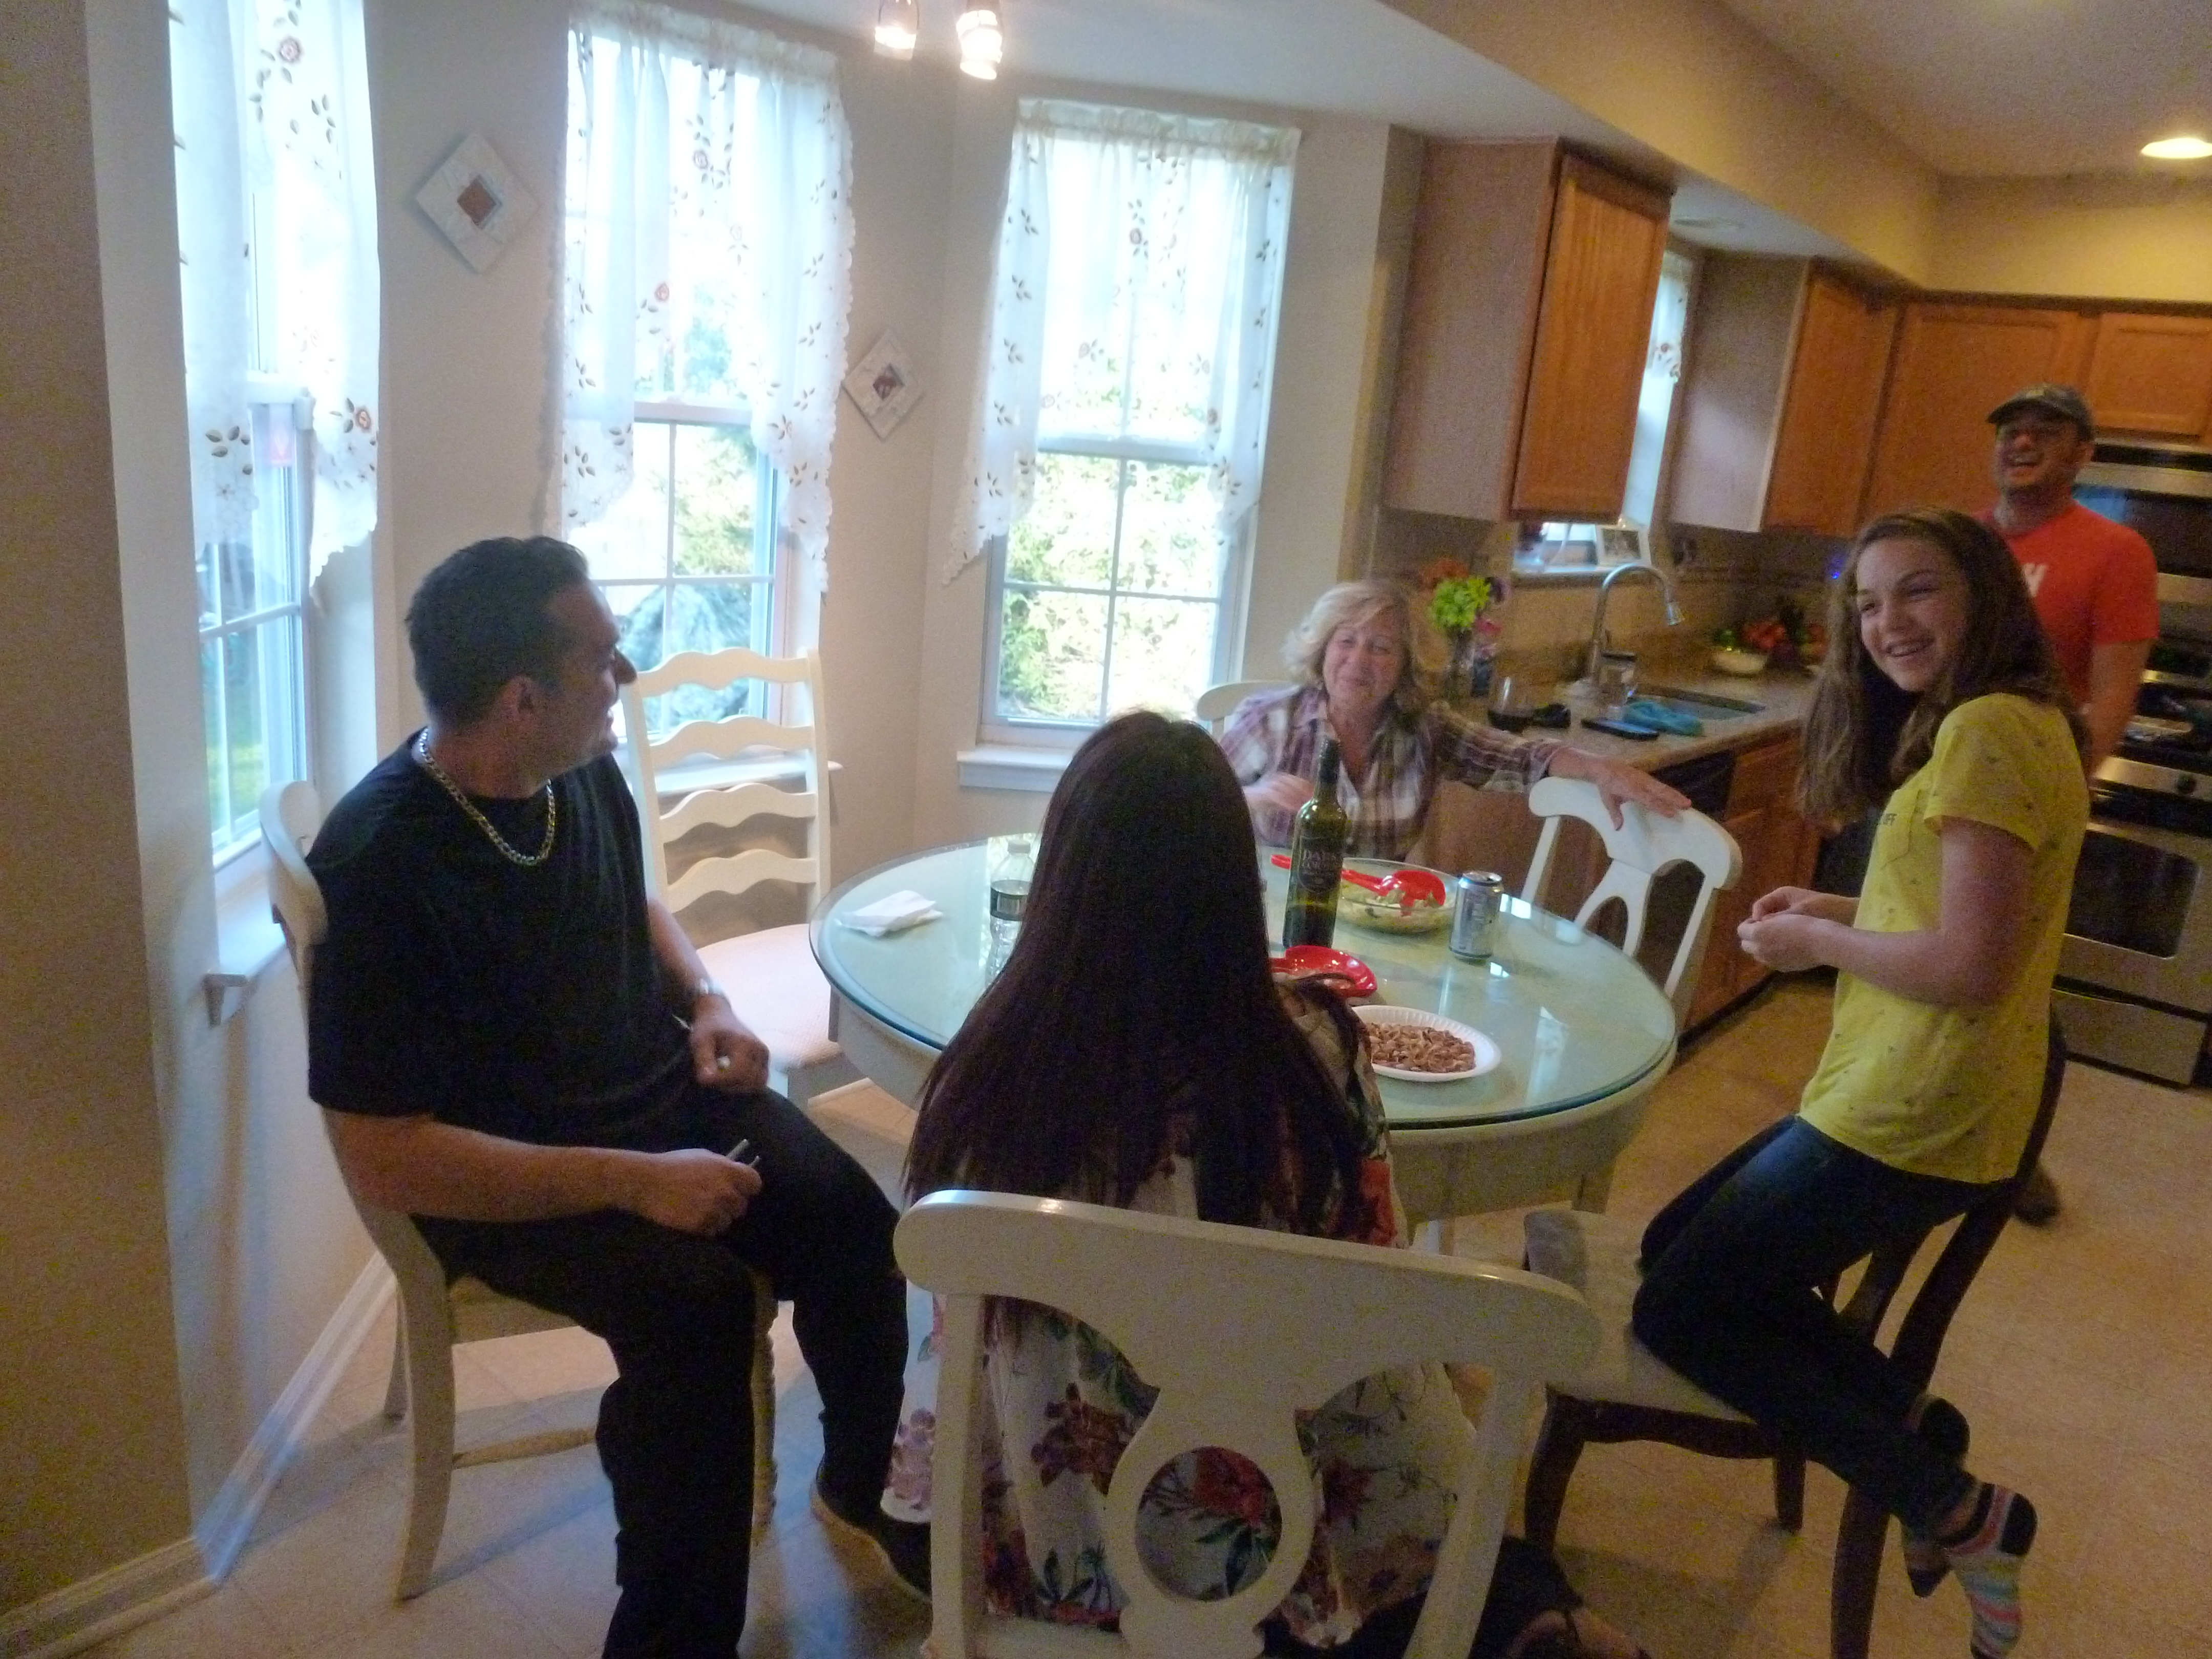
\includegraphics[width=0.45\linewidth,height=\textheight,keepaspectratio]{chapters/../images/P1020477.JPG}

}

\caption{``Look at yourselves!!!!'' --- September 2017}

\end{figure}%

\begin{figure}[H]

{\centering \includegraphics[width=0.45\linewidth,height=\textheight,keepaspectratio]{chapters/../images/family/DAD01.jpg}

}

\caption{Dad}

\end{figure}%

\begin{center}\rule{0.5\linewidth}{0.5pt}\end{center}

\emph{Three grandchildren. Two sons. Nearly sixty years of marriage. The
numbers tell the story of a man whose greatest achievement has always
been family.}

\chapter{``Love DAD''}\label{golden-years}

\emph{``Greg do you think you could purchase this pistol for me for
target practice, I would like some ammo as well. Let me know. Love
DAD''} --- Vic, age 75, shopping for an air pistol via email

\begin{tcolorbox}[enhanced jigsaw, left=2mm, leftrule=.75mm, opacityback=0, breakable, colframe=quarto-callout-note-color-frame, toprule=.15mm, bottomrule=.15mm, colback=white, arc=.35mm, rightrule=.15mm]
\begin{minipage}[t]{5.5mm}
\textcolor{quarto-callout-note-color}{\faInfo}
\end{minipage}%
\begin{minipage}[t]{\textwidth - 5.5mm}

\vspace{-3mm}\textbf{Soundtrack: Still Rocking at 80 (2000s--Today)}\vspace{3mm}

At 80, Vic's still going. Still shopping for air pistols, still hitting
AC, still signing every email ``Love DAD.'' Here's the soundtrack for a
man who earned every note:

\textbf{The Victory Lap} --- \emph{click any song to play}

\begin{itemize}
\tightlist
\item
  \href{https://www.youtube.com/watch?v=w019MzRosmk}{Frank Sinatra ---
  ``My Way''} \emph{(the only possible closer)}
\item
  \href{https://www.youtube.com/watch?v=1ERI1GoZ4NA}{Dean Martin ---
  ``Ain't That a Kick in the Head''}
\item
  \href{https://www.youtube.com/watch?v=M2-y-3a9RPg}{Bruce Springsteen
  --- ``Land of Hope and Dreams''} /
  \href{https://www.youtube.com/watch?v=tLeZ7EolBDE}{Bruce Springsteen
  --- ``No Surrender''}
\item
  \href{https://www.youtube.com/watch?v=1k8craCGpgs}{Journey --- ``Don't
  Stop Believin'''}
\item
  \href{https://www.youtube.com/watch?v=04854XqcfCY}{Queen --- ``We Are
  the Champions''}
\item
  \href{https://www.youtube.com/watch?v=ty1dwBCR6D0}{Neil Diamond ---
  ``Sweet Caroline''}
\item
  \href{https://www.youtube.com/watch?v=aZRn4auk4PQ}{Frank Sinatra ---
  ``Young at Heart''}
\item
  \href{https://www.youtube.com/watch?v=fMIJuuk1SFs}{Bob Seger ---
  ``Like a Rock''}
\item
  \href{https://www.youtube.com/watch?v=mTUhnIY3oRM}{The Four Seasons
  --- ``December, 1963 (Oh, What a Night)''}
\item
  \href{https://www.youtube.com/watch?v=mQIZ-Esbg_c}{Frank Sinatra ---
  ``The Best Is Yet to Come''}
\end{itemize}

\emph{What does Dad actually listen to these days? What station is the
car radio stuck on? What song does he sing in the shower?
\href{https://docs.google.com/forms/d/e/1FAIpQLSdpYXns7Zwutq6tDNp3BYU2HCPTHTgkdok6r9xWPpdXVPbvCQ/viewform}{Suggest
a song →} --- we'll add the best suggestions to the final playlist.}

\end{minipage}%
\end{tcolorbox}

\begin{tcolorbox}[enhanced jigsaw, toptitle=1mm, opacitybacktitle=0.6, leftrule=.75mm, breakable, toprule=.15mm, colbacktitle=quarto-callout-note-color!10!white, titlerule=0mm, left=2mm, opacityback=0, colframe=quarto-callout-note-color-frame, bottomtitle=1mm, title=\textcolor{quarto-callout-note-color}{\faInfo}\hspace{0.5em}{The World Since Retirement (2000--2026)}, arc=.35mm, colback=white, coltitle=black, rightrule=.15mm, bottomrule=.15mm]

\textbf{The broadest wavelet:} Vic retired into a century that started
with a shock. On \textbf{September 11, 2001} --- just a year into his
retirement --- the Twin Towers fell. From New Jersey's shoreline, you
could see the smoke rising from Lower Manhattan. The Pentagon was hit. A
plane went down in Pennsylvania. For a Vietnam veteran watching from
across the harbor, it was a new kind of war --- and this one was hitting
home.

Then came the wars that followed: Afghanistan (2001--2021), Iraq
(2003--2011). A Vietnam veteran watching a new generation of young
Americans shipped overseas. The financial crisis of \textbf{2008} ---
the Great Recession, the worst economic collapse since the Depression.
And then \textbf{COVID-19} in \textbf{2020} --- a pandemic that locked
the country down, separated families, and killed over a million
Americans. Vic was 74 when the pandemic hit. For a man whose life was
built on family proximity and gathering, the isolation was its own kind
of hardship.

\textbf{The Jersey wavelet:} \textbf{Superstorm Sandy} slammed into the
Jersey Shore on \textbf{October 29, 2012}, devastating the boardwalks,
beach towns, and communities that had been the Cicconetti family's world
for decades. Seaside Heights' boardwalk --- an icon of Shore culture ---
burned. Homes along the coast were destroyed. Point Pleasant, Avon,
Belmar --- all of them took hits. The Shore rebuilt, because that's what
the Shore does. But the families who lived through Sandy never forgot.

\textbf{The personal wavelet:} Through all of it --- 9/11, two wars, a
financial crisis, a superstorm, a pandemic --- Vic and Yvonne held
steady. The same partnership that had weathered Vietnam, career
building, and child-rearing now weathered the disruptions of the new
century. Still together. Still going to AC. Still signing every email
``Love DAD.''

\end{tcolorbox}

\section{Retirement, Jersey-Style}\label{retirement-jersey-style}

When Victor retired from public school administration in 2000, he didn't
slow down. He and Yvonne settled at \textbf{18 Waterview Ave in Neptune}
--- still Shore country, still close to the places where they'd raised
their family during the Shark River Hills (1980--1995) and Wall
(1995--2000) years. They lived in Neptune for two decades before moving
south in 2020 to \textbf{671 Cypress Point Drive at Blue Heron Pines} in
Egg Harbor City --- a golf community in Atlantic County, near the Pine
Barrens and the Shore, a quieter life but never a dull one.

Retirement for Vic has meant:

\begin{itemize}
\item
  \textbf{Atlantic City trips} --- multiple references in his emails to
  ``going to AC wed \& thurs.'' The casinos, the boardwalk, the
  restaurants. It's part of the NJ retirement lifestyle, and Vic and
  Yvonne are regulars. And AC has delivered its share of stories ---
  including the time Vic \textbf{shook hands with O.J. Simpson} at a
  fight in Atlantic City. Yes, \emph{that} O.J. The kind of random,
  only-in-AC celebrity encounter that becomes a family story told at
  every gathering for the next thirty years. Vic was there. O.J. was
  there. Hands were shaken. The family has opinions.
\item
  \textbf{Target practice at 75} --- In September 2021, Vic forwarded a
  Heartland America ad for a \textbf{Beeman Sportsman Deluxe Air Pistol}
  (\$49.99, .177 caliber) and asked Greg to order it. At seventy-five,
  Vic was still shooting, still active, still keeping his edge. The
  casual ``Love DAD'' sign-off on a request for ammunition is peak Vic.
\item
  \textbf{The daily briefing} --- Vic stays engaged with the world.
  \textbf{Fox News} is the soundtrack of the house. \textbf{Mark Levin}
  is the voice on the radio. He and Yvonne watch, listen, debate, and
  form opinions --- together, always together. They are not passive
  consumers. They are citizens who care deeply about the direction of
  their country, informed by a lifetime of experience that runs from
  Vietnam to the present.
\item
  \textbf{Wisdom curator} --- Vic forwards emails to his sons and
  brother-in-law Mike Hurley about life philosophy, faith, humor, and
  politics. He doesn't just consume this content --- he \emph{curates}
  it, selecting messages he believes carry real meaning and sharing them
  with the people he loves. The ``Gift of Time'' parable about Alexander
  the Great. Patriotic stories. Inspirational messages. Political
  commentary. Life lessons. Vic sees himself as passing wisdom --- and
  conviction --- to the next generation. The forward list is his
  broadcast network, and the signal is always the same: \emph{this
  matters, and I want you to see it}.
\end{itemize}

\section{The World That Changed Around
Him}\label{the-world-that-changed-around-him}

\begin{tcolorbox}[enhanced jigsaw, toptitle=1mm, opacitybacktitle=0.6, leftrule=.75mm, breakable, toprule=.15mm, colbacktitle=quarto-callout-note-color!10!white, titlerule=0mm, left=2mm, opacityback=0, colframe=quarto-callout-note-color-frame, bottomtitle=1mm, title=\textcolor{quarto-callout-note-color}{\faInfo}\hspace{0.5em}{80 Years of Everyday Things}, arc=.35mm, colback=white, coltitle=black, rightrule=.15mm, bottomrule=.15mm]

\textbf{Technology didn't just change in Vic's lifetime --- it changed
\emph{everything}, over and over, and he lived through every
transition:}

\textbf{In the kitchen:} The icebox became a refrigerator. The wringer
washer became an automatic. The dish-drying rack became a dishwasher.
The percolator became a Mr.~Coffee became a Keurig. Frozen TV dinners
arrived in 1954 and blew people's minds. The microwave oven --- military
technology repurposed for leftovers --- showed up in homes in the late
1970s and changed what ``cooking'' even meant.

\textbf{In the living room:} Three channels became cable (1980s) became
satellite (1990s) became streaming (2010s) became \emph{too many choices
to count}. The family gathered around \emph{one} television; now
everyone has a screen in their pocket. The VCR arrived and you could
record a show --- revolutionary. Then the DVD. Then the DVR. Then
Netflix made all of it obsolete. Vic has lived through every format of
recorded entertainment: vinyl records, 8-tracks, cassette tapes, CDs,
MP3s, and whatever his grandkids are using now.

\textbf{In communication:} The rotary phone (shared, on the wall, don't
tie up the line) became the push-button phone became the cordless phone
became the cell phone became the smartphone. The answering machine was a
miracle --- someone could leave a message when you weren't home! Then
voicemail. Then text messages. Then FaceTime. Vic's generation went from
\emph{waiting for the mail} to \emph{instant video calls with
grandchildren 200 miles away}. His email forwards --- the ones he
curates and sends to his sons every morning --- are his version of the
letters his grandparents sent from Italy. Same instinct. Different wire.

\textbf{In the car:} No seatbelts → seatbelts → airbags → backup cameras
→ cars that park themselves. Manual everything → power steering → cruise
control → GPS navigation. Vic learned to drive on a car you had to
\emph{crank}. His grandchildren will learn to drive on cars that drive
themselves.

\textbf{In school (where Vic spent his career):} Chalkboards → overhead
projectors → VCRs in the classroom → computer labs → laptops for every
student → AI tutors. Vic was \emph{ahead} of this curve --- writing
grants for Commodore computers in 1982 when most schools didn't even
have a computer room. He saw the future before the district budget
caught up.

The man who was born into a world of rotary phones and iceboxes now
lives in a world of smartphones and AI. And he adapted to every single
transition --- not because he's a technologist, but because he's a man
who refuses to be left behind.

\end{tcolorbox}

\section{``Glue Fingers'' and the Old
Crew}\label{glue-fingers-and-the-old-crew}

Some identities don't fade. Somewhere in a box or a scrapbook, there's
an old newspaper clipping where a young Victor Cicconetti earned the
nickname \textbf{``Glue Fingers Cicconetti''} --- a receiver who didn't
drop the ball. That was high school football in Bayonne, where Friday
nights under the lights were the center of the social universe and a
good nickname followed you for life.

In his later years, Vic has enjoyed \textbf{periodic gatherings with his
old high school football buddies} --- the guys who blocked for him, ran
alongside him, and shared the locker room camaraderie that becomes,
decades later, one of the purest forms of friendship a man can have. No
pretense. No agenda. Just men who knew each other when they were
seventeen and still show up for each other at seventy-nine.

The football brotherhood and the veteran brotherhood overlap in Vic's
life --- both are groups of men who went through something intense
together and never let go of the bond. ``Glue Fingers'' caught passes in
Bayonne. Then he caught wounded soldiers in medevac helicopters. Then he
caught students who were falling through the cracks. The hands never
stopped reaching.

\begin{tcolorbox}[enhanced jigsaw, toptitle=1mm, opacitybacktitle=0.6, leftrule=.75mm, breakable, toprule=.15mm, colbacktitle=quarto-callout-note-color!10!white, titlerule=0mm, left=2mm, opacityback=0, colframe=quarto-callout-note-color-frame, bottomtitle=1mm, title=\textcolor{quarto-callout-note-color}{\faInfo}\hspace{0.5em}{Check Our Work --- Football}, arc=.35mm, colback=white, coltitle=black, rightrule=.15mm, bottomrule=.15mm]

\begin{longtable}[]{@{}llccc@{}}
\toprule\noalign{}
\# & We wrote\ldots{} & TRUE & FALSE & I DON'T KNOW \\
\midrule\noalign{}
\endhead
\bottomrule\noalign{}
\endlastfoot
1 & Vic played high school football in Bayonne & & & \\
2 & He was nicknamed ``Glue Fingers Cicconetti'' & & & \\
3 & He still gathers with old football friends & & & \\
\end{longtable}

\textbf{What school? What position? What years? Do you still have the
newspaper clipping?}

\hfill\break

\end{tcolorbox}

\section{The Shore Pilgrimage}\label{the-shore-pilgrimage}

Even after moving south to Blue Heron Pines in 2020, Vic and Yvonne
never let go of the Shore. At 79, they still make the pilgrimage ---
north on the Parkway to the places where they raised their family, where
the kids grew up, where the memories live.

The destinations are always the same, because that's the point:

\begin{itemize}
\tightlist
\item
  \textbf{Avon-by-the-Sea} --- the quiet beach town with the Victorian
  boardwalk, where the ocean is the attraction and the crowds stay away.
  Not Seaside Heights. Not Wildwood. \emph{Avon.} That tells you
  everything about Vic and Yvonne's taste.
\item
  \textbf{Point Pleasant Beach} --- the boardwalk, Jenkinson's, the
  fishing pier, the arcades where the grandkids play the same games the
  kids played thirty years ago. Shore culture passed down.
\item
  \textbf{Pete \& Elda's} --- the thin-crust pizza institution in
  Neptune City, open since 1956. Every Shore family has a Pete \& Elda's
  booth that feels like theirs. The Cicconettis' is no different.
\item
  \textbf{Kelly's Tavern} --- cold drinks, familiar faces, the kind of
  place where Vic walks in and someone says ``hey, Vic.''
\end{itemize}

These aren't restaurants and beaches. They're \emph{landmarks on the map
of a life}. The Shark River Hills years (1980--1995), the Wall years
(1995--2000), the Neptune years (2000--2020) --- decades of Shore living
compressed into an afternoon drive and a pizza that tastes like 1985.

That they still make this trip, into their late seventies and now
approaching eighty --- that's not nostalgia. That's identity. The Jersey
Shore isn't where Vic vacations. It's where Vic \emph{is}.

\begin{tcolorbox}[enhanced jigsaw, toptitle=1mm, opacitybacktitle=0.6, leftrule=.75mm, breakable, toprule=.15mm, colbacktitle=quarto-callout-note-color!10!white, titlerule=0mm, left=2mm, opacityback=0, colframe=quarto-callout-note-color-frame, bottomtitle=1mm, title=\textcolor{quarto-callout-note-color}{\faInfo}\hspace{0.5em}{Map: The Shore --- Then and Now}, arc=.35mm, colback=white, coltitle=black, rightrule=.15mm, bottomrule=.15mm]

Four decades of Shore living: Shark River Hills (1980--1995) → Wall
(1995--2000) → Neptune (2000--2020) → Blue Heron Pines (2020--present).
Plus the landmarks that never change: Pete \& Elda's, Point Pleasant,
Avon-by-the-Sea.

\emph{Interactive map available in the online version.}

\end{tcolorbox}

\begin{tcolorbox}[enhanced jigsaw, toptitle=1mm, opacitybacktitle=0.6, leftrule=.75mm, breakable, toprule=.15mm, colbacktitle=quarto-callout-tip-color!10!white, titlerule=0mm, left=2mm, opacityback=0, colframe=quarto-callout-tip-color-frame, bottomtitle=1mm, title=\textcolor{quarto-callout-tip-color}{\faLightbulb}\hspace{0.5em}{Tell Us a Shore Story}, arc=.35mm, colback=white, coltitle=black, rightrule=.15mm, bottomrule=.15mm]

\textbf{Everyone:} What's the definitive Cicconetti Shore story? The
beach day that went sideways? The Pete \& Elda's night that turned
legendary? The time at Kelly's that nobody's allowed to talk about? The
boardwalk game somebody FINALLY won after twenty years of trying?

\textbf{Dad \& Mom:} Is there a beach, a bench, a spot on the boardwalk
that's \emph{yours}? The place you go when it's just the two of you?

\end{tcolorbox}

\section{How Vic Communicates}\label{how-vic-communicates}

Victor's email style is a window into his personality:

\begin{longtable}[]{@{}
  >{\raggedright\arraybackslash}p{(\linewidth - 2\tabcolsep) * \real{0.5000}}
  >{\raggedright\arraybackslash}p{(\linewidth - 2\tabcolsep) * \real{0.5000}}@{}}
\toprule\noalign{}
\begin{minipage}[b]{\linewidth}\raggedright
Pattern
\end{minipage} & \begin{minipage}[b]{\linewidth}\raggedright
Example
\end{minipage} \\
\midrule\noalign{}
\endhead
\bottomrule\noalign{}
\endlastfoot
\textbf{Brief subject-as-message} & Subject: ``How you doing?'' Body:
empty \\
\textbf{Emotional milestone responses} & ``Dearest Son, I hope you can
take a long breath and exhale!!!!'' \\
\textbf{The check-in} & ``What's happening? Did you hear from them? We
are going to AC wed \& thurs be back Fri pm. Call you later. Dad'' \\
\textbf{Proud grandpa} & ``Look at yourselves!!!!'' (with photo, no body
text) \\
\textbf{Consistent sign-off} & ``Love DAD'' --- every single time \\
\textbf{Consistent greeting} & ``Dearest Son'' or ``Dearest Greg'' \\
\end{longtable}

The man who grew up before email, before texting, before social media
--- he adapted to the digital age on his own terms. Brief. Warm.
Consistent. And always ending with love.

\begin{tcolorbox}[enhanced jigsaw, toptitle=1mm, opacitybacktitle=0.6, leftrule=.75mm, breakable, toprule=.15mm, colbacktitle=quarto-callout-note-color!10!white, titlerule=0mm, left=2mm, opacityback=0, colframe=quarto-callout-note-color-frame, bottomtitle=1mm, title=\textcolor{quarto-callout-note-color}{\faInfo}\hspace{0.5em}{Check Our Work --- The Golden Years}, arc=.35mm, colback=white, coltitle=black, rightrule=.15mm, bottomrule=.15mm]

\begin{longtable}[]{@{}
  >{\raggedright\arraybackslash}p{(\linewidth - 8\tabcolsep) * \real{0.0732}}
  >{\raggedright\arraybackslash}p{(\linewidth - 8\tabcolsep) * \real{0.2683}}
  >{\centering\arraybackslash}p{(\linewidth - 8\tabcolsep) * \real{0.1463}}
  >{\centering\arraybackslash}p{(\linewidth - 8\tabcolsep) * \real{0.1707}}
  >{\centering\arraybackslash}p{(\linewidth - 8\tabcolsep) * \real{0.3415}}@{}}
\toprule\noalign{}
\begin{minipage}[b]{\linewidth}\raggedright
\#
\end{minipage} & \begin{minipage}[b]{\linewidth}\raggedright
We wrote\ldots{}
\end{minipage} & \begin{minipage}[b]{\linewidth}\centering
TRUE
\end{minipage} & \begin{minipage}[b]{\linewidth}\centering
FALSE
\end{minipage} & \begin{minipage}[b]{\linewidth}\centering
I DON'T KNOW
\end{minipage} \\
\midrule\noalign{}
\endhead
\bottomrule\noalign{}
\endlastfoot
1 & You live at Blue Heron Pines in Egg Harbor City (since 2020); before
that, Neptune (2000--2020) & & & \\
2 & You're regulars at Atlantic City & & & \\
3 & At 75, Vic asked Greg to order him an air pistol & & & \\
4 & After the 75th birthday party, Vic walked around the house laughing
& & & \\
\end{longtable}

\textbf{Anything wrong? Fill in what we missed:}

\hfill\break

\end{tcolorbox}

\begin{tcolorbox}[enhanced jigsaw, toptitle=1mm, opacitybacktitle=0.6, leftrule=.75mm, breakable, toprule=.15mm, colbacktitle=quarto-callout-tip-color!10!white, titlerule=0mm, left=2mm, opacityback=0, colframe=quarto-callout-tip-color-frame, bottomtitle=1mm, title=\textcolor{quarto-callout-tip-color}{\faLightbulb}\hspace{0.5em}{Tell Us a Story}, arc=.35mm, colback=white, coltitle=black, rightrule=.15mm, bottomrule=.15mm]

\textbf{Dad:} Do you have an Atlantic City system? Be honest --- slots,
poker, blackjack, craps? What's your biggest win? And what about the one
you probably shouldn't tell us about?

\textbf{Mom:} What's the thing Dad does in retirement that drives you
absolutely crazy? And what's the thing he does that still makes you fall
in love with him all over again?

\end{tcolorbox}

\section{Faith}\label{faith}

Vic's faith threads through everything he does. Not the quiet, private
kind that stays in the pew. The \emph{Vic} kind --- persistent, vocal,
and coming at you whether you asked for it or not.

\begin{quote}
``The Lord has blessed you once more.''
\end{quote}

That's how he frames milestones --- as blessings, not just achievements.
Every email, every phone call, every milestone: \emph{pray about it}. A
grandchild's graduation? \emph{The Lord has blessed you}. A new job?
\emph{God is good}. A rough patch? \emph{Have you prayed on it?}

Here's the thing: the Cicconetti family stopped going to church decades
ago. After Rich finished grammar school, they were done with the
monotony of Catholic Mass. The whole family moved on. And then Vic found
his Baptist church, did his deep dive into scripture, and came out the
other side as the family's \textbf{permanent, unsolicited spiritual
advisor}.

The joke in the family --- and it \emph{is} a joke, told with love ---
goes like this:

\emph{``Did Dad have a few drinks and corner you to talk about the Bible
again?''}

Because that's what happens. A family gathering. A barbecue. A holiday.
Vic has a couple of drinks, and suddenly you're getting a one-on-one
about prayer, about gratitude, about what the scriptures say about
perseverance. He doesn't do it from a pulpit. He does it from a lawn
chair, or the kitchen counter, or the driver's seat on the way to Point
Pleasant. He persists through resistance. He \emph{always} persists
through resistance.

Nobody in the family goes to church anymore. But Vic never stopped being
the voice that says: \textbf{pray}. Pray when things are good. Pray when
things are bad. Pray when you don't feel like it. \emph{Especially} when
you don't feel like it.

It's not performative. It's not preachy --- well, it's a \emph{little}
preachy. But it's real. The man who read the Bible cover to cover, who
led youth groups, who joined a Baptist church to challenge himself ---
that man didn't stop when the formal churchgoing stopped. He just moved
the ministry to the dinner table, the phone call, the email forward. His
congregation is his family, and his sermons never end.

The Catholic boy from Bayonne, who married at Assumption Church, who
left the monotony of Mass, who walked into a Baptist church, who read
the whole book, who now signs his emails with ``God bless'' and calls
his sons to tell them to pray --- that man's faith isn't a Sunday habit.
It's a Tuesday habit. A Wednesday habit. An every-damn-day habit. And if
you're within earshot after he's had a glass of wine? You're going to
hear about it.

\section{The Walk-Around-the-House
Laugh}\label{the-walk-around-the-house-laugh}

After his 75th birthday party in 2021, Vic sent a thank-you email to
Greg's family that captures something essential about who he is:

\begin{quote}
``I am still laughing at your antics on the video. I can be walking
around the house and suddenly I think of Greg and Val and man I start
smiling then laughing.''
\end{quote}

Picture it: Vic, alone in the house, walking from room to room, and
suddenly --- a memory from the party hits him, and he laughs out loud.
Not once, but again and again, days later. This is a man who holds joy
close. Who lets the good moments replay. Who walks around his house and
laughs at the love of his family.

That image --- Vic wandering the house, suddenly breaking into laughter
--- belongs in any portrait of who this man really is.

\begin{tcolorbox}[enhanced jigsaw, toptitle=1mm, opacitybacktitle=0.6, leftrule=.75mm, breakable, toprule=.15mm, colbacktitle=quarto-callout-note-color!10!white, titlerule=0mm, left=2mm, opacityback=0, colframe=quarto-callout-note-color-frame, bottomtitle=1mm, title=\textcolor{quarto-callout-note-color}{\faInfo}\hspace{0.5em}{America's Changing Relationship with Marijuana}, arc=.35mm, colback=white, coltitle=black, rightrule=.15mm, bottomrule=.15mm]

\textbf{The broadest wavelet:} Few substances trace the arc of American
culture as cleanly as marijuana. When Vic was growing up in the 1950s,
cannabis was the stuff of \emph{Reefer Madness} propaganda --- a
Schedule I narcotic lumped with heroin, a moral panic in plant form. By
the time he was in Vietnam, it was everywhere among the troops --- a
coping mechanism for the uncopeable.

\begin{itemize}
\tightlist
\item
  \textbf{1970:} Nixon signed the Controlled Substances Act, classifying
  marijuana as Schedule I --- ``no accepted medical use, high potential
  for abuse.'' The War on Drugs began.
\item
  \textbf{1980s--90s:} Reagan and Clinton escalated enforcement. ``Just
  Say No.'' Mandatory minimums. By 1997, nearly \textbf{700,000
  Americans} were arrested annually for marijuana offenses --- more than
  for all violent crimes combined.
\item
  \textbf{1996:} California passed \textbf{Proposition 215}, the first
  medical marijuana law. The dam cracked.
\item
  \textbf{2012:} Colorado and Washington became the first states to
  legalize recreational use.
\item
  \textbf{2020:} New Jersey voters approved \textbf{Question 1},
  legalizing recreational marijuana. Vic's home state.
\item
  \textbf{2024:} By now, 24 states plus DC have legalized recreational
  use. The substance that could get you prison time when Vic was raising
  his family is now sold in storefronts down the road from his house.
\end{itemize}

The generation that grew up with ``Just Say No'' is now the generation
buying edibles at a dispensary. The country didn't just change its laws
--- it changed its entire moral framework around a plant. For a man who
has lived through Vietnam, Watergate, the War on Drugs, and legalization
--- all in one lifetime --- the whiplash is its own kind of American
experience.

\end{tcolorbox}

\section{He Won't Back Down}\label{he-wont-back-down}

At eighty, Vic is still Vic. He still goes to AC. He still drives to
Point Pleasant. He still forwards emails at 6 AM. He still walks around
the house laughing at memories of his family. He still signs every
message ``Love DAD.''

The man who flew medevac missions through combat zones, who walked into
a student walkout and led a prayer, who bumped a rifle score by a point
to get his kid across the line --- that man has never let anything have
the last word.

He watched his own father die at fifty-five. He joined a Baptist church
to break the cycles he didn't want to repeat. He read the Bible cover to
cover. He ran. He pushed everyone around him to be better. And he kept
going.

Tom Petty wrote it: \emph{I won't back down.} The Traveling Wilburys
sang it: \emph{It's all right, even if you're old and gray.} Sinatra
closed every show the same way: \emph{I did it my way.}

Vic lives all three.

\begin{tcolorbox}[enhanced jigsaw, toptitle=1mm, opacitybacktitle=0.6, leftrule=.75mm, breakable, toprule=.15mm, colbacktitle=quarto-callout-note-color!10!white, titlerule=0mm, left=2mm, opacityback=0, colframe=quarto-callout-note-color-frame, bottomtitle=1mm, title=\textcolor{quarto-callout-note-color}{\faInfo}\hspace{0.5em}{Your Turn --- Dad}, arc=.35mm, colback=white, coltitle=black, rightrule=.15mm, bottomrule=.15mm]

We wrote this chapter mostly from your emails. But we want the rest of
the picture.

\begin{itemize}
\tightlist
\item
  What does a normal Tuesday look like for you?
\item
  Which casino is your casino? Do you have a system?
\item
  Are you still shooting? Still doing target practice?
\item
  What do you watch? What do you read? What music?
\item
  What makes you laugh the hardest?
\item
  What's the thing you do that drives Mom crazy but she secretly loves?
\end{itemize}

\textbf{Mom:} What's the thing \emph{he} does that drives you crazy? And
what's the thing about him that still makes you smile after all these
years?

\textbf{Everyone else:} What's the funniest recent Vic story? The most
recent time he made you laugh until you cried?

\end{tcolorbox}

\section*{Photo Gallery: The Golden
Years}\label{photo-gallery-the-golden-years}
\addcontentsline{toc}{section}{Photo Gallery: The Golden Years}

\markright{Photo Gallery: The Golden Years}

\begin{figure}[H]

{\centering \includegraphics[width=0.45\linewidth,height=\textheight,keepaspectratio]{chapters/../images/recent/DAD02.jpg}

}

\caption{Dad}

\end{figure}%

\begin{figure}[H]

{\centering \includegraphics[width=0.45\linewidth,height=\textheight,keepaspectratio]{chapters/../images/recent/DSC00014.JPG}

}

\caption{Family event, 2000s}

\end{figure}%

\begin{figure}[H]

{\centering \includegraphics[width=0.45\linewidth,height=\textheight,keepaspectratio]{chapters/../images/recent/DSC01904.JPG}

}

\caption{The Shore, always the Shore}

\end{figure}%

\begin{figure}[H]

{\centering \includegraphics[width=0.45\linewidth,height=\textheight,keepaspectratio]{chapters/../images/recent/Picture 352.jpg}

}

\caption{Still going strong}

\end{figure}%

\begin{figure}[H]

{\centering \includegraphics[width=0.45\linewidth,height=\textheight,keepaspectratio]{chapters/../images/recent/rich and greg.JPG}

}

\caption{Rich \& Greg}

\end{figure}%

\begin{figure}[H]

{\centering \includegraphics[width=0.45\linewidth,height=\textheight,keepaspectratio]{chapters/../images/recent/cicc.jpg}

}

\caption{Vic}

\end{figure}%

\begin{center}\rule{0.5\linewidth}{0.5pt}\end{center}

\emph{At eighty, Victor Cicconetti is still shopping for air pistols,
still going to Atlantic City, still forwarding wisdom to his sons, and
still walking around the house laughing at memories of his family. He
did it his way. And the best is yet to come.}

{Love DAD}

\part{Part IV: Celebration}

\chapter{In Their Own Words}\label{voices}

\emph{``sshhh its a surprise'' --- Subject line of Greg's invitation to
the family to contribute tribute messages, February 6, 2026}

\section{A Family Tribute}\label{a-family-tribute}

On February 6, 2026, Greg sent an email with the subject line
\textbf{``sshhh its a surprise''} to the inner circle: Yvonne, Rich,
Kathy Pacifico, AJ, Ellie, Jen, Mike Hurley (both addresses), and
Valerie \& Frank Elia. The invitation: contribute a message for Dad's
80th birthday tribute book.

This chapter belongs to the family. Each person who knows and loves
Victor has their own story to tell --- their own memory, their own
moment, their own way of saying what he means to them.

\begin{tcolorbox}[enhanced jigsaw, toptitle=1mm, opacitybacktitle=0.6, leftrule=.75mm, breakable, toprule=.15mm, colbacktitle=quarto-callout-important-color!10!white, titlerule=0mm, left=2mm, opacityback=0, colframe=quarto-callout-important-color-frame, bottomtitle=1mm, title=\textcolor{quarto-callout-important-color}{\faExclamation}\hspace{0.5em}{Add Your Message}, arc=.35mm, colback=white, coltitle=black, rightrule=.15mm, bottomrule=.15mm]

\textbf{Want to contribute online?} Use the tribute form --- type as
much or as little as you want. You can even upload a photo.

\href{https://docs.google.com/forms/d/e/1FAIpQLSdpYXns7Zwutq6tDNp3BYU2HCPTHTgkdok6r9xWPpdXVPbvCQ/viewform}{Write
Your Message for Dad}

\end{tcolorbox}

\begin{center}\rule{0.5\linewidth}{0.5pt}\end{center}

\section*{From Yvonne}\label{from-yvonne}
\addcontentsline{toc}{section}{From Yvonne}

\markright{From Yvonne}

\begin{tcolorbox}[enhanced jigsaw, toptitle=1mm, opacitybacktitle=0.6, leftrule=.75mm, breakable, toprule=.15mm, colbacktitle=quarto-callout-tip-color!10!white, titlerule=0mm, left=2mm, opacityback=0, colframe=quarto-callout-tip-color-frame, bottomtitle=1mm, title=\textcolor{quarto-callout-tip-color}{\faLightbulb}\hspace{0.5em}{Tell Us a Story}, arc=.35mm, colback=white, coltitle=black, rightrule=.15mm, bottomrule=.15mm]

\textbf{Mom:} What's the thing about Dad that nobody else sees? The
private Vic --- the one who exists when it's just the two of you? What
do you want to say to him after almost sixty years together?

\end{tcolorbox}

\textbf{{[}AWAITING CONTRIBUTION{]}} --- Yvonne's message for Victor's
80th birthday.

\begin{center}\rule{0.5\linewidth}{0.5pt}\end{center}

\section*{From Rich}\label{from-rich}
\addcontentsline{toc}{section}{From Rich}

\markright{From Rich}

\begin{tcolorbox}[enhanced jigsaw, toptitle=1mm, opacitybacktitle=0.6, leftrule=.75mm, breakable, toprule=.15mm, colbacktitle=quarto-callout-tip-color!10!white, titlerule=0mm, left=2mm, opacityback=0, colframe=quarto-callout-tip-color-frame, bottomtitle=1mm, title=\textcolor{quarto-callout-tip-color}{\faLightbulb}\hspace{0.5em}{Tell Us a Story}, arc=.35mm, colback=white, coltitle=black, rightrule=.15mm, bottomrule=.15mm]

\textbf{Rich:} What's your earliest memory of Dad? The first one, no
matter how fuzzy. And what's the thing he taught you --- not in a
lesson, but just by being him --- that you carry with you every day?

\end{tcolorbox}

\textbf{{[}AWAITING CONTRIBUTION{]}} --- Rich's message for his father.

\begin{center}\rule{0.5\linewidth}{0.5pt}\end{center}

\section*{From Greg}\label{from-greg}
\addcontentsline{toc}{section}{From Greg}

\markright{From Greg}

\begin{tcolorbox}[enhanced jigsaw, toptitle=1mm, opacitybacktitle=0.6, leftrule=.75mm, breakable, toprule=.15mm, colbacktitle=quarto-callout-tip-color!10!white, titlerule=0mm, left=2mm, opacityback=0, colframe=quarto-callout-tip-color-frame, bottomtitle=1mm, title=\textcolor{quarto-callout-tip-color}{\faLightbulb}\hspace{0.5em}{Tell Us a Story}, arc=.35mm, colback=white, coltitle=black, rightrule=.15mm, bottomrule=.15mm]

\textbf{Greg:} You've been building this book. You know the facts better
than anyone. Now forget the facts --- what's the \emph{feeling}? What
does ``Love DAD'' at the end of every email actually mean to you?

\end{tcolorbox}

\textbf{{[}AWAITING CONTRIBUTION{]}} --- Greg's message for his father.

\begin{center}\rule{0.5\linewidth}{0.5pt}\end{center}

\section*{From the Grandchildren}\label{from-the-grandchildren}
\addcontentsline{toc}{section}{From the Grandchildren}

\markright{From the Grandchildren}

\begin{tcolorbox}[enhanced jigsaw, toptitle=1mm, opacitybacktitle=0.6, leftrule=.75mm, breakable, toprule=.15mm, colbacktitle=quarto-callout-tip-color!10!white, titlerule=0mm, left=2mm, opacityback=0, colframe=quarto-callout-tip-color-frame, bottomtitle=1mm, title=\textcolor{quarto-callout-tip-color}{\faLightbulb}\hspace{0.5em}{Tell Us a Story}, arc=.35mm, colback=white, coltitle=black, rightrule=.15mm, bottomrule=.15mm]

\textbf{Grandkids:} Don't overthink this. Just answer one question:
\emph{What's the thing Grandpa does that always makes you smile?} Maybe
it's the way he laughs. Maybe it's something he says every single time.
Maybe it's a face he makes. Whatever it is --- write it down. Even one
sentence is perfect.

\end{tcolorbox}

\textbf{{[}AWAITING CONTRIBUTIONS{]}} --- Messages from Victor's three
grandchildren: Ellie, Anthony, and Richy.

\begin{center}\rule{0.5\linewidth}{0.5pt}\end{center}

\section*{From the Extended Family}\label{from-the-extended-family}
\addcontentsline{toc}{section}{From the Extended Family}

\markright{From the Extended Family}

Kathy Pacifico, Mike Hurley, Valerie \& Frank Elia --- and anyone else
who wants to share a word.

\begin{tcolorbox}[enhanced jigsaw, toptitle=1mm, opacitybacktitle=0.6, leftrule=.75mm, breakable, toprule=.15mm, colbacktitle=quarto-callout-tip-color!10!white, titlerule=0mm, left=2mm, opacityback=0, colframe=quarto-callout-tip-color-frame, bottomtitle=1mm, title=\textcolor{quarto-callout-tip-color}{\faLightbulb}\hspace{0.5em}{Tell Us a Story}, arc=.35mm, colback=white, coltitle=black, rightrule=.15mm, bottomrule=.15mm]

\textbf{Kathy:} You organized the 75th. What do you know about pulling
off a Cicconetti celebration that the rest of us should know? What was
the moment from that party that sticks with you?

\textbf{Valerie \& Frank Elia:} What's your favorite Vic-and-Yvonne
story from the Elia side of the family?

\end{tcolorbox}

\textbf{{[}AWAITING CONTRIBUTIONS{]}} --- Messages from the extended
family.

\begin{center}\rule{0.5\linewidth}{0.5pt}\end{center}

\section*{From Fellow Veterans}\label{from-fellow-veterans}
\addcontentsline{toc}{section}{From Fellow Veterans}

\markright{From Fellow Veterans}

The brotherhood of VVA Chapter 12 --- Leon, David Connelly, Larry
Messina, and others from Vic's forward network.

\begin{tcolorbox}[enhanced jigsaw, toptitle=1mm, opacitybacktitle=0.6, leftrule=.75mm, breakable, toprule=.15mm, colbacktitle=quarto-callout-tip-color!10!white, titlerule=0mm, left=2mm, opacityback=0, colframe=quarto-callout-tip-color-frame, bottomtitle=1mm, title=\textcolor{quarto-callout-tip-color}{\faLightbulb}\hspace{0.5em}{Tell Us a Story}, arc=.35mm, colback=white, coltitle=black, rightrule=.15mm, bottomrule=.15mm]

\textbf{Veterans:} Vic doesn't know about this book. Here's your chance
to say something about him behind his back --- the good kind. What kind
of leader was he at Chapter 12? What did the chapter mean to the men who
showed up? What's the Vic story you wish everyone knew?

\end{tcolorbox}

\textbf{{[}AWAITING CONTRIBUTIONS{]}} --- Messages from fellow veterans
and friends.

\begin{center}\rule{0.5\linewidth}{0.5pt}\end{center}

\emph{This chapter will be filled with the voices of the people who know
Victor best. Their words will be the heart of this book.}

\begin{center}\rule{0.5\linewidth}{0.5pt}\end{center}

\section*{Submit Your Tribute Online}\label{submit-your-tribute-online}
\addcontentsline{toc}{section}{Submit Your Tribute Online}

\markright{Submit Your Tribute Online}

Loading form\ldots{}

\chapter{Happy 80th, Dad}\label{happy-80th}

\emph{``An American story.'' --- Red Bank Register, 1987}

\section{A Life Well Lived}\label{a-life-well-lived}

As Victor R. Cicconetti turns eighty, the measure of his life is not
found in any single achievement --- but in the remarkable breadth of
what he has given.

\textbf{To his country:} Four years of service as an Air Force medic,
flying into danger to bring wounded servicemembers home from Vietnam.

\textbf{To his students:} Decades of dedication in New Jersey's public
schools, shaping young lives from Long Branch to Asbury Park --- the
``Man with Many Missions.''

\textbf{To his fellow veterans:} A founding voice for Vietnam Veterans
of America Chapter 12, ensuring that those who served were never
forgotten. Life memberships in the VA and the DAV. A lifetime of showing
up.

\textbf{To his family:} Nearly sixty years of partnership with Yvonne.
Two sons. Three grandchildren. A home built on love, food,
Italian-American tradition, and the two most important words in his
vocabulary: {Love DAD}.

\textbf{To his community:} Entrepreneurship, education, advocacy, and
the quiet daily work of being a good neighbor, a good friend, and a good
man.

\section{The Story So Far}\label{the-story-so-far}

Victor's story is --- as a New Jersey newspaper once wrote --- ``an
American story.'' It is the story of Italian immigrants who left the
mountains of Abruzzo for the streets of Bayonne. It is the story of a
young man who answered his country's call at nineteen and flew medevac
missions in Vietnam. It is the story of a veteran who came home and
built a career helping young people. It is the story of a husband, a
father, and a grandfather who signs every email with love.

From Collepietro to Bayonne. From the Air Force to the classroom. From
the classroom to the restaurant to the VVA hall. From one generation to
the next --- and the next --- and the next.

\begin{tcolorbox}[enhanced jigsaw, toptitle=1mm, opacitybacktitle=0.6, leftrule=.75mm, breakable, toprule=.15mm, colbacktitle=quarto-callout-tip-color!10!white, titlerule=0mm, left=2mm, opacityback=0, colframe=quarto-callout-tip-color-frame, bottomtitle=1mm, title=\textcolor{quarto-callout-tip-color}{\faLightbulb}\hspace{0.5em}{One Last Story}, arc=.35mm, colback=white, coltitle=black, rightrule=.15mm, bottomrule=.15mm]

\textbf{Everyone:} If you could describe Vic in exactly three words ---
just three --- what would they be?

And one more: What's the thing about Victor Cicconetti that you want his
great-grandchildren to know someday?

\end{tcolorbox}

\section{How This Book Was Made}\label{how-this-book-was-made}

Dad, you might be wondering: \emph{how did they put all this together?}

Here's the short version: \textbf{Greg sat at his computer and told
stories about you.} That's really it. He talked about growing up in
Shark River Hills, about your career at Long Branch, about the
restaurant, the parades, the Baptist church, the Shore trips, the emails
you send at 6 AM. Everything he remembered. Everything the family
remembers.

But he didn't type the book himself. He had help from a new kind of tool
--- an \textbf{artificial intelligence assistant} called
\textbf{Claude}. Think of it like this: if Greg hired a really good
writer to help him organize his thoughts, that's basically what
happened. Except the writer lives inside the computer.

Here's how the process worked:

\includegraphics[width=8in,height=21.29in]{chapters/ch10-happy-80th_files/figure-latex/mermaid-figure-1.png}

How This Book Came Together

\textbf{In plain English:}

\begin{enumerate}
\def\labelenumi{\arabic{enumi}.}
\item
  \textbf{Greg talked.} He sat down over several sessions and told the
  story of your life --- the parts he knows, the parts the family knows,
  the parts that come from your emails and photos and the stories you've
  told a hundred times at the dinner table.
\item
  \textbf{The computer organized it.} Claude took those stories and
  arranged them into chapters, added historical context (what was
  happening in the country during each era of your life), found the
  right music for each era, and made it look nice on the screen.
\item
  \textbf{Greg checked everything.} Every single fact, every story,
  every detail --- Greg read it and either approved it, corrected it, or
  said ``that's not right, here's what really happened.'' The AI doesn't
  know your life --- \emph{Greg does}. Claude is the pen. Greg is the
  author.
\item
  \textbf{The family fills in the gaps.} That's what those ``Check Our
  Work'' boxes are for --- so you, Mom, Rich, Ellie, Anthony, and Richy
  can tell us what we got right, what we got wrong, and what stories
  we're missing.
\item
  \textbf{It became this website.} The book you're reading is a website
  that works on your computer, your phone, or a tablet. It's not printed
  (yet --- we might make a printed version too). The music links play
  real songs. The photos are from the family collection.
\end{enumerate}

\textbf{What Greg actually did:} He's the architect of this whole thing.
He decided what the book should be. He chose the structure. He told the
stories. He picked the music. He reviewed every word. He's the one who
knows that ``Glue Fingers'' was your football nickname and that you
shook O.J.'s hand in AC and that you read the Bible cover to cover. The
AI doesn't know any of that --- it only knows what Greg tells it.

\textbf{What the AI did:} It's a tool, like a very sophisticated
typewriter. It helped organize, it helped write, it helped research the
historical context (what year the Berlin Wall fell, when the first
microwave came out, how many Italians came through Ellis Island). It's
fast, it's thorough, and it doesn't get tired. But it can't tell a
single Cicconetti story without Greg putting it in.

\textbf{Think of it this way:} You wrote grants to get computers into
the classroom in 1982 because you believed technology could help
students learn better. Forty-four years later, your son is using the
grandchild of those computers to write a book about your life. The apple
doesn't fall far from the tree, Dad. You started this.

\section{Still Going}\label{still-going}

At eighty, Vic is still shopping for air pistols. Still going to AC.
Still forwarding life wisdom to his sons. Still walking around the house
and suddenly breaking into laughter at the memory of his family's
antics.

Still the same man from Bayonne who answered the call. He won't back
down. He did it his way. And he's not done.

\section*{A Life in Pictures}\label{a-life-in-pictures}
\addcontentsline{toc}{section}{A Life in Pictures}

\markright{A Life in Pictures}

\begin{figure}[H]

{\centering 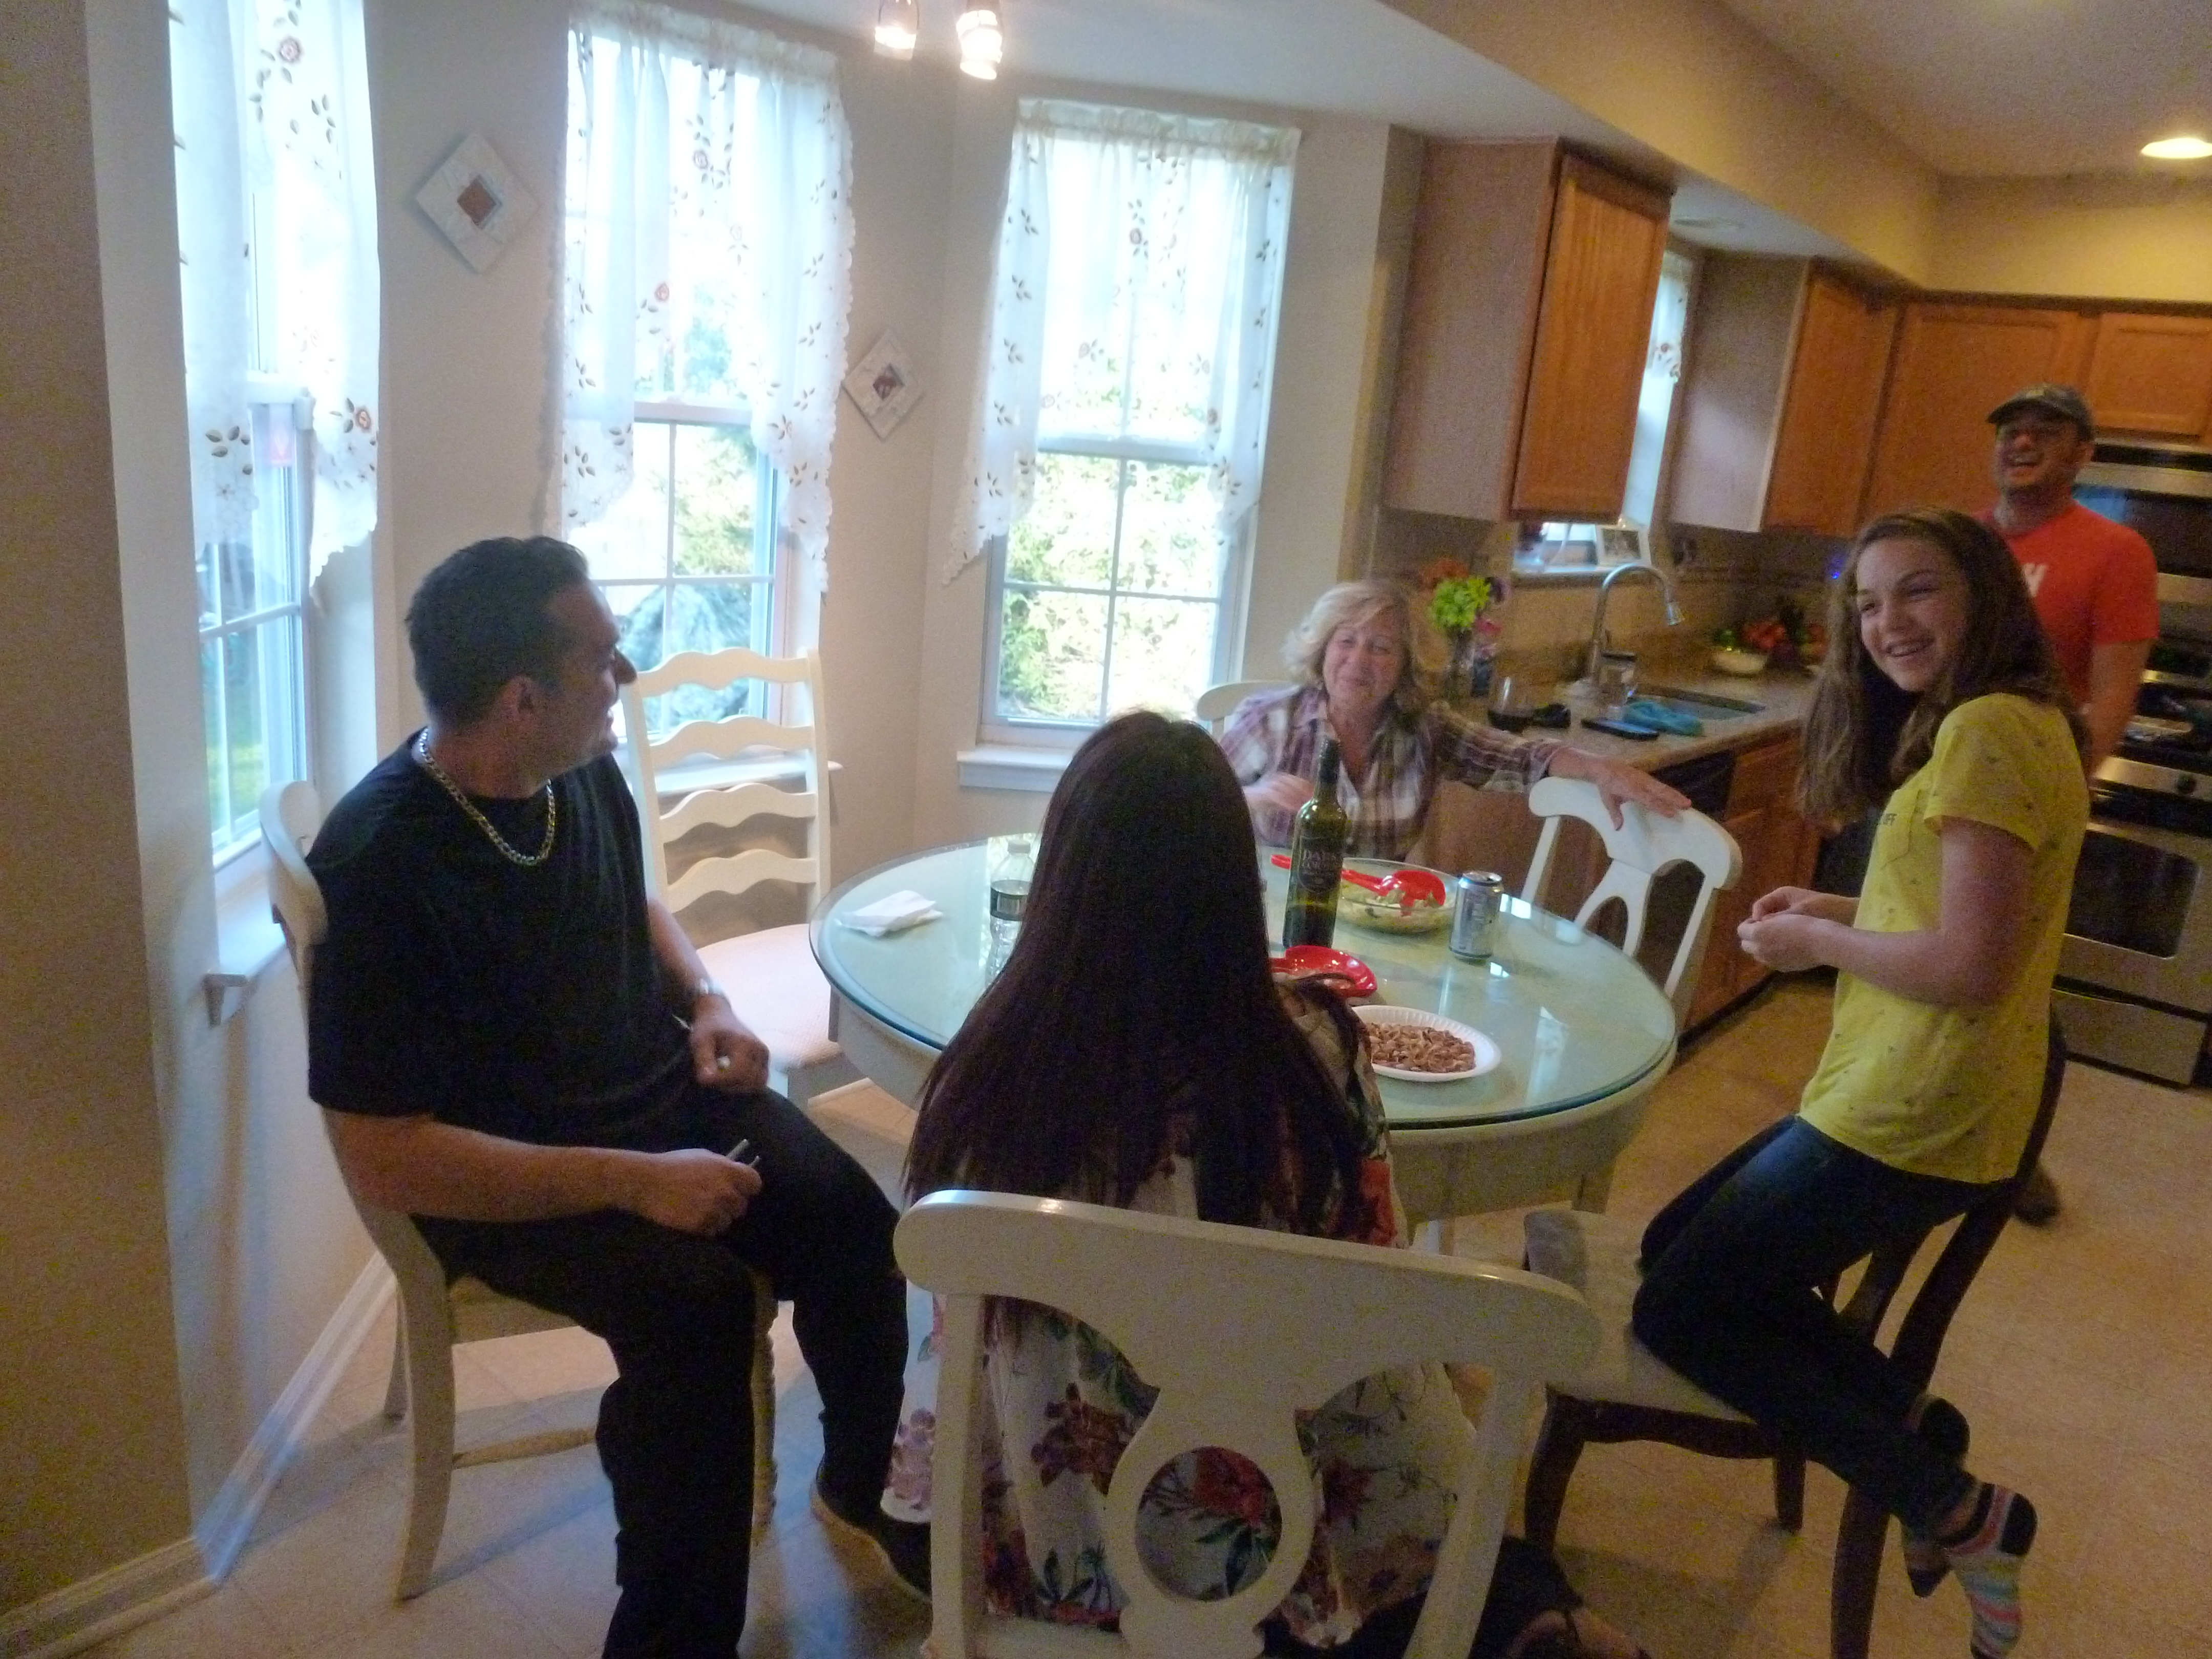
\includegraphics[width=0.6\linewidth,height=\textheight,keepaspectratio]{chapters/../images/P1020477.JPG}

}

\caption{The family, September 2017}

\end{figure}%

\begin{figure}[H]

{\centering \includegraphics[width=0.35\linewidth,height=\textheight,keepaspectratio]{chapters/../images/recent/cicc.jpg}

}

\caption{Vic}

\end{figure}%

\begin{center}\rule{0.5\linewidth}{0.5pt}\end{center}

Happy 80th birthday, Dad.

\emph{The best is yet to come.}

\begin{center}\rule{0.5\linewidth}{0.5pt}\end{center}

{Love, Your Family}

\begin{center}\rule{0.5\linewidth}{0.5pt}\end{center}

\emph{Prepared with love by the Cicconetti family, March 2026.}

\cleardoublepage
\phantomsection
\addcontentsline{toc}{part}{Appendices}
\appendix

\chapter*{Life Timeline}\label{timeline}
\addcontentsline{toc}{chapter}{Life Timeline}

\markboth{Life Timeline}{Life Timeline}

\section*{Victor R. Cicconetti --- Eighty
Years}\label{victor-r.-cicconetti-eighty-years}
\addcontentsline{toc}{section}{Victor R. Cicconetti --- Eighty Years}

\markright{Victor R. Cicconetti --- Eighty Years}

\phantomsection\label{timeline-table}
\begin{longtable}[]{@{}
  >{\raggedright\arraybackslash}p{(\linewidth - 8\tabcolsep) * \real{0.1500}}
  >{\raggedright\arraybackslash}p{(\linewidth - 8\tabcolsep) * \real{0.1750}}
  >{\centering\arraybackslash}p{(\linewidth - 8\tabcolsep) * \real{0.1500}}
  >{\centering\arraybackslash}p{(\linewidth - 8\tabcolsep) * \real{0.1750}}
  >{\centering\arraybackslash}p{(\linewidth - 8\tabcolsep) * \real{0.3500}}@{}}
\caption{Victor R. Cicconetti --- Life Timeline}\tabularnewline
\toprule\noalign{}
\begin{minipage}[b]{\linewidth}\raggedright
Year
\end{minipage} & \begin{minipage}[b]{\linewidth}\raggedright
Event
\end{minipage} & \begin{minipage}[b]{\linewidth}\centering
TRUE
\end{minipage} & \begin{minipage}[b]{\linewidth}\centering
FALSE
\end{minipage} & \begin{minipage}[b]{\linewidth}\centering
I DON'T KNOW
\end{minipage} \\
\midrule\noalign{}
\endfirsthead
\toprule\noalign{}
\begin{minipage}[b]{\linewidth}\raggedright
Year
\end{minipage} & \begin{minipage}[b]{\linewidth}\raggedright
Event
\end{minipage} & \begin{minipage}[b]{\linewidth}\centering
TRUE
\end{minipage} & \begin{minipage}[b]{\linewidth}\centering
FALSE
\end{minipage} & \begin{minipage}[b]{\linewidth}\centering
I DON'T KNOW
\end{minipage} \\
\midrule\noalign{}
\endhead
\bottomrule\noalign{}
\endlastfoot
\textasciitilde1946 & Born in New York City (10th St \& Ave C); family
moves to Bayonne \textasciitilde age 10 & & & \\
1964 & Joins U.S. Air Force --- basic training at Lackland AFB, TX & &
& \\
1966--1967 & Stationed at Shreveport, LA & & & \\
1967 & Marries Yvonne C. Elia, August 20, Assumption Church, Bayonne & &
& \\
1968 & Deployed to Thailand --- medical air evacuations in Southeast
Asia & & & \\
1969 & Completes Air Force service; honorable discharge; first married
home at 84 Humphrey's Ave, Bayonne & & & \\
1971 & Brief move to San Diego, CA; returns to Bayonne & & & \\
1974--1977 & Family at 158 W 21st St, Bayonne & & & \\
1977 & Son Richard ``Rich'' born (\textasciitilde August); buy first
home on Avenue E, Bayonne & & & \\
1980 & Father Victor Sr.~passes away (age \textasciitilde55); family
moves to 104 Highland Ave, Shark River Hills & & & \\
1980--1995 & Administrator at Long Branch High School; living in Shark
River Hills & & & \\
1987 & Featured in \emph{Red Bank Register} --- ``Man with Many
Missions'' & & & \\
1995 & Moves to 4 Rue de la Porte, Wall, NJ & & & \\
1990s & Administrator in Asbury Park school district & & & \\
1997 & Mother Eleanor passes away & & & \\
2000 & Retires from public school administration; moves to 18 Waterview
Ave, Neptune & & & \\
2005 & Yvonne retires from Jersey City public schools & & & \\
2007 & 40th wedding anniversary (4 grandchildren at that time) & & & \\
2009 & Brother Michael C. Cicconetti passes away & & & \\
2020 & Moves to 671 Cypress Pt Dr, Blue Heron Pines (Egg Harbor City) &
& & \\
\textasciitilde2025 & Sister Loretta Keating passes away & & & \\
2026 & Turns 80 --- \textbf{this celebration} & & & \\
\end{longtable}

\begin{tcolorbox}[enhanced jigsaw, left=2mm, leftrule=.75mm, opacityback=0, breakable, colframe=quarto-callout-note-color-frame, toprule=.15mm, bottomrule=.15mm, colback=white, arc=.35mm, rightrule=.15mm]
\begin{minipage}[t]{5.5mm}
\textcolor{quarto-callout-note-color}{\faInfo}
\end{minipage}%
\begin{minipage}[t]{\textwidth - 5.5mm}

\textbf{Check our work --- Timeline:}

\emph{(Any dates wrong? Any approximate dates you know exactly? Any
major life events we missed entirely?)}

\hfill\break

\end{minipage}%
\end{tcolorbox}

\subsection*{Undated Events}\label{undated-events}
\addcontentsline{toc}{subsection}{Undated Events}

The following milestones are confirmed but we don't know when they
happened. Can you fill in the years?

\begin{longtable}[]{@{}
  >{\raggedright\arraybackslash}p{(\linewidth - 8\tabcolsep) * \real{0.1707}}
  >{\centering\arraybackslash}p{(\linewidth - 8\tabcolsep) * \real{0.1707}}
  >{\centering\arraybackslash}p{(\linewidth - 8\tabcolsep) * \real{0.1463}}
  >{\centering\arraybackslash}p{(\linewidth - 8\tabcolsep) * \real{0.1707}}
  >{\centering\arraybackslash}p{(\linewidth - 8\tabcolsep) * \real{0.3415}}@{}}
\toprule\noalign{}
\begin{minipage}[b]{\linewidth}\raggedright
Event
\end{minipage} & \begin{minipage}[b]{\linewidth}\centering
Year?
\end{minipage} & \begin{minipage}[b]{\linewidth}\centering
TRUE
\end{minipage} & \begin{minipage}[b]{\linewidth}\centering
FALSE
\end{minipage} & \begin{minipage}[b]{\linewidth}\centering
I DON'T KNOW
\end{minipage} \\
\midrule\noalign{}
\endhead
\bottomrule\noalign{}
\endlastfoot
Victor, Yvonne, and Richard co-found Bistro-by-the-Sea in
Avon-by-the-Sea, NJ & & & & \\
Victor founds VVA Chapter 12 in Ocean Township, NJ; serves as president
& & & & \\
Victor becomes life member of VA and DAV & & & & \\
Rich Cicconetti marries Sharon K. Doughty & & & & \\
5th and 6th grandchildren born (after 2007) & & & & \\
\end{longtable}

\begin{tcolorbox}[enhanced jigsaw, toptitle=1mm, opacitybacktitle=0.6, leftrule=.75mm, breakable, toprule=.15mm, colbacktitle=quarto-callout-tip-color!10!white, titlerule=0mm, left=2mm, opacityback=0, colframe=quarto-callout-tip-color-frame, bottomtitle=1mm, title=\textcolor{quarto-callout-tip-color}{\faLightbulb}\hspace{0.5em}{Tell Us a Story}, arc=.35mm, colback=white, coltitle=black, rightrule=.15mm, bottomrule=.15mm]

\textbf{Everyone:} Look at this timeline. What's the biggest thing
missing? The event that should be on this list but isn't? Don't think
about it too hard --- just name the first thing that comes to mind.

\textbf{Dad:} What year would you say was the best year of your life?
And what year was the hardest?

\end{tcolorbox}

\chapter*{Life Journey Map}\label{life-map}
\addcontentsline{toc}{chapter}{Life Journey Map}

\markboth{Life Journey Map}{Life Journey Map}

From a Manhattan tenement to the Jersey Shore to a golf community in the
Pines --- eighty years of addresses, on one map.

\emph{The interactive Life Journey Map is available in the online
version of this book. It traces Victor's 21 addresses from 10th St \&
Avenue C in Manhattan (1946) through 671 Cypress Point Drive at Blue
Heron Pines (2020--present), with animated fly-through and era-colored
markers.}

\begin{tcolorbox}[enhanced jigsaw, toptitle=1mm, opacitybacktitle=0.6, leftrule=.75mm, breakable, toprule=.15mm, colbacktitle=quarto-callout-tip-color!10!white, titlerule=0mm, left=2mm, opacityback=0, colframe=quarto-callout-tip-color-frame, bottomtitle=1mm, title=\textcolor{quarto-callout-tip-color}{\faLightbulb}\hspace{0.5em}{Help Us Fill In the Gaps}, arc=.35mm, colback=white, coltitle=black, rightrule=.15mm, bottomrule=.15mm]

\textbf{Dad \& Mom:} We have the addresses but not always the stories.
Pick any pin on the map and tell us what you remember about living
there. What did the house look like? Who were the neighbors? What was
happening in your life at that address?

\textbf{Anyone:} Do you remember visiting Vic and Yvonne at any of these
addresses? What's the memory?

\end{tcolorbox}

\chapter*{Family Tree}\label{family-tree}
\addcontentsline{toc}{chapter}{Family Tree}

\markboth{Family Tree}{Family Tree}

The Cicconetti family spans four generations --- from Victor Sr.~and
Eleanor in Bayonne to three grandchildren carrying the legacy forward
today.

\section*{Generation 1: The Parents}\label{generation-1-the-parents}
\addcontentsline{toc}{section}{Generation 1: The Parents}

\markright{Generation 1: The Parents}

\begin{verbatim}
Victor Cicconetti Sr. (1925–1980)  ─── m. ───  Eleanor Salone (d. 1997)
                                                  │
Frank Elia (d. ~1962)  ─── m. ───  Mary Chiarolanza (b. ~1920, Italy)
\end{verbatim}

\section*{Generation 2: Victor's Siblings \&
Yvonne}\label{generation-2-victors-siblings-yvonne}
\addcontentsline{toc}{section}{Generation 2: Victor's Siblings \&
Yvonne}

\markright{Generation 2: Victor's Siblings \& Yvonne}

\begin{longtable}[]{@{}
  >{\raggedright\arraybackslash}p{(\linewidth - 6\tabcolsep) * \real{0.2069}}
  >{\raggedright\arraybackslash}p{(\linewidth - 6\tabcolsep) * \real{0.2759}}
  >{\raggedright\arraybackslash}p{(\linewidth - 6\tabcolsep) * \real{0.2759}}
  >{\raggedright\arraybackslash}p{(\linewidth - 6\tabcolsep) * \real{0.2414}}@{}}
\caption{Generation 2 --- The Cicconetti Six and the Elia
Sisters}\tabularnewline
\toprule\noalign{}
\begin{minipage}[b]{\linewidth}\raggedright
Name
\end{minipage} & \begin{minipage}[b]{\linewidth}\raggedright
Status
\end{minipage} & \begin{minipage}[b]{\linewidth}\raggedright
Spouse
\end{minipage} & \begin{minipage}[b]{\linewidth}\raggedright
Notes
\end{minipage} \\
\midrule\noalign{}
\endfirsthead
\toprule\noalign{}
\begin{minipage}[b]{\linewidth}\raggedright
Name
\end{minipage} & \begin{minipage}[b]{\linewidth}\raggedright
Status
\end{minipage} & \begin{minipage}[b]{\linewidth}\raggedright
Spouse
\end{minipage} & \begin{minipage}[b]{\linewidth}\raggedright
Notes
\end{minipage} \\
\midrule\noalign{}
\endhead
\bottomrule\noalign{}
\endlastfoot
\textbf{Victor R. Cicconetti} & Living (b. March 29, 1946) & Yvonne (nee
Elia) & The birthday honoree --- ``Grandpa'' \\
Dennis Cicconetti & Deceased (pre-2009) & --- & Brother \\
Rev.~Leanora Cicconetti & Living (\textasciitilde67) & Clavelli &
Sister; reverend; genealogist \\
Robert ``Bob'' Cicconetti & Living & Ret. Lt. Col. Elizabeth &
Brother \\
Loretta Keating & Deceased (\textasciitilde2025) & Louis Keating &
Sister \\
Michael C. Cicconetti & Deceased (2009) & Karen Haraksin & Brother; son
Christopher \\
Mary Ann Hurley & Living & Michael Hurley Sr.~(Ret. Capt., Bayonne PD) &
Yvonne's sister \\
\end{longtable}

\section*{Generation 3: Victor \& Yvonne's
Children}\label{generation-3-victor-yvonnes-children}
\addcontentsline{toc}{section}{Generation 3: Victor \& Yvonne's
Children}

\markright{Generation 3: Victor \& Yvonne's Children}

\begin{longtable}[]{@{}
  >{\raggedright\arraybackslash}p{(\linewidth - 6\tabcolsep) * \real{0.2222}}
  >{\raggedright\arraybackslash}p{(\linewidth - 6\tabcolsep) * \real{0.2222}}
  >{\raggedright\arraybackslash}p{(\linewidth - 6\tabcolsep) * \real{0.2963}}
  >{\raggedright\arraybackslash}p{(\linewidth - 6\tabcolsep) * \real{0.2593}}@{}}
\caption{Generation 3 --- Victor and Yvonne's Two Sons}\tabularnewline
\toprule\noalign{}
\begin{minipage}[b]{\linewidth}\raggedright
Name
\end{minipage} & \begin{minipage}[b]{\linewidth}\raggedright
Born
\end{minipage} & \begin{minipage}[b]{\linewidth}\raggedright
Spouse
\end{minipage} & \begin{minipage}[b]{\linewidth}\raggedright
Notes
\end{minipage} \\
\midrule\noalign{}
\endfirsthead
\toprule\noalign{}
\begin{minipage}[b]{\linewidth}\raggedright
Name
\end{minipage} & \begin{minipage}[b]{\linewidth}\raggedright
Born
\end{minipage} & \begin{minipage}[b]{\linewidth}\raggedright
Spouse
\end{minipage} & \begin{minipage}[b]{\linewidth}\raggedright
Notes
\end{minipage} \\
\midrule\noalign{}
\endhead
\bottomrule\noalign{}
\endlastfoot
\textbf{Greg Cicconetti} & --- & 1st: Jennifer Feulmer (b. May 23,
1976); 2nd: Valerie (div. 2025) & Ph.D., Research Fellow (AbbVie);
father of Ellie and Anthony (with Jennifer) \\
\textbf{Richard Victor Cicconetti} & \textasciitilde1977 & Sharon K.
Doughty & Rutgers; Cicco Devel; co-founded Bistro-by-the-Sea; father of
Richy \\
\end{longtable}

\section*{Generation 4: The
Grandchildren}\label{generation-4-the-grandchildren}
\addcontentsline{toc}{section}{Generation 4: The Grandchildren}

\markright{Generation 4: The Grandchildren}

Victor and Yvonne have \textbf{three biological grandchildren}:

\begin{longtable}[]{@{}
  >{\raggedright\arraybackslash}p{(\linewidth - 4\tabcolsep) * \real{0.2857}}
  >{\raggedright\arraybackslash}p{(\linewidth - 4\tabcolsep) * \real{0.3810}}
  >{\raggedright\arraybackslash}p{(\linewidth - 4\tabcolsep) * \real{0.3333}}@{}}
\caption{Generation 4 --- The Grandchildren}\tabularnewline
\toprule\noalign{}
\begin{minipage}[b]{\linewidth}\raggedright
Name
\end{minipage} & \begin{minipage}[b]{\linewidth}\raggedright
Parent
\end{minipage} & \begin{minipage}[b]{\linewidth}\raggedright
Notes
\end{minipage} \\
\midrule\noalign{}
\endfirsthead
\toprule\noalign{}
\begin{minipage}[b]{\linewidth}\raggedright
Name
\end{minipage} & \begin{minipage}[b]{\linewidth}\raggedright
Parent
\end{minipage} & \begin{minipage}[b]{\linewidth}\raggedright
Notes
\end{minipage} \\
\midrule\noalign{}
\endhead
\bottomrule\noalign{}
\endlastfoot
\textbf{Ellie Wexler} & Greg \& Jennifer & b. October 22, 2003; also
known as Natalie Cicconetti / Ellie Cicconetti \\
\textbf{Anthony John Cicconetti} & Greg \& Jennifer & b. July 25,
2008 \\
\textbf{Richard Victor Cicconetti Jr.~(``Richy'')} & Rich \& Sharon & \\
\end{longtable}

Vic also embraced \textbf{Hunter} and \textbf{Noah} --- twin sons of
Greg's second wife Valerie from her first marriage --- as his own
grandchildren. At the 75th birthday in 2021, all five were part of the
celebration.

\section*{Legend}\label{legend}
\addcontentsline{toc}{section}{Legend}

\markright{Legend}

\begin{longtable}[]{@{}ll@{}}
\toprule\noalign{}
Color / Style & Meaning \\
\midrule\noalign{}
\endhead
\bottomrule\noalign{}
\endlastfoot
\textbf{Bold} & Living \\
\emph{Italic} & Placeholder --- name not yet confirmed \\
Struck or noted ``Deceased'' & Deceased \\
\end{longtable}

\section*{Visual Family Tree}\label{visual-family-tree}
\addcontentsline{toc}{section}{Visual Family Tree}

\markright{Visual Family Tree}

\begin{figure}[H]

{\centering \includegraphics[width=1\linewidth,height=\textheight,keepaspectratio]{appendices/../images/family/family_tree.png}

}

\caption{The Cicconetti Family Tree --- dashed borders indicate names we
still need.}

\end{figure}%

\textbf{Family tree updated with corrections from Anthony Cicconetti,
February 2026.} See \texttt{data/family.json} for the current data
structure.

\chapter*{Correct the Record}\label{correct-the-record}
\addcontentsline{toc}{chapter}{Correct the Record}

\markboth{Correct the Record}{Correct the Record}

\emph{Dad, Mom --- we did our homework. We dug through newspapers,
public records, census data, and old emails. We're pretty sure we got
most of it right. But this is YOUR story, not ours. So here's everything
we think we know. Tell us where we nailed it, where we blew it, and what
we missed entirely.}

\section*{How This Works}\label{how-this-works}
\addcontentsline{toc}{section}{How This Works}

\markright{How This Works}

We've listed every factual claim in this book. For each one, just pick
one:

\begin{longtable}[]{@{}ll@{}}
\toprule\noalign{}
& Meaning \\
\midrule\noalign{}
\endhead
\bottomrule\noalign{}
\endlastfoot
\textbf{TRUE} & Yes, that's right \\
\textbf{FALSE} & No, that's wrong \\
\textbf{I DON'T KNOW} & Not sure / don't remember \\
\end{longtable}

After each section, there's a space to set the record straight ---
correct what we got wrong, fill in what we missed, or just tell us more.

\begin{tcolorbox}[enhanced jigsaw, toptitle=1mm, opacitybacktitle=0.6, leftrule=.75mm, breakable, toprule=.15mm, colbacktitle=quarto-callout-important-color!10!white, titlerule=0mm, left=2mm, opacityback=0, colframe=quarto-callout-important-color-frame, bottomtitle=1mm, title=\textcolor{quarto-callout-important-color}{\faExclamation}\hspace{0.5em}{Respond Online}, arc=.35mm, colback=white, coltitle=black, rightrule=.15mm, bottomrule=.15mm]

\textbf{Prefer to fill this out on your phone or computer?} Use the
online form --- it takes about 10 minutes and your answers go straight
to Greg.

\href{https://docs.google.com/forms/d/e/1FAIpQLSewx8qzirtlXs1__lK0o1AXk9k54Ib-6nhrPtm3Ul5sFrY2Vw/viewform}{Open
the Fact-Check Form}

\end{tcolorbox}

\begin{center}\rule{0.5\linewidth}{0.5pt}\end{center}

\section*{Chapter 1: Two Families, One
City}\label{chapter-1-two-families-one-city}
\addcontentsline{toc}{section}{Chapter 1: Two Families, One City}

\markright{Chapter 1: Two Families, One City}

\subsection*{The Cicconetti Side}\label{the-cicconetti-side}
\addcontentsline{toc}{subsection}{The Cicconetti Side}

\begin{longtable}[]{@{}
  >{\raggedright\arraybackslash}p{(\linewidth - 8\tabcolsep) * \real{0.0732}}
  >{\raggedright\arraybackslash}p{(\linewidth - 8\tabcolsep) * \real{0.2683}}
  >{\centering\arraybackslash}p{(\linewidth - 8\tabcolsep) * \real{0.1463}}
  >{\centering\arraybackslash}p{(\linewidth - 8\tabcolsep) * \real{0.1707}}
  >{\centering\arraybackslash}p{(\linewidth - 8\tabcolsep) * \real{0.3415}}@{}}
\toprule\noalign{}
\begin{minipage}[b]{\linewidth}\raggedright
\#
\end{minipage} & \begin{minipage}[b]{\linewidth}\raggedright
We wrote\ldots{}
\end{minipage} & \begin{minipage}[b]{\linewidth}\centering
TRUE
\end{minipage} & \begin{minipage}[b]{\linewidth}\centering
FALSE
\end{minipage} & \begin{minipage}[b]{\linewidth}\centering
I DON'T KNOW
\end{minipage} \\
\midrule\noalign{}
\endhead
\bottomrule\noalign{}
\endlastfoot
1 & The Cicconetti name traces to Collepietro, Abruzzo, Italy & & & \\
2 & The name means ``little Cicco,'' from Franciscus & & & \\
3 & The family has been in Collepietro since at least 1778 & & & \\
4 & Victor Sr.~was born in Bayonne in 1925 & & & \\
5 & Victor Sr.~married Eleanor Salone & & & \\
6 & Eleanor was one of three Salone sisters: Marge, Eleanor, Josie & &
& \\
7 & The Salone sisters grew up on the Lower East Side of Manhattan & &
& \\
8 & During the Depression, the sisters spent time in an orphanage & &
& \\
9 & Their mother Anna worked as a sweatshop seamstress & & & \\
10 & Victor Sr.~and Eleanor raised six children in Bayonne & & & \\
11 & The six children were: Victor, Dennis, Leanora, Bob, Loretta,
Michael & & & \\
12 & Victor Sr.~died in 1980 & & & \\
13 & Eleanor died in 1997 & & & \\
\end{longtable}

\begin{tcolorbox}[enhanced jigsaw, left=2mm, leftrule=.75mm, opacityback=0, breakable, colframe=quarto-callout-note-color-frame, toprule=.15mm, bottomrule=.15mm, colback=white, arc=.35mm, rightrule=.15mm]
\begin{minipage}[t]{5.5mm}
\textcolor{quarto-callout-note-color}{\faInfo}
\end{minipage}%
\begin{minipage}[t]{\textwidth - 5.5mm}

\textbf{Set the record straight --- The Cicconetti Side:}

\emph{(What did we get wrong? What did we miss? Tell us anything about
the Cicconetti family history.)}

\hfill\break

\end{minipage}%
\end{tcolorbox}

\subsection*{The Elia / Chiarolanza
Side}\label{the-elia-chiarolanza-side}
\addcontentsline{toc}{subsection}{The Elia / Chiarolanza Side}

\begin{longtable}[]{@{}
  >{\raggedright\arraybackslash}p{(\linewidth - 8\tabcolsep) * \real{0.0732}}
  >{\raggedright\arraybackslash}p{(\linewidth - 8\tabcolsep) * \real{0.2683}}
  >{\centering\arraybackslash}p{(\linewidth - 8\tabcolsep) * \real{0.1463}}
  >{\centering\arraybackslash}p{(\linewidth - 8\tabcolsep) * \real{0.1707}}
  >{\centering\arraybackslash}p{(\linewidth - 8\tabcolsep) * \real{0.3415}}@{}}
\toprule\noalign{}
\begin{minipage}[b]{\linewidth}\raggedright
\#
\end{minipage} & \begin{minipage}[b]{\linewidth}\raggedright
We wrote\ldots{}
\end{minipage} & \begin{minipage}[b]{\linewidth}\centering
TRUE
\end{minipage} & \begin{minipage}[b]{\linewidth}\centering
FALSE
\end{minipage} & \begin{minipage}[b]{\linewidth}\centering
I DON'T KNOW
\end{minipage} \\
\midrule\noalign{}
\endhead
\bottomrule\noalign{}
\endlastfoot
14 & Yvonne's mother Mary's maiden name was Chiarolanza (family
spelling: Chirolanza) & & & \\
15 & The Chiarolanza family came from Campania, likely Montecorvino
Rovella & & & \\
16 & The 1940 Census shows Mary (age 20) in Bayonne with father Alfonso,
mother Angelina, and 4 sisters & & & \\
17 & Mary worked as a seamstress at the Maidenform factory, 154 Avenue E
& & & \\
18 & Frank Elia worked as a poultry processor & & & \\
19 & Frank died around 1962, when Yvonne was about 14 & & & \\
20 & After Frank's death, Mary married Anthony Galella & & & \\
21 & Greg named his son Anthony after Anthony Galella & & & \\
\end{longtable}

\begin{tcolorbox}[enhanced jigsaw, left=2mm, leftrule=.75mm, opacityback=0, breakable, colframe=quarto-callout-note-color-frame, toprule=.15mm, bottomrule=.15mm, colback=white, arc=.35mm, rightrule=.15mm]
\begin{minipage}[t]{5.5mm}
\textcolor{quarto-callout-note-color}{\faInfo}
\end{minipage}%
\begin{minipage}[t]{\textwidth - 5.5mm}

\textbf{Set the record straight --- The Elia / Chiarolanza Side:}

\emph{(What did we get wrong? What did we miss? Tell us anything about
Mom's family.)}

\hfill\break

\end{minipage}%
\end{tcolorbox}

\begin{center}\rule{0.5\linewidth}{0.5pt}\end{center}

\section*{Chapter 2: Two Paths}\label{chapter-2-two-paths}
\addcontentsline{toc}{section}{Chapter 2: Two Paths}

\markright{Chapter 2: Two Paths}

\subsection*{Victor's Military Service}\label{victors-military-service}
\addcontentsline{toc}{subsection}{Victor's Military Service}

\begin{longtable}[]{@{}llccc@{}}
\toprule\noalign{}
\# & We wrote\ldots{} & TRUE & FALSE & I DON'T KNOW \\
\midrule\noalign{}
\endhead
\bottomrule\noalign{}
\endlastfoot
22 & Victor joined the Air Force in 1965 at age 19 & & & \\
23 & He served as a medic & & & \\
24 & He flew medical air evacuations in Southeast Asia & & & \\
25 & His service ended in 1969 & & & \\
26 & ``MedFlyBoy'' was his nickname from service & & & \\
\end{longtable}

\begin{tcolorbox}[enhanced jigsaw, left=2mm, leftrule=.75mm, opacityback=0, breakable, colframe=quarto-callout-note-color-frame, toprule=.15mm, bottomrule=.15mm, colback=white, arc=.35mm, rightrule=.15mm]
\begin{minipage}[t]{5.5mm}
\textcolor{quarto-callout-note-color}{\faInfo}
\end{minipage}%
\begin{minipage}[t]{\textwidth - 5.5mm}

\textbf{Set the record straight --- Victor's Military Service:}

\emph{(Bases, units, buddies, stories --- anything you can tell us about
those years.)}

\hfill\break

\end{minipage}%
\end{tcolorbox}

\subsection*{Yvonne's Early Life}\label{yvonnes-early-life}
\addcontentsline{toc}{subsection}{Yvonne's Early Life}

\begin{longtable}[]{@{}llccc@{}}
\toprule\noalign{}
\# & We wrote\ldots{} & TRUE & FALSE & I DON'T KNOW \\
\midrule\noalign{}
\endhead
\bottomrule\noalign{}
\endlastfoot
27 & Yvonne was born approximately April 1948 & & & \\
28 & She grew up in Bayonne & & & \\
29 & Losing her father at \textasciitilde14 shaped her resilience & &
& \\
30 & Her sister Mary Ann was her closest bond & & & \\
\end{longtable}

\begin{tcolorbox}[enhanced jigsaw, left=2mm, leftrule=.75mm, opacityback=0, breakable, colframe=quarto-callout-note-color-frame, toprule=.15mm, bottomrule=.15mm, colback=white, arc=.35mm, rightrule=.15mm]
\begin{minipage}[t]{5.5mm}
\textcolor{quarto-callout-note-color}{\faInfo}
\end{minipage}%
\begin{minipage}[t]{\textwidth - 5.5mm}

\textbf{Set the record straight --- Yvonne's Early Life:}

\emph{(Mom, what do you remember about growing up? Where did you go to
school? What were you like as a kid?)}

\hfill\break

\end{minipage}%
\end{tcolorbox}

\begin{center}\rule{0.5\linewidth}{0.5pt}\end{center}

\section*{Chapter 3: August 20, 1967}\label{chapter-3-august-20-1967}
\addcontentsline{toc}{section}{Chapter 3: August 20, 1967}

\markright{Chapter 3: August 20, 1967}

\begin{longtable}[]{@{}llccc@{}}
\toprule\noalign{}
\# & We wrote\ldots{} & TRUE & FALSE & I DON'T KNOW \\
\midrule\noalign{}
\endhead
\bottomrule\noalign{}
\endlastfoot
31 & Victor and Yvonne married on August 20, 1967 & & & \\
32 & The wedding was at Assumption Catholic Church, Bayonne & & & \\
33 & Victor was 21, Yvonne was 19 & & & \\
34 & Victor was still in the Air Force when they married & & & \\
\end{longtable}

\begin{tcolorbox}[enhanced jigsaw, left=2mm, leftrule=.75mm, opacityback=0, breakable, colframe=quarto-callout-note-color-frame, toprule=.15mm, bottomrule=.15mm, colback=white, arc=.35mm, rightrule=.15mm]
\begin{minipage}[t]{5.5mm}
\textcolor{quarto-callout-note-color}{\faInfo}
\end{minipage}%
\begin{minipage}[t]{\textwidth - 5.5mm}

\textbf{Set the record straight --- The Wedding:}

\emph{(How did you two meet? Who introduced you? What do you remember
about the wedding day?)}

\hfill\break

\end{minipage}%
\end{tcolorbox}

\begin{center}\rule{0.5\linewidth}{0.5pt}\end{center}

\section*{Chapter 4: Man with Many
Missions}\label{chapter-4-man-with-many-missions}
\addcontentsline{toc}{section}{Chapter 4: Man with Many Missions}

\markright{Chapter 4: Man with Many Missions}

\begin{longtable}[]{@{}
  >{\raggedright\arraybackslash}p{(\linewidth - 8\tabcolsep) * \real{0.0732}}
  >{\raggedright\arraybackslash}p{(\linewidth - 8\tabcolsep) * \real{0.2683}}
  >{\centering\arraybackslash}p{(\linewidth - 8\tabcolsep) * \real{0.1463}}
  >{\centering\arraybackslash}p{(\linewidth - 8\tabcolsep) * \real{0.1707}}
  >{\centering\arraybackslash}p{(\linewidth - 8\tabcolsep) * \real{0.3415}}@{}}
\toprule\noalign{}
\begin{minipage}[b]{\linewidth}\raggedright
\#
\end{minipage} & \begin{minipage}[b]{\linewidth}\raggedright
We wrote\ldots{}
\end{minipage} & \begin{minipage}[b]{\linewidth}\centering
TRUE
\end{minipage} & \begin{minipage}[b]{\linewidth}\centering
FALSE
\end{minipage} & \begin{minipage}[b]{\linewidth}\centering
I DON'T KNOW
\end{minipage} \\
\midrule\noalign{}
\endhead
\bottomrule\noalign{}
\endlastfoot
35 & Victor was an administrator at Long Branch High School in the 1980s
& & & \\
36 & The Red Bank Register profiled him in 1987 as ``Man with Many
Missions'' & & & \\
37 & He also worked in the Asbury Park school district & & & \\
38 & He retired from education in 2000 & & & \\
39 & Yvonne taught health in Jersey City public schools & & & \\
40 & Yvonne retired in 2005 & & & \\
41 & Yvonne then served as Allied Health Vocational advisor for Hudson
County & & & \\
\end{longtable}

\begin{tcolorbox}[enhanced jigsaw, left=2mm, leftrule=.75mm, opacityback=0, breakable, colframe=quarto-callout-note-color-frame, toprule=.15mm, bottomrule=.15mm, colback=white, arc=.35mm, rightrule=.15mm]
\begin{minipage}[t]{5.5mm}
\textcolor{quarto-callout-note-color}{\faInfo}
\end{minipage}%
\begin{minipage}[t]{\textwidth - 5.5mm}

\textbf{Set the record straight --- Careers:}

\emph{(What were the schools like? Favorite students? Best stories from
the classroom? The ``Man with Many Missions'' article --- do you still
have a copy?)}

\hfill\break

\end{minipage}%
\end{tcolorbox}

\begin{center}\rule{0.5\linewidth}{0.5pt}\end{center}

\section*{Chapter 5: The Family Table}\label{chapter-5-the-family-table}
\addcontentsline{toc}{section}{Chapter 5: The Family Table}

\markright{Chapter 5: The Family Table}

\begin{longtable}[]{@{}
  >{\raggedright\arraybackslash}p{(\linewidth - 8\tabcolsep) * \real{0.0732}}
  >{\raggedright\arraybackslash}p{(\linewidth - 8\tabcolsep) * \real{0.2683}}
  >{\centering\arraybackslash}p{(\linewidth - 8\tabcolsep) * \real{0.1463}}
  >{\centering\arraybackslash}p{(\linewidth - 8\tabcolsep) * \real{0.1707}}
  >{\centering\arraybackslash}p{(\linewidth - 8\tabcolsep) * \real{0.3415}}@{}}
\toprule\noalign{}
\begin{minipage}[b]{\linewidth}\raggedright
\#
\end{minipage} & \begin{minipage}[b]{\linewidth}\raggedright
We wrote\ldots{}
\end{minipage} & \begin{minipage}[b]{\linewidth}\centering
TRUE
\end{minipage} & \begin{minipage}[b]{\linewidth}\centering
FALSE
\end{minipage} & \begin{minipage}[b]{\linewidth}\centering
I DON'T KNOW
\end{minipage} \\
\midrule\noalign{}
\endhead
\bottomrule\noalign{}
\endlastfoot
42 & Victor, Yvonne, and Richard co-founded Bistro-by-the-Sea in
Avon-by-the-Sea, NJ & & & \\
43 & Mary Ann Hurley ran a pizza bistro in Bayonne & & & \\
\end{longtable}

\begin{tcolorbox}[enhanced jigsaw, left=2mm, leftrule=.75mm, opacityback=0, breakable, colframe=quarto-callout-warning-color-frame, toprule=.15mm, bottomrule=.15mm, colback=white, arc=.35mm, rightrule=.15mm]
\begin{minipage}[t]{5.5mm}
\textcolor{quarto-callout-warning-color}{\faExclamationTriangle}
\end{minipage}%
\begin{minipage}[t]{\textwidth - 5.5mm}

\textbf{This section is almost empty without you!}

\emph{(What was the restaurant called? Where was it? What years? Which
son? What were the signature dishes? What was it like running a
restaurant as a family? How about Mary Ann's pizza bistro?)}

\hfill\break

\end{minipage}%
\end{tcolorbox}

\begin{center}\rule{0.5\linewidth}{0.5pt}\end{center}

\section*{Chapter 6: Serving Those Who
Served}\label{chapter-6-serving-those-who-served}
\addcontentsline{toc}{section}{Chapter 6: Serving Those Who Served}

\markright{Chapter 6: Serving Those Who Served}

\begin{longtable}[]{@{}
  >{\raggedright\arraybackslash}p{(\linewidth - 8\tabcolsep) * \real{0.0732}}
  >{\raggedright\arraybackslash}p{(\linewidth - 8\tabcolsep) * \real{0.2683}}
  >{\centering\arraybackslash}p{(\linewidth - 8\tabcolsep) * \real{0.1463}}
  >{\centering\arraybackslash}p{(\linewidth - 8\tabcolsep) * \real{0.1707}}
  >{\centering\arraybackslash}p{(\linewidth - 8\tabcolsep) * \real{0.3415}}@{}}
\toprule\noalign{}
\begin{minipage}[b]{\linewidth}\raggedright
\#
\end{minipage} & \begin{minipage}[b]{\linewidth}\raggedright
We wrote\ldots{}
\end{minipage} & \begin{minipage}[b]{\linewidth}\centering
TRUE
\end{minipage} & \begin{minipage}[b]{\linewidth}\centering
FALSE
\end{minipage} & \begin{minipage}[b]{\linewidth}\centering
I DON'T KNOW
\end{minipage} \\
\midrule\noalign{}
\endhead
\bottomrule\noalign{}
\endlastfoot
44 & Victor was a founding member of VVA Chapter 12 in Ocean Township,
NJ & & & \\
45 & He served as president of Chapter 12 & & & \\
46 & He is a life member of the VA & & & \\
47 & He is a life member of the DAV & & & \\
\end{longtable}

\begin{tcolorbox}[enhanced jigsaw, left=2mm, leftrule=.75mm, opacityback=0, breakable, colframe=quarto-callout-note-color-frame, toprule=.15mm, bottomrule=.15mm, colback=white, arc=.35mm, rightrule=.15mm]
\begin{minipage}[t]{5.5mm}
\textcolor{quarto-callout-note-color}{\faInfo}
\end{minipage}%
\begin{minipage}[t]{\textwidth - 5.5mm}

\textbf{Set the record straight --- Veterans Advocacy:}

\emph{(When was Chapter 12 founded? Is it still active? Who were the
other founders? What did the chapter do for veterans in the community?)}

\hfill\break

\end{minipage}%
\end{tcolorbox}

\begin{center}\rule{0.5\linewidth}{0.5pt}\end{center}

\section*{Chapter 7: Family Man}\label{chapter-7-family-man}
\addcontentsline{toc}{section}{Chapter 7: Family Man}

\markright{Chapter 7: Family Man}

\begin{longtable}[]{@{}
  >{\raggedright\arraybackslash}p{(\linewidth - 8\tabcolsep) * \real{0.0732}}
  >{\raggedright\arraybackslash}p{(\linewidth - 8\tabcolsep) * \real{0.2683}}
  >{\centering\arraybackslash}p{(\linewidth - 8\tabcolsep) * \real{0.1463}}
  >{\centering\arraybackslash}p{(\linewidth - 8\tabcolsep) * \real{0.1707}}
  >{\centering\arraybackslash}p{(\linewidth - 8\tabcolsep) * \real{0.3415}}@{}}
\toprule\noalign{}
\begin{minipage}[b]{\linewidth}\raggedright
\#
\end{minipage} & \begin{minipage}[b]{\linewidth}\raggedright
We wrote\ldots{}
\end{minipage} & \begin{minipage}[b]{\linewidth}\centering
TRUE
\end{minipage} & \begin{minipage}[b]{\linewidth}\centering
FALSE
\end{minipage} & \begin{minipage}[b]{\linewidth}\centering
I DON'T KNOW
\end{minipage} \\
\midrule\noalign{}
\endhead
\bottomrule\noalign{}
\endlastfoot
48 & Victor and Yvonne have two sons: Greg and Richard Victor & & & \\
49 & Rich was born approximately August 1977 & & & \\
50 & Rich attended Rutgers University & & & \\
51 & Rich married Sharon K. Doughty & & & \\
52 & They have three biological grandchildren: Ellie Wexler, Anthony
John Cicconetti, Richy Cicconetti Jr. & & & \\
53 & Ellie and Anthony are Greg's children; Richy is Rich's son & & & \\
\end{longtable}

\begin{tcolorbox}[enhanced jigsaw, left=2mm, leftrule=.75mm, opacityback=0, breakable, colframe=quarto-callout-note-color-frame, toprule=.15mm, bottomrule=.15mm, colback=white, arc=.35mm, rightrule=.15mm]
\begin{minipage}[t]{5.5mm}
\textcolor{quarto-callout-note-color}{\faInfo}
\end{minipage}%
\begin{minipage}[t]{\textwidth - 5.5mm}

\textbf{Corrected February 2026} by Anthony Cicconetti. Previously
listed as ``three children, six grandchildren'' --- corrected to two
sons and three biological grandchildren.

\end{minipage}%
\end{tcolorbox}

\begin{center}\rule{0.5\linewidth}{0.5pt}\end{center}

\section*{Chapter 8: ``Love DAD''}\label{chapter-8-love-dad}
\addcontentsline{toc}{section}{Chapter 8: ``Love DAD''}

\markright{Chapter 8: ``Love DAD''}

\begin{longtable}[]{@{}
  >{\raggedright\arraybackslash}p{(\linewidth - 8\tabcolsep) * \real{0.0732}}
  >{\raggedright\arraybackslash}p{(\linewidth - 8\tabcolsep) * \real{0.2683}}
  >{\centering\arraybackslash}p{(\linewidth - 8\tabcolsep) * \real{0.1463}}
  >{\centering\arraybackslash}p{(\linewidth - 8\tabcolsep) * \real{0.1707}}
  >{\centering\arraybackslash}p{(\linewidth - 8\tabcolsep) * \real{0.3415}}@{}}
\toprule\noalign{}
\begin{minipage}[b]{\linewidth}\raggedright
\#
\end{minipage} & \begin{minipage}[b]{\linewidth}\raggedright
We wrote\ldots{}
\end{minipage} & \begin{minipage}[b]{\linewidth}\centering
TRUE
\end{minipage} & \begin{minipage}[b]{\linewidth}\centering
FALSE
\end{minipage} & \begin{minipage}[b]{\linewidth}\centering
I DON'T KNOW
\end{minipage} \\
\midrule\noalign{}
\endhead
\bottomrule\noalign{}
\endlastfoot
54 & Victor and Yvonne live in Egg Harbor City / Galloway Township area
& & & \\
55 & They are regulars at Atlantic City & & & \\
56 & At 75, Vic asked Greg to order him an air pistol for target
practice & & & \\
57 & After the 75th birthday party, Vic walked around the house laughing
at memories & & & \\
58 & Vic signs every email ``Love DAD'' & & & \\
59 & Vic greets Greg as ``Dearest Son'' or ``Dearest Greg'' & & & \\
\end{longtable}

\begin{tcolorbox}[enhanced jigsaw, left=2mm, leftrule=.75mm, opacityback=0, breakable, colframe=quarto-callout-note-color-frame, toprule=.15mm, bottomrule=.15mm, colback=white, arc=.35mm, rightrule=.15mm]
\begin{minipage}[t]{5.5mm}
\textcolor{quarto-callout-note-color}{\faInfo}
\end{minipage}%
\begin{minipage}[t]{\textwidth - 5.5mm}

\textbf{Set the record straight --- The Golden Years:}

\emph{(What's daily life like now? Favorite AC casino? Any hobbies we
missed? What makes Dad laugh?)}

\hfill\break

\end{minipage}%
\end{tcolorbox}

\begin{center}\rule{0.5\linewidth}{0.5pt}\end{center}

\section*{The Timeline}\label{the-timeline}
\addcontentsline{toc}{section}{The Timeline}

\markright{The Timeline}

\begin{longtable}[]{@{}llccc@{}}
\toprule\noalign{}
\# & We wrote\ldots{} & TRUE & FALSE & I DON'T KNOW \\
\midrule\noalign{}
\endhead
\bottomrule\noalign{}
\endlastfoot
60 & Born March 29, 1946, Bayonne & & & \\
61 & Air Force 1965--1969 & & & \\
62 & Married August 20, 1967 & & & \\
63 & Long Branch HS, 1980s & & & \\
64 & Red Bank Register, 1987 & & & \\
65 & Retired from education, 2000 & & & \\
66 & 40th anniversary, 2007 & & & \\
67 & Turning 80, March 2026 & & & \\
\end{longtable}

\begin{tcolorbox}[enhanced jigsaw, left=2mm, leftrule=.75mm, opacityback=0, breakable, colframe=quarto-callout-note-color-frame, toprule=.15mm, bottomrule=.15mm, colback=white, arc=.35mm, rightrule=.15mm]
\begin{minipage}[t]{5.5mm}
\textcolor{quarto-callout-note-color}{\faInfo}
\end{minipage}%
\begin{minipage}[t]{\textwidth - 5.5mm}

\textbf{Set the record straight --- Timeline:}

\emph{(Any dates wrong? Any major milestones we missed entirely?)}

\hfill\break

\end{minipage}%
\end{tcolorbox}

\begin{center}\rule{0.5\linewidth}{0.5pt}\end{center}

\section*{What We Know We're Missing}\label{what-we-know-were-missing}
\addcontentsline{toc}{section}{What We Know We're Missing}

\markright{What We Know We're Missing}

These are the biggest gaps. If you know the answers, this is where
you'll make the biggest difference:

\begin{enumerate}
\def\labelenumi{\arabic{enumi}.}
\tightlist
\item
  \st{Victor's exact birthday} --- \textbf{RESOLVED:} March 29, 1946
\item
  \st{Names of all children} --- \textbf{RESOLVED:} Two sons: Greg and
  Richard Victor Cicconetti
\item
  \st{Names of all grandchildren} --- \textbf{RESOLVED:} Three: Ellie
  Wexler, Anthony John Cicconetti, Richard Victor Cicconetti Jr.
\item
  \textbf{The restaurant} --- name, location, years, which son
\item
  \textbf{VVA Chapter 12} --- founding year
\item
  \textbf{Where Victor served in Vietnam} --- specific bases or
  locations
\item
  \textbf{How Victor and Yvonne met} --- courtship story
\item
  \textbf{What the grandkids call him} --- Pop-Pop? Grandpa? Something
  else?
\end{enumerate}

\begin{center}\rule{0.5\linewidth}{0.5pt}\end{center}

\emph{This isn't a test. There are no wrong answers. The whole point is
to get YOUR version of the story --- because your version is the real
one. We just wrote the first draft.}

\begin{center}\rule{0.5\linewidth}{0.5pt}\end{center}

\section*{Submit Your Corrections
Online}\label{submit-your-corrections-online}
\addcontentsline{toc}{section}{Submit Your Corrections Online}

\markright{Submit Your Corrections Online}

Loading form\ldots{}




\end{document}
